%        File: memoria.tex
%     Created: vie mar 17 10:00  2006 C

%%%%%%%%%%%%%%%%%%%%%%%%%%%%%%%%%%%%%%%%%%%%%%%%%%%%%%%%%%%%%%%%%%%%%%%%%%%%%%%%
% Preambulo                                                                    %
%%%%%%%%%%%%%%%%%%%%%%%%%%%%%%%%%%%%%%%%%%%%%%%%%%%%%%%%%%%%%%%%%%%%%%%%%%%%%%%%

% A doble pagina y con margenes diferentes 
% para paginas pares e imprares. Capitulos 
% comienzan siempre en pagina impar
\documentclass[a4paper]{book}
% Cabeceras bonitas
\usepackage{fancyhdr}
\pagestyle{fancy}
% Para escribir bien en espa�ol
\usepackage[spanish]{babel}
\usepackage[latin1]{inputenc}
% Para meter codigo fuente
\usepackage{listings}
\usepackage{fancyvrb}
% Matematicas y figuras
\usepackage{amsmath}
\usepackage{graphicx}
\usepackage[usenames]{color}
% Para meter bien direcciones de internet
\usepackage{url}
\usepackage{ccicons}
\begin{document}
%%%%%%%%%%%%%%%%%%%%%%%%%%%%%%%%%%%%%%%%%%%%%%%%%%%%%%%%%%%%%%%%%%%%%%%%%%%%%%%%
% Portada                                                                      %
%%%%%%%%%%%%%%%%%%%%%%%%%%%%%%%%%%%%%%%%%%%%%%%%%%%%%%%%%%%%%%%%%%%%%%%%%%%%%%%%
\frontmatter

% Titulo
\begin{titlepage}
    \begin{center}
        {\Huge\textbf{ Simulador de Helic�ptero}}
        \includegraphics[width=120mm]{Figuras/Lynx.eps}
        {\large Pedro L�pez-Adeva Fern�ndez-Layos

         Proyecto Fin de Carrera

         Ingenier�a Aeron�utica

         Universidad Polit�cnica de Madrid

        }
    \end{center}
    Work provided under \url{https://creativecommons.org/licenses/by/4.0/}{Creative Commons Attribution 4.0} \ccby
\end{titlepage}

% Dedicatoria
\newpage
\begin{center}
    \vspace*{2in}
    {\it Dedicado a mis amigos �lvaro, In�s, Alex y Juan por aguantarme todo 
    este tiempo e intentar mantenerme cuerdo. S� que ha tenido m�rito.

    A mi novia Maica porque me ha apoyado y motivado constantemente y hace que 
    me sea m�s f�cil cualquier dificultad. 

    Sobre todo dedicado a mi madre, porque cualquier m�rito m�o es suyo,
    y a mi hermano, de quien he aprendido las lecciones m�s importantes. }
\end{center}

\tableofcontents

%%%%%%%%%%%%%%%%%%%%%%%%%%%%%%%%%%%%%%%%%%%%%%%%%%%%%%%%%%%%%%%%%%%%%%%%%%%%%%%%
% Cuerpo                                                                       %
%%%%%%%%%%%%%%%%%%%%%%%%%%%%%%%%%%%%%%%%%%%%%%%%%%%%%%%%%%%%%%%%%%%%%%%%%%%%%%%%
\mainmatter

% Capitulos
\chapter{Introducci�n}

Se ha desarrollado un simulador de procedimientos para helic�pteros de cuatro
palas, un solo rotor principal y un rotor de cola. El simulador utiliza un 
modelo de 6 grados de libertad de s�lido r�gido para el fuselaje. Para el rotor 
calcula la soluci�n del grado de libertad de batimiento de cada pala y 3 grados 
de libertad para la velocidad inducida. Por �ltimo, incluye un grado de libertad 
para la velocidad de giro del rotor y el par del motor. Dados los cuatro controles
que ejerce el piloto y los datos atmosf�ricos puede calcular la respuesta del 
helic�ptero en cualquier situaci�n de vuelo. 

Los par�metros del helic�ptero se especifican en un fichero aparte. Se incluyen 
dos ficheros de ejemplo para el Lynx y el BlackHawk.

Por otra parte el simulador tiene las siguientes limitaciones:
\begin{itemize}
    \item No simula correctamente los l�mites de operaci�n del helic�ptero. 
    No predice la entrada en p�rdida del rotor. 
    \item No simula correctamente maniobras bruscas. 
    \item Sistema de control demasiado simple. Sistemas reales llenos de 
    no linealidades y mucho mas complejos.
    \item No tiene en cuenta efectos de interacci�n entre rotor, rotor de cola, 
    estabilizadores y fuselaje.
    \item No calcula el consumo de combustible y la variaci�n de la masa y los
    momentos de inercia debido a ello.
\end{itemize}

Adicionalmente se incluye c�digo, que se puede utilizar desde otros programas, 
o desde la consola interactiva de python para el c�lculo no interactivo
de la respuesta, el c�lculo de derivadas de estabilidad y el c�lculo del 
trimado del helic�ptero para diversas condiciones de vuelo. �ste �ltimo con la 
limitaci�n de que no converge bien para las situaciones con resbalamiento.

\chapter{Sistemas de referencia}
A lo largo de todo este documento, utilizaremos los siguientes sistemas de referencia:

\begin{itemize}
  \item Ejes geoc�ntricos
  \item Ejes inerciales de referencia
  \item Ejes locales de referencia
  \item Ejes cuerpo
  \item Ejes rotor
  \item Ejes rotor-viento
  \item Ejes rotor de cola
  \item Ejes rotor de cola-viento
  \item Ejes pala
  \item Ejes rotaci�n
\end{itemize}

Para dejar claro de en qu� sistema de referencia estamos expresando las 
componentes de una magnitud vectorial, a�adiremos siempre un sub�ndice, que
indicamos m�s adelante en la explicaci�n en detalle de cada sistema de
referencia. Como excepciones a esta regla, si no se indica sub�ndice para la 
velocidad y la velocidad angular se entiende que hablamos de ejes cuerpo.

\section[E. geoc�ntricos]{Ejes geoc�ntricos}
Ejes con origen en el centro de la tierra, el plano xy coincidente con el plano
ecuatorial, con el eje x dirigido hacia el meridiano de Greenwich y el eje z
hacia el polo norte (ver \ref{fig:geo1}). 
Suponemos que estos ejes son inerciales despreciando el
movimiento de la tierra en torno al sol y el movimiento de rotaci�n sobre su
propio eje. La posici�n del helic�ptero la expresamos en coordenadas cartesianas, 
utilizando el sub�ndice ``G''. Debido a que los datos geogr�ficos se encuentran
en coordenadas geod�sicas, y el subsistema visual de la simulaci�n exige expresar 
la posici�n en dichas coordenadas, ser� necesario transformar la posici�n a
coordenadas geod�sicas de longitud $\lambda$, latitud $\phi$ y altitud $h$.
Informaci�n sobre este sistema se encuentra disponible en numerosas referencias,
pero aqu� por comodidad se hace un breve resumen (ver 183-203 de \cite{GPS}):

\begin{figure}
	\input{Figuras/ejesGeocentricos.pstex_t}
	\caption{Ejes geoc�ntricos y longitud geod�sica}
	\label{fig:geo1}

	\input{Figuras/coordenadasGeodesicas.pstex_t}
	\caption{Latitud y altitud geod�sicas}
	\label{fig:geo2}
\end{figure}


\subsection{Coordenadas geod�sicas}
Si modelamos la superficie de la tierra mediante un elipsoide de revoluci�n,
podemos especificar la posici�n de cualquier punto respecto a la tierra mediante
el siguiente conjunto de coordenadas (ver figuras \ref{fig:geo1} y
\ref{fig:geo2}):

\begin{itemize}
  \item altitud $h$: la distancia desde el punto a su proyecci�n sobre la
  superficie del elipsoide.
  \item longitud $\lambda$: el �ngulo que forma el meridiano donde se encuentra
  la proyecci�n del punto con el meridiano de referencia (Greenwich). La
  longitud geod�sica es equivalente a la longitud geoc�ntrica.
  \item latitud $\phi$: el �ngulo que forma la vertical local (la normal a la 
  superficie del elipsoide) con el plano ecuatorial.
\end{itemize}
 
El paso de coordenadas geod�sicas a coordenadas cartesianas geoc�ntricas es muy
sencillo:

\begin{align*}
\label{Cambio de coordenadas geodesicas a geocentricas}
	x_G &= (N+h)\cos\phi\cos\lambda \\
	y_G &= (N+h)\cos\phi\sin\lambda \\
	z_G &= \left[N(1-e^2) + h\right]\sin\phi 
\end{align*}


$N$ es un radio de curvatura y vale:

\begin{equation*}
	N=\frac{a}{\sqrt{1-f(2-f)\sin^2\phi}}
\end{equation*}

Donde los par�metros que aparecen en las anteriores ecuaciones
definen la forma del elipsoide:

\begin{align*}
	e &= \sqrt{\frac{a^2 - b^2}{a^2}}\\
	f &= \frac{a-b}{a}
\end{align*}

$e$ es la excentricidad, $f$ el achatamiento y $a$ y $b$ los semiejes mayor y
menor del elipsoide respectivamente (que se encuentra revolucionado seg�n el semieje
menor, es decir, $a$ es tambi�n el radio ecuatorial). Como a partir de s�lo
dos par�metros el elipsoide queda definido normalmente se suelen dar como datos
el achatamiento y el radio ecuatorial. 

Debido a que la superficie de la tierra no es obviamente un elipsoide se pueden
especificar numerosos elipsoides, ajustando los par�metros de modo que 
mediante m�nimos cuadrados se minimice la distancia entre la superficie de la
tierra y el elipsoide. Si la minimizaci�n se aplica a una regi�n de la tierra
obtenemos un elipsoide local y si se aplica a toda la superficie de la tierra
un elipsoide global. En concreto el elipsoide que utilizaremos es el WGS84
(World Geodetic System 1984), un elipsoide global, cuyo centro coincide con el
centro de la tierra y con los siguientes par�metros: 

\begin{align*}
	a &= 6 378 137 m \\
	\frac{1}{f} &= 298.257 223 563
\end{align*}

La definici�n exacta y otras propiedades se pueden consultar en \cite{WGS84}.

El paso de coordenadas cartesianas a geod�sicas es m�s complicado y lo
resolvemos num�ricamente:
\begin{align*}
	\tan\lambda &= \frac{y_G}{x_G} \\
    \tan\phi_2 &= \frac{1}{\sqrt{x_G^2 + y_G^2}}\left(z_G +
    e^2a\frac{\tan\phi_1}{\sqrt{1 + (\tan\phi_1)^2(f-1)^2}}\right) \\
	h &= \frac{\sqrt{x_G^2 + y_G^2}}{\cos\phi} - N
\end{align*}

Donde la segunda f�rmula es recursiva y da el siguiente valor estimado de
latitud a partir del anterior, denotados respectivamente con los sub�ndices 2 y
1. Como valor inicial de latitud en la iteraci�n utilizaremos obviamente la 
latitud en el instante anterior del helic�ptero, pero para el instante inicial 
necesitamos otra estimaci�n, por ejemplo, la latitud para altitud cero:

\begin{equation*}
	\tan\phi_1 = \frac{1}{1-e^2}\frac{z_G}{\sqrt{x_G^2 + y_G^2}} 
\end{equation*}

Al aproximarnos a los polos la anterior f�rmula deja de ser v�lida, por lo que
resolvemos la inversa de la tangente, y cambiamos la ecuaci�n para la altura:
\begin{equation*}
    h = \frac{z_G}{\sin\phi} - N(1-e^2)
\end{equation*}

\section[E. inerciales]{Ejes inerciales de referencia}
Ejes con el plano xy coincidente con el suelo, de forma precisa: el plano
paralelo al geoide, con el eje x apuntando hacia el sur (tangente al meridiano
local), el eje y apuntando hacia el este (tangente al paralelo local) y el eje
z seg�n la vertical local. El origen de los ejes inerciales de referencia es
arbitrario, pudiendo hacerlo coincidir, por ejemplo, con la posici�n inicial del
helic�ptero. Por comodidad se pueden cambiar dichos ejes m�s adelante
transformando adecuadamente la orientaci�n de los ejes cuerpo y el vector de
posici�n del helic�ptero. Denotamos a estos ejes mediante el sub�ndice ``I''.

La matriz de cambio de coordenadas entre los ejes inerciales y los ejes 
geoc�ntricos depende de la latitud y longitud del origen de los ejes 
inerciales:

\begin{equation*}
	L_{IG} = \left[\begin{array}{ccc}
		\sin\phi\cos\lambda & \sin\phi\sin\lambda &-\cos\phi \\
		-\sin\lambda & \cos\lambda & 0 \\
		\cos\phi\cos\lambda & \cos\phi\sin\lambda & \sin\phi \\
	\end{array}\right]
\end{equation*}


\subsection{Ejes locales de referencia}
Definidos de manera similar a los ejes inerciales de referencia pero su origen
se desplaza al moverse el helic�ptero, de forma que coincide con la proyecci�n
del centro del helic�ptero sobre la superficie del elipsoide El plano xy es
de nuevo tangente al elipsoide en el punto proyectado, con el eje x hacia el
sur, el eje y hacia el este y el eje z seg�n la vertical local. Identificamos
a estos ejes con el sub�ndice ``L'' y son �tiles ya que la orientaci�n del
helic�ptero viene especificada mediante los �ngulos de Euler respecto a estos
ejes.

La matriz de cambio $L_{LG}$ es id�ntica a $L_{IG}$ con la �nica diferencia que
el origen de los ejes cambia con el tiempo.

Para aclarar conceptos: con la posici�n inicial del helic�ptero de latitud,
longitud y altura calculamos los ejes inerciales y la posici�n inicial en
coordenadas cartesianas geoc�ntricas. Respecto a estos ejes se da el
desplazamiento del helic�ptero $x_I$, $y_I$, $z_I$ y se tiene su orientaci�n con
el cuaternio $q_0$, $q_1$, $q_2$, $q_3$. Se utilizan estos ejes en vez de los
geoc�ntricos cartesianos, que tambi�n son inerciales, porque es m�s intuitivo
imaginar el desplazamiento y orientaci�n del helic�ptero respecto a la posici�n
inicial y respecto a la horizontal local inicial que respecto al centro de la tierra y
el plano ecuatorial, aunque f�sicamente sea indiferente. En cada instante de
tiempo, como hemos calculado la posici�n inicial en coordenadas cartesianas 
geoc�ntricas y tenemos el desplazamiento calculamos las coordenadas $x_G$, $y_G$,
$z_G$ del helic�ptero y pasamos estas coordenadas a geod�sicas $\lambda$,
$\phi$, $h$ porque el subsistema visual nos pide indicarle la posici�n del helic�ptero
en dichas coordenadas. Adem�s nos pide indicar la orientaci�n mediante �ngulos
de Euler medidos respecto a la horizontal local, por lo que con las coordenadas
geod�sicas calculamos los ejes locales de referencia, y respecto a ellos
calculamos los �ngulos de Euler.


\section{Ejes cuerpo}
Ejes ligados al helic�ptero, concretamente al fuselaje (que suponemos r�gido),
con origen en el centro de masas del helic�ptero y el plano xz contenido en el
plano de simetr�a del helic�ptero, el eje z dirigido ``hacia abajo'', el eje x 
dirigido hacia el morro del helic�ptero y el eje y perpendicular al plano xz, 
formando un triedro a derechas y de forma que el plano xy es paralelo al plano 
del rotor. En realidad los ejes cuerpo son tambi�n hasta cierto punto arbitrarios 
ya que el helic�ptero no es totalmente sim�trico, ni el plano yz es totalmente
paralelo al plano del rotor. Denotamos estos ejes mediante el sub�ndice ``B''

\subsection{Cambio de ejes cuerpo a ejes inerciales de referencia}
Guardamos la orientaci�n del helic�ptero respecto a los ejes inerciales de
referencia a�adiendo al vector de estado las magnitudes $q_0$, $q_1$, $q_2$ y
$q_3$, que representan las cuatro componentes del cuaternio unidad $q$ con parte escalar
$q_0$ y parte vectorial $(q_1, q_2, q_3)$, que denotamos de la forma $q = \left[q_0,
\left(q_1, q_2, q_3\right)\right]$, tal que dado un vector $\vec{r}$ cuyas componentes en
ejes inerciales son $(x_I, y_I, z_I)$ (ver \cite{cuaternios}) .
Entonces las componentes en ejes inerciales del
vector rotado son la parte vectorial del cuaternio:

\begin{equation*} 
	\left[0, \left(x_B, y_B, z_B\right)\right] = q\left[0, \left(x_I, y_I,
	z_I\right)\right]\bar{q} 
\end{equation*}

Donde $\bar{q}$ representa el conjugado del cuaternio $q$.
Es decir, $q$ rota de los ejes inerciales a los ejes cuerpo. Aplicando la
definici�n de multiplicaci�n de cuaternios, podemos obtener la matriz de rotaci�n
de ejes inerciales a ejes cuerpo $R_{BI}$ y la matriz de cambio de base de ejes
inerciales a cuerpo $L_{IB}$ es simplemente la transpuesta de la matriz de
rotaci�n:

\begin{equation}
	L_{IB} = R_{BI} = 
	\left[\begin{array}{ccc}
		1 - 2(q_2^2 + q_3^2) & 2(-q_0q_3+q_1q_2) & 2(q_0q_2 + q_1q_3) \\
		2(q_0q_3 + q_1q_2) & 1 - 2(q_1^2 + q_3^2) & 2(-q_0q_1 + q_2q_3) \\
		2(-q_0q_2 + q_1q_3) & 2(q_0q_1 + q_2q_3) & 1 - 2(q_1^2 + q_2^2)
	\end{array}\right]
	\label{eqn: LIB}
\end{equation}

Si la velocidad angular en ejes inerciales viene dada por $\vec{\omega}_I$
entonces en un instante diferencial de tiempo provoca una rotaci�n dada por el
cuaternio:

\begin{equation*} 
	\delta q = \left[\cos\left(\frac{|\vec{\omega}_I|dt}{2}\right),
	\sin\left(\frac{|\vec{\omega}_I|dt}{2}\right)\frac{\vec{\omega}_I}{|\vec{\omega}_I|}\right]
\end{equation*}

El cuaternio de rotaci�n de ejes inerciales a cuerpo ser� en un instante de
tiempo posterior $q(t+dt) = \delta q q(t)$, por lo que podemos expresar la
derivada del cuaternio en funci�n de la velocidad angular:

\begin{equation*}
	\dot{q} = \lim_{dt \to 0}\frac{\delta q - [1, (0, 0, 0)]}{dt}q =
	\frac{1}{2}\left[0, \vec{\omega}_I\right]q 
\end{equation*}

La anterior ecuaci�n dada por componentes es:
\begin{subequations}
\label{eq:cuaternios}
\begin{align}
	\dot{q}_0 &= -\frac{1}{2}( p_Iq_1 + q_Iq_2 + r_Iq_3) \\
	\dot{q}_1 &=  \frac{1}{2}( p_Iq_0 + q_Iq_3 - r_Iq_2) \\
	\dot{q}_2 &=  \frac{1}{2}(-p_Iq_3 + q_Iq_0 + r_Iq_1) \\
	\dot{q}_3 &=  \frac{1}{2}( p_Iq_2 - q_Iq_1 + r_Iq_0)
\end{align}
\end{subequations}

A�adiremos estas cuatro ecuaciones cinem�ticas a la ecuaci�n diferencial para el
vector de estado. Hay que tener cuidado de fijarse que el vector velocidad
angular est� dado en las anteriores relaciones en coordenadas inerciales, por lo
que habr� que transformar primero a estas coordenadas ya que en el vector de
estado la velocidad angular se encuentra en ejes cuerpo:

\begin{equation}
    \label{eq:cuaternios2}
	\left\{\begin{array}{c}
		p \\
		q \\
		r \\
	\end{array}\right\}_I = L_{IB}\left\{\begin{array}{c}
		p \\
		q \\
		r \\
	\end{array}\right\}_B
\end{equation}

\subsection{�ngulos de Euler}
A pesar de que el modelo no los utiliza en absoluto el subsistema visual espera
que para la orientaci�n se le suministren los 3 �ngulos de Euler, por lo que es
necesario poder obtenerlos en funci�n del cuaternio de orientaci�n. Surge el
problema de qu� pasa para $\theta=\frac{\pi}{2}$ en cuyo caso hay dudas para
los valores de  $\psi$ y  $\phi$. Si escribimos la matriz de cambio de
base en funci�n de los �ngulos de Euler:

\begin{equation*}
L_{BI} = \left[\begin{array}{ccc}
	\cos\theta\cos\psi & \cos\theta\sin\psi & -\sin\theta \\
	-\cos\phi\sin\psi + \sin\phi\sin\theta\cos\psi & \cos\phi\cos\psi +
	\sin\phi\sin\theta\sin\psi & \sin\phi\cos\theta \\
	\sin\phi\sin\psi + \cos\phi\sin\theta\cos\psi & -\sin\phi\cos\psi +
	\cos\phi\sin\theta\sin\psi & \cos\phi\cos\theta \\
\end{array}\right] 
\end{equation*}

Podemos comparar con la matriz de cambio de base en funci�n del cuaternio de
rotaci�n y obtener para $\theta \neq \pm \frac{\pi}{2}$:

\begin{align*}
	\sin\theta &= -2(-q_0q_2 + q_1q_3) \\
	\tan\psi &= \frac{2(q_1q_2 + q_0q_3)}{1-2(q_2^2 + q_3^2)} \\
	\tan\phi &= \frac{2(q_0q_1 + q_2q_3)}{1-2(q_1^2 + q_2^2)} 
\end{align*}

Si es $\theta = \pm\frac{\pi}{2}$ entonces:

\begin{align*}
	\psi &= 0 \\
	\tan\phi &= \frac{q_1q_2 - q_0q_3}{q_0q_2 + q_1q_3} 
\end{align*}

Hacer $\psi = 0$ es totalmente arbitrario, ya que existen una infinidad de
valores de $\psi$ y $\phi$ que para $\theta=\pm\frac{\pi}{2}$ dan la orientaci�n
correcta de los ejes cuerpo.

El cuaternio de rotaci�n est� dado sin embargo respecto al sistema inercial que
hemos definido con anterioridad, mientras que los �ngulos de Euler se obtienen
calculando las rotaciones respecto a un sistema de referencia similar al
inercial local s�lo que con el eje z y el eje x en sentidos contrarios, por lo
que corregimos los valores anteriores: 

\begin{align*}
	\theta_2 &= -\theta_1 \\
	\psi_2 &= \pi - \psi_1 \\
	\phi_2 &= \pi + \phi_1 
\end{align*}

\section{Ejes rotor}
Ejes con el origen el centro de rotaci�n de las palas, y girados ligeramente por
el �ngulo $-\gamma_s$,  alrededor del eje $y_B$ respecto a los ejes cuerpo.
Denotamos estos ejes con el sub�ndice ``h'' (ver figura \ref{fig:ejes rotor})

\begin{figure}
  \input{Figuras/ejesCuerpo-Rotor.pstex_t}
  \caption{Ejes rotor}
  \label{fig:ejes rotor}
\end{figure}

La matriz de cambio de base de ejes cuerpo a ejes rotor es:
\begin{equation}
	L_{hB} = \left[
		\begin{array}{ccc}
			\cos\gamma_s & 0 & \sin\gamma_s \\
			0 & 1 & 0 \\
			-\sin\gamma_s & 0 & \cos\gamma_s
		\end{array}\right]
	\label{eqn:LHB}
\end{equation}
		
\section[E. rotor-viento]{Ejes rotor-viento}
\label{sec:ejes rotor-viento}
Ejes con el mismo origen que los ejes rotor, pero rotados alrededor del eje 
$z_h$ un �ngulo $\psi_w$ (ver figura \ref{fig:ejes viento}), que se determina 
seg�n la incidencia del aire sobre el rotor, y que por lo tanto cambia con 
el movimiento del helic�ptero:

\begin{align*}
  \cos(\psi_w) &=
  \frac{u_{hrwh}}{\sqrt{u_{hrwh}^2 + v_{hrwh}^2}}
  \\
  \sin(\psi_w) &= 
  \frac{v_{hrwh}}{\sqrt{u_{hrwh}^2 + v_{hrwh}^2}}
\end{align*}

Donde $u_{hrwh}$, $v_{hrwh}$, $w_{hrwh}$ representan las componentes de la
velocidad del origen del rotor, en ejes rotor. La calculamos a partir de la
velocidad relativa al viento del helic�ptero, la velocidad angular y los
par�metros geom�tricos de la posici�n del rotor:
\begin{equation*}
	\left\{\begin{array}{c}
		u_{hrw} \\
		v_{hrw} \\
		w_{hrw} 
	\end{array}\right\}_h = L_{hB}
	\left\{\begin{array}{c}
		u_{hrw} \\
		v_{hrw} \\
		w_{hrw} 
	\end{array}\right\}_B
\end{equation*}

$L_{hB}$ ya se ha calculado (ver ecuaci�n \ref{eqn:LHB})

\begin{equation*}
	\left\{\begin{array}{c}
		u_{hrw} \\
		v_{hrw} \\
		w_{hrw} 
	\end{array}\right\}_B = 	
	\left\{\begin{array}{c}
		u_{rw} \\
		v_{rw} \\
		w_{rw} 
	\end{array}\right\}_B + \vec{\omega}_B\wedge
	\left\{\begin{array}{c}
		-x_{cg} \\
		0 \\
		-h_R
	\end{array}\right\}_B
\end{equation*}

La velocidad angular de los ejes cuerpo en ejes cuerpo:
\begin{equation*}
	\vec{\omega_B} = \left\{\begin{array}{c}
				p \\
				q \\
				r 
			\end{array}\right\}
\end{equation*}


Si es $u_{hrwh}=v_{hrwh}=0$ entonces $\psi_w=0$
Lo sub�ndices ``rw'' indican ``relativo al viento'', y $u$, $v$, $w$ siempre
denotan las componentes $x$, $y$, $z$ de la velocidad. 
Denotamos estos ejes con el sub�ndice ``w'' 

\subsection{Magnitudes derivadas en ejes viento}
Es necesario calcular m�s adelante el valor de la derivada de las dos
componentes de la velocidad angular de los ejes viento:

\begin{align}
	p_w &= p_h\cos\psi_w + q_h\sin\psi_w \\
	q_w &= -p_h\sin\psi_w + q_h\cos\psi_w
	\label{eqn:velocidad angular de los ejes viento}
\end{align}

Derivando respecto al viento:
\begin{align*}
	\dot{p}_w &= \dot{p}_h\cos\psi_w + \dot{q}_h\sin\psi_w +
	\dot{\psi}_w\left(-p_h\sin\psi_w + q_h\cos\psi_w\right)\\
	\dot{q}_w &= -\dot{p}_h\sin\psi_w + \dot{q}_h\cos\psi_w +
	\dot{\psi}_w\left(-p_h\cos\psi_w - q_h\sin\psi_w\right)
\end{align*}

El problema est� en que $\dot{\psi_w}$ no se encuentra definido en determinadas
condiciones ya que $\psi_w$ puede experimentar saltos finitos en un instante de
tiempo:

\begin{equation*}
	\dot{\psi_w} = \frac{-v\dot{u}_{rwh} + u\dot{v}_{rwh}}{u_{rwh}^2 +
	v_{rwh}^2}
\end{equation*}

Esto es debido a que los ejes viento cambian bruscamente por lo que no podemos
en realidad utilizar la cl�sica ecuaci�n de derivaci�n en ejes no inerciales:

\begin{equation*}
	\frac{d\vec{r}}{dt} = \frac{\partial\vec{r}}{\partial t} +
	\vec{\omega}\wedge\vec{r}
\end{equation*}

para calcular la derivada del vector $\vec{r}$. Lo que podemos hacer en esos
casos es calcular dicho vector en los ejes inerciales, e inventarnos dos vectores
$\frac{\partial\vec{r}}{\partial t}$ y $\vec{\omega}$ que den el resultados
correcto. Hacemos entonces:

\begin{equation*}
	\frac{\partial\vec{r}}{\partial t} + \vec{\omega}\wedge\vec{r} =
	L_{wh}\left[ 
		\left\{\begin{array}{c}
			\dot{x}_h \\
			\dot{y}_h \\
			\dot{z}_h 
		\end{array}\right\} + \vec{\omega}_h\wedge
		\left\{\begin{array}{c}
			x_h \\
			y_h \\
			z_h
		\end{array}\right\} \right]
\end{equation*}

Como cuando se produce el cambio brusco de ejes viento hemos seleccionado que
sea $\psi_w=0$, entonces $L_{wh}$ es la matriz unidad, por lo que podemos
escoger:

\begin{align*}
	\frac{\partial\vec{r}}{\partial t} &= \left\{\begin{array}{c}
			\dot{x}_h \\
			\dot{y}_h \\
			\dot{z}_h 
		\end{array}\right\} 
	&\vec{\omega} &= \vec{\omega}_h
\end{align*}

Esto es equivalente a suponer:

\begin{equation*}
	\dot{\psi}_w = 0
\end{equation*}



\subsection{Velocidad relativa al viento}
Suponemos que conocemos la velocidad del viento en ejes inerciales, entonces la
velocidad del centro de masas respecto al viento en ejes cuerpo es:
\begin{equation}
	\left\{\begin{array}{c}
		u_{rw} \\
		v_{rw} \\
		w_{rw} \\
	\end{array}\right\}_B = 
	\left\{\begin{array}{c}
		u \\
		v \\
		w \\
	\end{array}\right\}_B + 
	L_{BI}\left\{\begin{array}{c}
		u_w \\
		v_w \\
		w_w \\
	\end{array}\right\}_I
	\label{eqn: velocidad relativa al viento}
\end{equation}

\subsection{Velocidad relativa al viento en ejes viento}
Todo el c�lculo de las fuerzas sobre el rotor se realizan utilizando ejes 
viento para simplificar las expresiones. La matriz de cambio de base de ejes
rotor a ejes viento es:
\begin{equation*}
	L_{wh} = \left[\begin{array}{ccc}
			 \cos\psi_w & \sin\psi_w & 0 \\
			-\sin\psi_w & \cos\psi_w & 0 \\
			0 & 0 & 1
		\end{array}\right]
\end{equation*}

Y la velocidad relativa al viento del rotor en estos ejes es:

\begin{align}
	u_{hrww} &= \sqrt{u_{hrwh}^2 + v_{hrwh}^2} \\
	v_{hrww} &= 0 \\
	w_{hrww} &= w_{hrwh}
	\label{eqn:velocidad relativa al viento del rotor}
\end{align}


\subsection{Coordenadas rotor}
Las coordenadas de un punto arbitrario contenido en el plano del rotor se dan
mediante el azimut $\psi$ y la distancia al eje de rotaci�n $r$ (ver figura
\ref{fig:coordenadas rotor}). El azimut se
encuentra medido, tal como se indica en la figura, respecto a los ejes viento.
Algunas distribuciones de magnitudes sobre el rotor se encuentran dadas en
funci�n del azimut pero medido respecto a ajes rotor, llamemos a este azimut
$\psi_h$, entonces haciendo el cambio $\psi = \psi_h  + \psi_w$ tenemos para el 
paso y batimiento:

\begin{align*}
	\left\{\begin{array}{c}
		\theta_{1sw} \\
		\theta_{1cw} \\
	\end{array}\right\} &= \triangle
	\left\{\begin{array}{c}
		\theta_{1s} \\
		\theta_{1c} \\
	\end{array}\right\}\\
	\left\{\begin{array}{c}
		\beta_{1sw} \\
		\beta_{1cw} \\
	\end{array}\right\} &= \triangle
	\left\{\begin{array}{c}
		\beta_{1s} \\
		\beta_{1c} \\
	\end{array}\right\} \\
\end{align*}
\begin{equation*}
	\triangle = \left[\begin{array}{cc}
		\cos\psi_w & \sin\psi_w \\
		-\sin\psi_w & \cos\psi_w \\
	\end{array}\right] 
\end{equation*}

\begin{figure}
	\input{Figuras/coordenadasRotor.pstex_t}
	\caption{Coordenadas rotor}
	\label{fig:coordenadas rotor}
\end{figure}

La matriz de cambio de base de ejes rotor a viento es:
\begin{equation*}
	L_{wh} = \left[\begin{array}{cc}
		\triangle & \begin{array}{c} 0 \\ 0 \end{array} \\
		\begin{array}{cc} 0 & 0 \end{array} & 1 \\
		\end{array}\right]
\end{equation*}

Si a�adimos un n�mero como sub�ndice a $\psi$ nos referimos al azimut de una
pala. Para un rotor de $N_b$ palas tenemos:
\begin{align*}
	\psi_i &= \bar{t} + \frac{i-1}{N_b}2\pi \\
	i &= 1,2,\cdots,N_b 
\end{align*}

De manera similar cuando a�adamos un sub�ndice num�rico a una magnitud que est�
dada en funci�n de $\psi$ se entiende que sustituimos $\psi$ por $\psi_i$, es
decir, particularizamos dicha magnitud en la i-�sima pala.

$\bar{t} = \Omega t$ es el tiempo adimensional. Tambi�n aparece
frecuentemente en las expresiones la distancia al origen adimensional $\bar{r} =
\frac{r}{R}$.

\begin{figure}
  \input{Figuras/ejesViento-Rotor.pstex_t}
  \caption{Ejes viento}
  \label{fig:ejes viento}
\end{figure}


\section[E. rotor cola]{Ejes rotor de cola}
Definidos de forma que el eje $z_T$ es opuesto a la rotaci�n del rotor de cola,
el eje $x_T$ paralelo al al $x_b$ y el eje $y_T$ es perpendicular a los
anteriores (ver figura \ref{fig:ejes cola}). Para dar la posibilidad  de un
rotor de cola inclinado se define un �ngulo $K$ que es el �ngulo que forma $y_T$
con $z_b$.

\begin{figure}
  \input{Figuras/ejesCola.pstex_t}
  \caption{Ejes rotor de cola}
  \label{fig:ejes cola}
\end{figure}

La matriz de cambio de base de ejes rotor de cola a ejes cuerpo es:
\begin{equation}
	L_{BT} = \left[\begin{array}{ccc}
		1 & 0 & 0 \\
		0 & \sin K & -\cos K \\
		0 & \cos K & \sin K
	\end{array}\right]
\end{equation}

\section[E. viento cola]{Ejes viento del rotor de cola}
Definidos de la misma forma que los ejes viento del rotor principal, pero
respecto a los ejes cola:

\begin{align*}
  \cos(\psi_{wT}) &=
  \frac{\left.u_{rwT}\right|_T}{\sqrt{\left.u_{rwT}^2\right|_T+\left.v_{rwT}^2\right|_T}}
  \\
  \sin(\psi_{wT}) &= 
  \frac{\left.v_{rwT}\right|_T}{\sqrt{\left.u_{rwT}^2\right|_T+\left.v_{rwT}^2\right|_T}}
  \label{psiwT}
\end{align*}

\section{Ejes pala}
Con origen en el centro de rotaci�n del rotor, el eje $x_b$ se encuentra dirigido a
lo largo de la pala y el $y_b$ hacia el borde de salida y contenido en el plano
del rotor (ver figura \ref{fig:ejes pala}). Para referirnos a estos ejes utilizamos el sub�ndice ``b''

\begin{figure}
  \input{Figuras/ejesPala.pstex_t}
  \caption{Ejes pala}
  \label{fig:ejes pala}
\end{figure}

\section{Ejes de rotaci�n}
Ejes auxiliares que utilizamos para la deducci�n de las ecuaciones de batimiento.
Se obtienen girando los ejes viento un �ngulo $-\psi$ alrededor del eje $z_w$
(ver figura \ref{fig:ejes rotacion}). Los indicamos con un sub�ndice $1$.

\begin{figure}
  \input{Figuras/ejesRotacion.pstex_t}
  \caption{Ejes de rotaci�n}
  \label{fig:ejes rotacion}
\end{figure}


\chapter{Ecuaciones del modelo}
De todas las magnitudes asociadas al helic�ptero, la mec�nica del vuelo se ocupa
ante todo del desplazamiento y giro del fuselaje del helic�ptero, que es lo que
percibe el piloto. Adem�s de estas magnitudes de inter�s directo hay
que incluir aquellos grados de libertad que no siendo el objeto del estudio,
afectan el comportamiento del helic�ptero, por ejemplo, el batimiento de las
palas o la estela del helic�ptero. Una vez hayamos planteado las ecuaciones del
sistema, agruparemos las variables del problema en un vector de estado $\vec{x}$
de forma que la evoluci�n del sistema est� dada por una ecuaci�n diferencial de
la forma:

\begin{equation*}
	\frac{d\vec{x}}{dt}=\vec{F}(\vec{x},\vec{u})
\end{equation*}

donde el vector $\vec{u}$ es el vector de control y representa la acci�n del
piloto sobre el helic�ptero y otras mangitudes externas.


Para modelizar el helic�ptero lo dividimos en un conjunto de subsistemas, que
m�s tarde acoplaremos para dar lugar a nuestro sistema de ecuaciones. De esta
forma modularizando el modelo es posible m�s adelante realizar mejoras de
algunos subsistemas sin tener que modificar el resto. Los subsistemas del
helic�ptero son:

\begin{itemize}
  \item Rotor principal
  \item Estela
  \item Fuselaje
  \item Rotor de cola
  \item Grupo motopropulsor
  \item Estabilizador horizontal
  \item Estabilizador vertical
  \item Controles
  \item Tren de aterrizaje
\end{itemize}

\section{Vector de estado}

El vector de estado $\vec{x}$ del helic�ptero lo forman las 
siguientes variables:

\begin{itemize}
	\item $u$: Componente $x$ de la velocidad en ejes cuerpo
	\item $v$: Componente $y$ de la velocidad en ejes cuerpo
	\item $w$: Componente $z$ de la velocidad en ejes cuerpo
	\item $p$: Componente $x$ de la velocidad angular en ejes cuerpo
	\item $q$: Componente $y$ de la velocidad angular en ejes cuerpo
	\item $r$: Componente $z$ de la velocidad angular en ejes cuerpo
	\item $q_0$: Primera componente del cuaternio de rotaci�n
	\item $q_1$: Segunda componente del cuaternio de rotaci�n
	\item $q_2$: Tercera componente del cuaternio de rotaci�n
	\item $q_3$: Cuarta componente del cuaternio de rotaci�n
	\item $\Omega$: Velocidad de rotaci�n del rotor principal
	\item $\dot{Q}_1$: Derivada del par de un motor
	\item $Q_1$: Par de un motor
	\item $x_I$: Coordenada $x$ de la posici�n en ejes inerciales
	\item $y_I$: Coordenada $y$ de la posici�n en ejes inerciales
	\item $z_I$: Coordenada $z$ de la posici�n en ejes inerciales
\end{itemize}

Adem�s existen una serie de variables externas que es necesario aportar para
calcular las fuerzas y que forman el vector de control $\vec{u}$:

\begin{itemize}
	\item $\eta_{0p}$: Control colectivo aplicado por el piloto
	\item $\eta_{1sp}$: Control longitudinal aplicado por el piloto
	\item $\eta_{1cp}$: Control lateral aplicado por el piloto
	\item $\eta_{pp}$: Control de pedales aplicado por el piloto
	\item $\rho$: Densidad del aire
	\item $T$: Temperatura del aire
	\item $h_G$: Altura del suelo
	\item $u_w$: Componente $x$ en ejes inerciales de la velocidad del viento
	\item $v_w$: Componente $y$ en ejes inerciales de la velocidad del viento
	\item $w_w$: Componente $z$ en ejes inerciales de la velocidad del viento
\end{itemize}

Finalmente el vector de salida hacia el sistema visual est� dado por:

\begin{itemize}
	\item $\lambda$: Latitud en coordenadas geod�sicas
	\item $\phi$: Longitud en coordenadas geod�sicas
	\item $h$: Altura en coordenadas geod�sicas
	\item $\theta$: �ngulo de Euler, cabeceo
	\item $\phi$: �ngulo de Euler, balance
	\item $\psi$: �ngulo de Euler, gui�ada
\end{itemize}


\section{Rotor principal}
El rotor se compone de un n�mero $N_b$ de palas, articuladas o no. Debido a las
fuerzas de inercia y aerodin�micas las palas se deforman, siendo fundamental
predecir esta deformaci�n para calcular las fuerzas que ejerce el rotor sobre
el fuselaje. La resoluci�n exacta del movimiento de las palas, incluso
consider�ndolas suficientemente alargadas como para aplicar el modelo cl�sico de
viga con deformaciones lineales, es muy dif�cil ya que el problema se encuentra
acoplado con la aerodin�mica de la estela. En nuestro modelo simplificado
supondremos que el movimiento de las palas se compone de un �nico grado de
libertad por pala, su batimiento $\beta$ y que la pala se mueve como s�lido
r�gido. A pesar de que obviamente para una pala no articulada esto no es cierto,
ya que se encuentra empotrada en la cabeza del rotor, constituye una buena
aproximaci�n excepto dentro de una peque�a regi�n cerca del empotramiento, donde
simularemos las fuerzas estructurales debido a la curvatura mediante un muelle
ficticio cuya constante de elasticidad ajustaremos de forma que la frecuencia
natural de batimiento del modelo simplificado coincida con la primera frecuencia
de batimiento del sistema real. Para clarificar ideas he aqu� la lista de
aproximaciones utilizadas, de menor a mayor exigencia, y un esquema que compara
nuestro modelo simplificado con otro m�s completo:
\begin{itemize}
  \item Pala alargada, teor�a cl�sica de vigas
  \item Deformaciones lineales
  \item Despreciamos arrastre y torsi�n, s�lo consideramos batimiento
  \item Consideramos que el batimiento se realiza con la pala r�gida
\end{itemize}

\begin{figure}
  \input{Figuras/batimiento.pstex_t}
  \caption{Modelo simplificado de batimiento}
  \label{batimiento:comparacion}
\end{figure}

La justificaci�n de esta aproximaci�n se puede realizar a partir de un modelo
m�s completo y para nuestra aplicaci�n que trata movimientos de baja frecuencia
en comparaci�n con la rotaci�n de las palas y amplitudes altas, es suficiente.

\subsection{Cinem�tica de la pala}
Para plantear la ecuaci�n de batimiento necesitamos determinar las fuerzas de
inercia y aerodin�micas que act�an sobre la secci�n de la pala, por lo que
necesitamos calcular las aceleraciones y la velocidad relativa al viento de una
secci�n.

Sean $\vec{i}_w, \vec{j}_w, \vec{k}_w$ los vectores unitarios asociados a los
ejes viento del rotor, anteriormente descritos en \ref{sec:ejes rotor-viento}, 
sea $\psi$ el �ngulo que la pala
ha rotado desde la posici�n de referencia (azimut) y sea $\beta$ el �ngulo de
batimiento de la pala. Entonces la matriz de cambio de base de ejes viento a
ejes pala viene dada por:

\begin{equation*}
	\left\{\begin{array}{c}
  		\vec{i}_b \\
		\vec{j}_b \\
		\vec{k}_b
	\end{array}\right\} = 
\left[\begin{array}{ccc}
  		-\cos\beta & 0 & -\sin\beta \\
		0 & -1 & 0 \\
		-\sin\beta & 0 & \cos\beta \\
	\end{array}\right]
\left[\begin{array}{ccc}
  		\cos\psi & \sin\psi & 0 \\
		\sin\psi & \cos\psi & 0 \\
		0 & 0 & 1 \\
	\end{array}\right] 
\left\{\begin{array}{c}
  		\vec{i}_w \\
		\vec{j}_w \\
		\vec{k}_w \\
	\end{array}\right\}
\end{equation*}

Suponiendo $\beta\ll1$ y despreciando t�rminos no lineales, la matriz de cambio
de base de ejes viento a ejes pala, que denotaremos como $L_{bw}$ queda:

\begin{equation*}
	L_{bw} = \left[\begin{array}{ccc}
  		-\cos\psi & \sin\psi & -\beta \\
		-\sin\psi & \cos\psi & 0 \\
		-\beta\cos\psi & \beta\sin\psi & 1 \\
		\end{array}\right]
\end{equation*}

La posici�n de una secci�n de pala arbitraria, a una distancia $r$ del origen
del rotor, viene dada por:

\begin{equation*}
	\vec{r}=r\vec{i}_b
\end{equation*}

Para derivar la velocidad y aceleraci�n de la secci�n de pala, utilizaremos unos
ejes auxiliares, los ejes de rotaci�n. La velocidad angular de estos ejes
respecto a unos ejes inerciales es:

\begin{equation*}
	\vec{\omega}_1=\omega_x\vec{i}_1 + \omega_y\vec{j}_1 + \omega_z\vec{k}_1
\end{equation*}

Donde: 

\begin{align*}
  \omega_x &= p_w\cos\psi - q_w\sin\psi \\
  \omega_y &= p_w\sin\psi + q_w\cos\psi \\
  \omega_z &= r_w - \Omega 
\end{align*}

$p_w$, $q_w$, $r_w$ es la velocidad angular de los ejes viento en ejes viento
(ver ecuaci�n \ref{eqn:velocidad angular de los ejes viento})

La velocidad del origen de los ejes rotor en ejes viento es (ver ecuaci�n
\ref{eqn:velocidad relativa al viento del rotor})

\begin{equation*}
	\vec{V}_0=u_{hrww}\vec{i}_w+w_{hrww}\vec{k}_w
\end{equation*}


Con todos estos datos aplicamos las f�rmulas de derivaci�n en ejes no
inerciales:

\begin{align*}
  \vec{v} &= \vec{V}_0 + \vec{\omega}_1\wedge\vec{r} +
  \frac{\partial\vec{r}}{\partial t} \\
  \vec{a} &= \vec{a}_0 + \vec{\omega}_1\wedge(\vec{\omega}_1\wedge\vec{r}) +
  \vec{\alpha_1}\wedge\vec{r} +
  2\vec{\omega_1}\wedge\frac{\partial\vec{r}}{\partial t} +
  \frac{\partial^2\vec{r}}{\partial t^2}
\end{align*}

Con lo que las componentes de la velocidad relativa al viento de la secci�n en ejes palas es:

\begin{align*}
	u_b &= -\cos\psi u_{hrww} + \beta w_{hrww} \\
	v_b &= -\sin\psi u_{hrww} + r(-\beta\omega_x + \omega_z) \\
	w_b &= -\beta\cos\psi u_{hrww} + w_{hrww} + r(\omega_y - \dot{\beta})
\end{align*}

Para calcular la velocidad de la secci�n de la pala relativa al viento suponemos una
velocidad inducida sobre el rotor del tipo:

\begin{align*}
	\lambda(\bar{r}, \psi, \bar{t}) &= \lambda_0(\bar{t}) + \bar{r}\lambda_1(\bar{t}) \\
	\lambda_1(\psi, \bar{t}) &= \lambda_{1cw}(\bar{t})\cos\psi +
	\lambda_{1sw}(\bar{t})\sin\psi 
\end{align*}

Donde $\lambda = \frac{v_i}{\Omega R}$ es la velocidad inducida
adimensionalizada, y se toma positiva seg�n el eje $z_w$ (hacia abajo).
En la secci�n dedicada al modelado de la estela calcularemos las ecuaciones que
nos determinan la anterior velocidad, dej�ndola de momento como una inc�gnita en
las ecuaciones del batimiento.

Las componentes de la velocidad relativa al viento, ya adimensionalizadas con
$\Omega R$ valen:

\begin{align*}
  \bar{U}_T &= \bar{r}(1 + \bar{\omega}_x\beta) + \mu\sin\psi \\
  \bar{U}_P &= \mu_z - \lambda_0 - \beta\mu\cos\psi + \bar{r}(\bar{\omega_y} -
  \beta^* - \lambda_1) 
\end{align*}

El asterisco indica derivaci�n respecto al tiempo adimensional y 
\begin{align*}
	\mu &= \frac{u_{hrww}}{\Omega R} \\
	\mu_z &= \frac{w_{hrww}}{\Omega R} \\
\end{align*}	
son respectivamente el par�metro de avance y el par�metro de descenso. Para ver
el significado de $U_P$ y $U_T$ ver figura \ref{fig:perfil}. 

Tambi�n obtenemos la aceleraci�n de un elemento de pala, donde despreciamos los
t�rminos no lineales en la velocidad angular (de nuevo limitamos el modelo a las
zonas de baja frecuencia), la aceleraci�n del helic�ptero y la componente de la
velocidad angular $r_w$. De las componentes de la aceleraci�n s�lo nos interesa 
$a_{zb}$, ya que el resto no las vamos a incluir en las resultantes sobre la pala, 
de todas formas por completitud y pensando en mejoras futuras del modelo he aqu� 
todas las componentes:

\begin{align*}
  a_{xb} &= r(-\Omega^2 + 2\dot{\beta}\omega_y - 2\Omega\beta\omega_x) \\
  a_{yb} &= -\omega_y\Omega - \beta\dot{\omega}_x + \dot{\omega}_z -
  2\dot{\beta}(\omega_x + \omega_z\beta) \\
  a_{zb} &= r\left[2\Omega\left\{\left(p_w + \frac{q^*_w}{2}\right)\cos\psi +
  \left(-q_w + \frac{p^*_w}{2}\right)\sin\psi\right\} - \Omega^2\beta -
  \ddot{\beta}\right] 
\end{align*}

\subsection{Fuerzas aerodin�micas}
Suponiendo �ngulos peque�os de ataque, aplicamos la teor�a linealizada de
perfiles (ver figura \ref{fig:perfil}).

\begin{figure}
  \input{Figuras/perfil.pstex_t}
  \caption{Fuerzas aerodin�micas sobre el perfil}
  \label{fig:perfil}
\end{figure}

La sustentaci�n y resistencia de la pala por unidad de longitud es:

\begin{align*}
  l &= \frac{1}{2}\rho\left(U^2_T + U^2_P\right)ca_0c_L \\
  d &= \frac{1}{2}\rho\left(U^2_T + U^2_P\right)c\delta
\end{align*}

Aproximamos los coeficientes:
\begin{align*}
  c_L &= a_0\left(\theta + \phi\right) \\
  \phi &\simeq \frac{U_P}{U_T} \\
  \delta &= \delta_0 + \delta_2c_L^2
\end{align*}

Adem�s aproximaremos el coeficiente de resistencia por un coeficiente de
resistencia medio:
\begin{equation*}
	\delta = \delta_0 + \delta_1c_T + \delta_2c_T^2 
\end{equation*}
donde $c_T$ es el coeficiente de tracci�n del rotor (Ver p�ginas 54-55 de
\cite{Johnson:book})

Proyectando la sustentaci�n y resistencia sobre los ejes pala, y aplicando las
siguientes aproximaciones:

\begin{align*}
  U_T^2 + U_P^2 &\simeq U_T^2 \\
  f_z = -\left(l\cos\phi + d\sin\phi\right) &\simeq -l - d\phi \simeq-l \\
  f_y = d\cos\phi - l\sin\phi &\simeq d - l\phi
  \label{eqn:f_aer}
\end{align*}

Desarrollando un poco m�s podemos poner estas fuerzas aerodin�micas en funci�n
de las velocidades adimensionalizadas:

\begin{align*}
  f_z &= -\frac{\rho ca_0\left(\Omega R\right)^2}{2}\left(\bar{U}^2_T\theta +
  \bar{U}_T\bar{U}_P\right) \\
  f_y &= -\frac{\rho ca_0\left(\Omega
  R\right)^2}{2}\left(\bar{U}_P\bar{U}_T\theta + \bar{U}_P^2 -
  \frac{\bar{U}_T^2\delta}{a_0}\right)
\end{align*}

\subsection{Ecuaci�n de batimiento}
\subsubsection{Ecuaci�n de batimiento para las palas individuales}
Aplicamos la ecuaci�n de momentos sobre la articulaci�n o empotramiento de la
pala en el eje del rotor:

\begin{equation*}
	\int_0^2r\left(f_z - ma_{zb}\right)dr + K_\beta\beta = 0
\end{equation*}

De ahora en adelante utilizamos las siguientes definiciones:
\begin{align*}
  I_\beta &= \int_0^Rmr^2dr&  
  \lambda^2_\beta &= 1 + \frac{K_\beta}{I_\beta\Omega^2} \\
  \bar{p}_w &= \frac{p_w}{\Omega} &
  \bar{q}_w &= \frac{q_w}{\Omega} \\
  \bar{p}^*_w &= \frac{d\bar{p}_w}{d\bar{t}} = \frac{\dot{p}_w}{\Omega^2}&
  \bar{q}^*_w &= \frac{d\bar{q}_w}{d\bar{t}} = \frac{\dot{q}_w}{\Omega^2} \\
  \gamma &= \frac{\rho ca_0R^4}{I_\beta}&
  \bar{r} &= \frac{r}{R} 
  \label{eqn:definiciones batimiento}
\end{align*}

En general, una barra sobre la variable significa que est� adimensionalizada, un
punto, que es la derivada respecto al tiempo, y un asterisco que es la derivada
respecto al tiempo adimensional $\bar{t}=t\Omega$. La ecuaci�n de batimiento
para la i-�sima pala queda entonces:

\begin{multline*}
	{\beta_{i}}^{**} + \lambda_\beta^2\beta_i = 2\left[\left(\bar{p}_w +
	\frac{\bar{q}^*_w}{2}\right)\cos\psi_i - \left(\bar{q}_w -
	\frac{\bar{p}^*_w}{2}\right)\sin\psi_i\right] + \\
	+ \frac{\gamma}{2}\int^1_0\left(\bar{U}_{T_i}^2\theta_i +
	\bar{U}_{P_i}\bar{U}_{T_i}\right)\bar{r}d\bar{r}
\end{multline*}

Tenemos $N_b$ ecuaciones como la anterior, 
una por cada pala del helic�ptero.

Merece la pena discutir el significado en la ecuaci�n de algunos coeficientes
que aparecen en las ecuaciones y sus valores t�picos:
\begin{itemize}
  \item $\lambda_\beta$ es la frecuencia natural de batimiento de las palas
    (adimensionalizada con $\Omega$) y debido a la gran velocidad de rotaci�n de
    las palas y la inercia de batimiento se encuentra pr�xima a uno. Valores
    t�picos suelen ser del orden de 1.1 . Debido a que las fuerzas aerodin�micas
    se encuentran controladas por el paso de las palas, y �ste se aplica con
    la frecuencia de giro del rotor, las palas se encuentran excitadas muy
    pr�ximas a su resonancia, lo que tiene dos consecuencias: primero, que el
    sistema de control de paso es muy efectivo y segundo, que hay un desfase muy
    pr�ximo a 90� entre paso y batimiento.
  \item $\gamma$ es el n�mero de Locke y da una idea de la relaci�n fuerzas
    aerodin�micas/fuerzas de inercia, valores t�picos caen entre 5 y 7.
\end{itemize}

Sustituyendo las expresiones para le velocidad relativa al viento obtenemos una
ecuaci�n de coeficientes peri�dicos para cada pala del rotor:

\begin{equation*}
\begin{split}
	M& = \frac{1}{2}\int_0^1{\left(\bar{U}_{T}^2\theta +
	\bar{U}_{P}\bar{U}_{T}\right)\bar{r}d\bar{r}} \\
	&=M_\beta\beta + M_{\beta^*}\beta^* + \\
	&\quad M_{\theta_0}\theta_0 + M_{\theta_t}\theta_t +
	M_{\theta_{1cw}}\theta_{1cw} + M_{\theta_{1sw}}\theta_{1sw} + \\
	&\quad M_{\bar{p}_w}\bar{p}_w + M_{\bar{q}_w}\bar{q}_w + \\
	&\quad M_{\lambda_0}(\mu_z - \lambda_0) + M_{\lambda_{1cw}}\lambda_{1cw} + 
	M_{\lambda_{1sw}}\lambda_{1sw} 
\end{split}
\end{equation*}

Donde los coeficientes anteriores son funci�n �nicamente de $\psi$ y de $\mu$ y
vienen dados por:

\begin{align*}
	M_{\beta} &= -\mu\left(\frac{1}{6}\cos\psi +
	\frac{\mu}{8}\sin2\psi\right) \notag\\
	M_{\beta^*} &= -\left(\frac{1}{8} + \frac{\mu}{6}\sin\psi\right) \notag\\
	M_{\lambda_0} &= \frac{1}{6} + \frac{\mu}{4}\sin\psi \notag\\
	M_{\lambda_{1cw}} &= -\left(\frac{1}{8}\cos\psi +
	\frac{\mu}{12}\sin2\psi\right) \notag\\
	M_{\lambda_{1sw}} &= -\frac{\mu}{12} -\frac{1}{8}\sin\psi +
	\frac{1}{12}\cos2\psi \\
	M_{\bar{p}_w} &= -M_{\lambda_{1sw}} \notag\\
	M_{\bar{q}_w} &= -M_{\lambda_{1cw}} \notag\\
	M_{\theta_0} &= \frac{1}{8}(1 + \mu^2) + \frac{1}{3}\mu\sin\psi -
	\frac{\mu^2}{8}\cos2\psi \notag\\
	M_{\theta_t} &= \frac{1}{10} + \frac{\mu^2}{12} + \frac{\mu}{4}\sin\psi -
	\frac{\mu^2}{12}\cos2\psi \notag\\
	M_{\theta_{1cw}} &= \left(\frac{1}{8} + \frac{\mu^2}{16}\right)\cos\psi
	+ \frac{\mu}{6}\sin2\psi - \frac{\mu^2}{16}\cos3\psi  \notag\\
	M_{\theta_{1sw}} &= \frac{\mu}{6} + \left(\frac{1}{8} +
	\frac{3}{16}\mu^2\right)\sin\psi - \frac{\mu}{6}\cos2\psi -
	\frac{1}{16}\sin3\psi\notag 
	\label{eqn:coeficientes M}
\end{align*}

\subsubsection{Ecuaci�n de batimiento en coordenadas multipala}
Transformamos el sistema de ecuaciones de las palas individuales a coordenadas
multipala, que para un rotor de cuatro palas se encuentran definidas de la forma:

\begin{align*}
	\beta_0 &= \frac{1}{4}\sum_{i=1}^{4}{\beta_i} \\
	\beta_d &= \frac{1}{4}\sum_{i=1}^{4}{\beta_i(-1)^2} \\
	\beta_{1cw} &= \frac{1}{2}\sum_{i=1}^{4}{\beta_i\cos\psi_i} \\
	\beta_{1sw} &= \frac{1}{2}\sum_{i=1}^{4}{\beta_i\sin\psi_i}
\end{align*}

Si agrupamos los batimientos de las palas y las coordenadas multipala en dos
vectores:

\begin{align*}
	\beta_I &= \left\{\begin{array}{c}
		\beta_1 \\
		\beta_2 \\
		\beta_3 \\
		\beta_4 
	\end{array}\right\}&
	\beta_M &= \left\{\begin{array}{c}
		\beta_0 \\
		\beta_d \\
		\beta_{1cw} \\
		\beta_{1sw}
	\end{array}\right\}
\end{align*}

Podemos escribir las anteriores transformaciones en forma matricial:
\begin{equation*}
	\vec{\beta}_I = L_\beta\vec{\beta}_M
\end{equation*}
Donde la anterior matriz de cambio de coordenadas es:

\begin{align*}
	L_\beta &= \left[\begin{array}{cccc}
		1 & -1 & \cos\bar{t} & \sin\bar{t} \\
		1 & 1 & -\sin\bar{t} & \cos\bar{t} \\
		1 & -1 & -\cos\bar{t} & -\sin\bar{t} \\
		1 & 1 & \sin\bar{t} & -\cos\bar{t} 
	\end{array}\right] \\
	L_\beta^{-1} &= \frac{1}{4}\left[\begin{array}{cccc}
		1 & 1 & 1 & 1 \\
		-1 & 1 & -1 & 1 \\
		2\cos\bar{t} & -2\sin\bar{t} & -2\cos\bar{t} & 2\sin\bar{t} \\
		2\sin\bar{t} & 2\cos\bar{t} & -2\sin\bar{t} & -2\cos\bar{t} 
	\end{array}\right]
\end{align*}

Agrupamos tambi�n en vectores las siguientes magnitudes:

\begin{align}
    \label{eq:vectores}
	\vec{\theta} &= \left\{\begin{array}{c}
		\theta_0 \\
		\theta_t \\
		\theta_{1sw} \\
		\theta_{1cw} 
	\end{array}\right\}& 
	\vec{\lambda} &= \left\{\begin{array}{c}
		\lambda_{1sw} \\
		\lambda_{1cw}
	\end{array}\right\} \\
	\vec{\omega} &= \left\{\begin{array}{c}
		\bar{p}_w \\
		\bar{q}_w 
	\end{array}\right\}&
	\vec{\omega}^* &= \left\{\begin{array}{c}
		\bar{p}_w^* \\
		\bar{q}_w^* 
	\end{array}\right\} \notag
\end{align}	

La ecuaci�n de batimiento en coordenadas multipala es entonces:
\begin{multline*}
	\vec{\beta}_M^{**} + C_M\vec{\beta}_M^* +
	D_M\vec{\beta_M} = \\
	H_{M_\theta}\vec{\theta} + H_{M_\lambda}\vec{\lambda}
	+ \vec{H}_{M_{\lambda_0}}\left(\mu_z - \lambda_0\right) +
	H_{M_\omega}\vec{\omega} + H_{M_{\omega^*}}\vec{\omega}^*
\end{multline*}

Las anteriores matrices valen:

\begin{align*}
	C_M&= \frac{\gamma}{8}\left[\begin{array}{cccc}
		1 & 0 & 0 & \frac{2}{3}\mu \\
		0 & 1 & -\frac{2}{3}\mu\sin2\bar{t} & \frac{2}{3}\mu\cos2\bar{t}\\
		0 & -\frac{4}{3}\mu\sin2\bar{t} & 1 & \frac{16}{\gamma} \\
		\frac{4}{3}\mu & \frac{4}{3}\mu\cos2\bar{t} & -\frac{16}{\gamma}
		& 1 
	\end{array}\right] \\
	D_M&= \frac{\gamma}{8}\left[\begin{array}{cccc}
		% primera fila
		\frac{8\lambda_\beta^2}{\gamma} &
		-\mu^2\sin2\bar{t} &
		0 &
		0 \\
		% segunda fila
		-\mu^2\sin2\bar{t} &
		\frac{8\lambda_\beta^2}{\gamma} &
		-\frac{4}{3}\mu\cos2\bar{t} &
		-\frac{4}{3}\mu\sin2\bar{t} \\
		% tercera fila
		\frac{4}{3}\mu & 
		-\frac{4}{3}\mu\cos2\bar{t} &
		\frac{8}{\gamma}(\lambda_\beta^2 - 1) +
		\frac{\mu^2}{2}\sin2\bar{t} &
		 1 + \frac{\mu^2}{2} -\frac{\mu^2}{2}\cos2\bar{t} \\
		% cuarta fila
		0 & 
		-\frac{4}{3}\mu\sin2\bar{t} &
		 -1 + \frac{\mu^2}{2} -\frac{\mu^2}{2}\cos2\bar{t} &
		\frac{8}{\gamma}(\lambda_\beta^2 - 1) -
		\frac{\mu^2}{2}\sin2\bar{t} 
	\end{array}\right]\\
	H_{M_\theta}&= \frac{\gamma}{8}\left[\begin{array}{cccc}
		%primera fila
		1 + \mu^2 &
		\frac{4}{5} + \frac{2}{3}\mu^2 &
		\frac{4}{3}\mu &
		0 \\
		% segunda fila 
		\mu^2\cos2\bar{t} &
		\frac{2}{3}\mu^2\cos2\bar{t} &
		\frac{4}{3}\mu\cos2\bar{t} &
		-\frac{4}{3}\mu\sin2\bar{t} \\
		% tercer fila
		0 &
		0 &
		-\frac{1}{2}\sin4\bar{t} &
		1 + \frac{\mu^2}{2} - \frac{\mu^2}{2}\cos4\bar{t} \\
		% cuarta file
		\frac{8}{3}\mu &
		2\mu &
		1 + \frac{3}{2}\mu^2 + \frac{1}{16}\cos4\bar{t}&
		-\frac{\mu^2}{2}\sin4\bar{t} 
	\end{array}\right]\\
	\vec{H}_{M_{\lambda_0}}&= \frac{\gamma}{8}\left\{\begin{array}{c}
		\frac{4}{3} \\
		0 \\
		0 \\
		2\mu
	\end{array}\right\}\\
	H_{M_\lambda}&= \frac{\gamma}{8}\left[\begin{array}{cc}
		-\frac{2}{3}\mu & 0 \\
		-\frac{2}{3}\cos2\bar{t} & \frac{2}{3}\mu\sin2\bar{t} \\
		0 & -1 \\
		-1 & 0 
	\end{array}\right]\\
	H_{M_\omega}&= \frac{\gamma}{8}\left[\begin{array}{cc}
		\frac{2}{3}\mu & 0 \\
		\frac{2}{3}\cos2\bar{t} & -\frac{2}{3}\mu\sin2\bar{t} \\
		\frac{16}{\gamma} & 1 \\
		1 & -\frac{16}{\gamma} 
	\end{array}\right]\\
	H_{M_{\omega^*}}&= \left[\begin{array}{cc}
		0 & 0 \\
		0 & 0 \\
		0 & 1 \\
		1 & 0 
	\end{array}\right]
\end{align*}

Aplicamos las siguientes simplificaciones:
\begin{itemize}
  \item Suponemos que respecto al rotor el fuselaje se mueve suficientemente 
	  lento como para suponer valores estacionarios de velocidad angular,
	  coeficiente de avance, etc\ldots. 
  \item Eliminamos los coeficientes peri�dicos, qued�ndonos con un sistema de
	ecuaciones diferenciales en coeficientes constantes.
  \item Sustituimos el sistema de ecuaciones diferenciales por la soluci�n 
	  estacionaria. Para que esto sea justificable es necesario que se cumpla la
	  hip�tesis de que los autovalores del rotor y del fuselaje se encuentren
	  suficientemente separados, en cuyo caso el rotor s�lo influye al fuselaje a
	  trav�s de su soluci�n estacionaria. Al realizar esta simplificaci�n tambi�n
	  suponemos velocidad inducida estacionaria.
\end{itemize}

Finalmente obtenemos la siguiente ecuaci�n de batimiento:

\begin{equation*}
	A_{\beta\beta}\vec{\beta} + A_{\beta\lambda}\vec{\lambda} =
	A_{\beta\theta}\vec{\theta} + A_{\beta\omega}\omega +
	A_{\beta\dot{\omega}}\dot{\vec{\omega}} +
	\vec{A}_{\beta\lambda_0}\left(\mu_z-\lambda_0\right)
\end{equation*}

Donde las anteriores matrices valen:

\begin{align*}
	A_{\beta\beta} &= \left[\begin{array}{cccc}
		\frac{8\lambda_\beta^2}{\gamma} & 0 & 0 \\
		\frac{4}{3}\mu & \frac{8\left(\lambda_\beta^2-1\right)}{\gamma}
		& 1 + \frac{\mu^2}{2} \\
		0 & -\left(1-\frac{\mu^2}{2}\right) &
		\frac{8\left(\lambda_\beta^2-1\right)}{\gamma} 
	\end{array}\right] \\
	A_{\beta\lambda} &= \left[\begin{array}{cc}
		\frac{2}{3}\mu & 0 \\
		0 & 1 \\
		1 & 0 
	\end{array}\right] \\
	A_{\beta\theta} &= \left[\begin{array}{cccc}
		1 + \mu^2 & 4\left(\frac{1}{5} + \frac{\mu^2}{6}\right) &
		\frac{4}{3}\mu & 0 \\
		0 & 0 & 0 & 1+\frac{\mu^2}{2} \\
		\frac{8}{3}\mu & 2\mu & 1+\frac{3}{2}\mu^2 & 0 
	\end{array}\right] \\
	A_{\beta\dot{\omega}} &= \left[\begin{array}{cc}
		0 & 0 \\
		0 & \frac{8}{\gamma} \\
		\frac{8}{\gamma} & 0 
	\end{array}\right] \\
	A_{\beta\omega} &= \left[\begin{array}{cc}
		\frac{2}{3}\mu & 0 \\
		\frac{16}{\gamma} & 1 \\
		1 & -\frac{16}{\gamma}
	\end{array}\right] \\
	\vec{A}_{\beta\lambda_0} &= \left\{\begin{array}{c}
		\frac{4}{3} \\
		0 \\
		2\mu 
	\end{array}\right\}
\end{align*}

Y $\vec{\beta}$ no contiene a $\beta_d$ que es nulo:

\begin{equation}
	\vec{\beta} = \left\{\begin{array}{c}
		\beta_0 \\
		\beta_{1cw} \\
		\beta_{1sw} 
	\end{array}\right\} \\
    \label{eq:vector batimiento}
\end{equation}

que es un sistema de ecuaciones lineales (porque las hemos linealizado) que nos
liga el control, la velocidad inducida y la velocidad y aceleraci�n angular con
el batimiento de las palas.

La anterior ecuaci�n todav�a no puede ser resuelta ya que desconocemos los
valores de la velocidad inducida. De hecho, dichos valores dependen de los
momentos sobre las palas, que a su vez dependen del batimiento, por lo que
necesitamos completar la anterior ecuaci�n de batimiento m�s adelante para
resolver conjuntamente con las ecuaciones de la velocidad inducida. 

\subsection{Fuerzas del Rotor}
\label{sec: fuerzas rotor}
Integrando para cada pala las fuerzas que act�an sobre cada perfil, obtenemos
las resultantes sobre el rotor. Despreciando las aceleraciones de inercia en
cada secci�n por cancelarse al integrar sobre todas las palas los t�rminos
significativos, las resultantes dependen �nicamente de las fuerzas
aerodin�micas:

\begin{align*}
	X_{hw} &= \sum_{i=1}^{N_b}\int_0^R\left\{-f_{z_i}\beta_i\cos(\psi_i) - 
	f_{y_i}\sin(\psi_i)\right\}dr\\
	Y_{hw} &= \sum_{i=1}^{N_b}\int_0^R\left\{f_{z_i}\beta_i\sin(\psi_i) - 
	f_{y_i}\cos(\psi_i)\right\}dr\\
	Z_{hw} &= \sum_{i=1}^{N_b}\int_0^Rf_{z_i}dr
\end{align*}


Desarrollando las anteriores expresiones y llamando:

\begin{align*}
	F^{(1)}(\psi_i) &= \int_0^1{\left[\bar{U}_T^2\theta_i + 
	\bar{U}_P\bar{U}_T\right]d\bar{r}} \\
	F^{(2)}(\psi_i) &= \int_0^1{\left[\bar{U}_P\bar{U}_T\theta_i + 
	\bar{U}_P^2 - \frac{\delta_i\bar{U}_T^2}{a_0}\right] d\bar{r}} \\
\end{align*}

tenemos para los coeficientes de fuerzas:

\begin{align*}
	C_{xw} &= \frac{X_{hw}}{\frac{1}{2}\rho(\Omega R)^2\pi R^2} \\ 
	C_{yw} &= \frac{Y_{hw}}{\frac{1}{2}\rho(\Omega R)^2\pi R^2} \\ 
	C_{zw} &= \frac{Z_{hw}}{\frac{1}{2}\rho(\Omega R)^2\pi R^2} 
\end{align*}

las siguientes expresiones donde se han eliminado t�rminos no estacionarios:

\begin{align*}
	\left(\frac{2C_{xw}}{a_0s}\right) &= 
	\left(\frac{F_0^{(1)}}{2} + \frac{F_{2c}^{(1)}}{4}\right)\beta_{1cw} +
	\frac{F_{1c}^{(1)}}{2}\beta_0 + \frac{F_{2s}^{(1)}}{4}\beta_{1sw} + \frac{F_{1s}^{(2)}}{2} \\
	\left(\frac{2C_{yw}}{a_0s}\right) &= 
	\left(-\frac{F_0^{(1)}}{2} + \frac{F_{2c}^{(1)}}{4}\right)\beta_{1sw} -
	\frac{F_{1s}^{(1)}}{2}\beta_0 - \frac{F_{2s}^{(1)}}{4}\beta_{1cw} + \frac{F_{1c}^{(2)}}{2} \\
	\left(\frac{2C_{zw}}{a_0s}\right) &= -F_0^{(1)}
\end{align*}

Los t�rminos arm�nicos de las funciones $F^{(1)}$ y $F^{(2)}$ valen:
\begin{align*}
	F_0^{(1)} &= \theta_0\left(\frac{1}{3} + \frac{\mu^2}{2}\right) + 
	\frac{\mu}{2}\left(\theta_{1sw} + \frac{\bar{p}_w}{2}\right) + \frac{\mu_z
	- \lambda_0}{2} + \frac{1}{4}\left(1 + \mu^2\right)\theta_t \\
	F_{1s}^{(1)} &= \frac{\alpha_{1sw}}{3} + \mu\left(\theta_0 + \mu_z
	- \lambda_0 + \frac{2}{3}\theta_t\right) \\
	F_{1c}^{(1)} &= \frac{\alpha_{1cw}}{3} - \mu\frac{\beta_0}{2} \\
	F_{2s}^{(1)} &= \frac{\mu}{2}\left[\frac{\alpha_{1cw}}{2} +
	\frac{\theta_{1cw} - \beta_{1sw}}{2} - \mu\beta_0\right] \\
	F_{2c}^{(1)} &= -\frac{\mu}{2}\left[\frac{\alpha_{1sw}}{2} +
	\frac{\theta_{1sw} + \beta_{1cw}}{2} + \mu\left(\theta_0 +
	\frac{\theta_t}{2}\right)\right]
\end{align*}
\begin{align*}
	F_{1s}^{(2)} &= \frac{\mu^2}{2}\beta_0\beta_{1sw} + \left(\mu_z -
	\lambda_0 -
	\frac{\mu}{4}\beta_{1cw}\right)\left(\alpha_{1sw}-\theta_{1sw}\right) -
	\frac{\mu}{4}\beta_{1sw}\left(\alpha_{1cw}-\theta_{1cw}\right) \\
	& + \theta_0\left[\frac{\alpha_{1sw} - \theta_{1sw}}{3} +
	\mu\left(\mu_z-\lambda_0\right)-\frac{\mu^2}{4}\beta_{1cw}\right] \\
	& + \theta_t\left[\frac{\alpha_{1sw} - \theta_{1sw}}{4} +
	\frac{\mu}{2}\left(\mu_z - \lambda_0 -
	\frac{\beta_{1cw}\mu}{4}\right)\right] \\
	& + \theta_{1sw}\left[\frac{\mu_z - \lambda_0}{2} +
	\mu\left(\frac{3}{8}(\bar{p}_w - \lambda_{1sw}) +
	\frac{\beta_{1cw}}{4}\right)\right] \\
	& + \theta_{1cw}\frac{\mu}{4}\left(\frac{\bar{q}_w - \lambda_{1cw}}{2} -
	\beta_{1sw} - \mu\beta_0\right) \\
	& - \frac{\delta\mu}{a_0} \\
	F_{1c}^{(2)} &= (\alpha_{1cw} - \theta_{1cw} - 2\beta_0\mu)\left(\mu_z
	- \lambda_0 - \frac{3}{4}\mu\beta_{1cw}\right) -
	\frac{\mu}{4}\beta_{1cw}(\alpha_{1sw} - \theta_{1sw}) \\
	& + \theta_0\left[\frac{\alpha_{1cw} - \theta_{1cw}}{3} -
	\frac{\mu}{2}\left(\beta_0 + \frac{\mu}{2}\beta_{1sw}\right)\right] \\
	& + \theta_t\left[\frac{\alpha_{1cw}-\theta_{1cw}}{4} -
	\mu\left(\frac{\beta_0}{3} + \frac{\beta_{1sw}\mu}{8}\right)\right] \\
	& + \theta_{1cw}\left[\frac{\mu_z - \lambda_0}{2} +
	\frac{\mu}{4}\left(\frac{\bar{p}_w - \lambda_{1sw}}{2} -
	\beta_{1cw}\right)\right] \\
	& +\theta_{1sw}\frac{\mu}{4}\left(\frac{\bar{q}_w - \lambda_{1cw}}{2} -
	\beta_{1sw} - \mu\beta_0\right)
\end{align*}

Donde los �ngulos efectivos de ataque de la pala son:

\begin{align*}
	\alpha_{1sw} &= \bar{p}_w - \lambda_{1sw} + \beta_{1cw} + \theta_{1sw}
	\\
	\alpha_{1cw} &= \bar{q}_w - \lambda_{1cw} - \beta_{1sw} + \theta_{1cw}
\end{align*}

Las resultantes de momentos son m�s sencillas, se pueden obtener directamente de
la acci�n del muelle equivalente y del par del rotor:

\begin{align*}
	L_{hw} &= -\frac{N_b}{2}K_\beta\beta_{1sw} - \frac{Q_R}{2}\beta_{1cw}\\
	M_{hw} &= -\frac{N_b}{2}K_\beta\beta_{1cw} + \frac{Q_R}{2}\beta_{1sw}
\end{align*}

El par sobre el rotor:

\begin{align*}
  N_h &= \sum_{i=1}^{N_b}\int_0^R r_b\left(f_y - ma_{yb}\right)_idr_b
\end{align*}

De forma aproximada podemos escribir para el coeficiente de par aerodin�mico:

\begin{equation*}
	\frac{2C_Q}{a_0s} = -(\mu_z - \lambda_0)\left(\frac{2c_T}{a_0s}\right) +
	\mu\left(\frac{2C_{xw}}{a_0s}\right) +
	\frac{\delta}{4a_0}\left(1 + 3\mu^2\right)
\end{equation*}

El par total queda:
\begin{equation*}
    N_h = \frac{1}{2}\rho(\Omega R)^2\pi R^2 c_Q + I_{rt}\dot{\Omega}
\end{equation*}

Donde $I_{rt}$ es el momento de inercia del rotor y sistema de transmisi�n 
respecto al eje de rotaci�n.

\section{Estela}
En la anterior secci�n determinamos los movimientos y fuerzas que act�an sobre
el rotor principal pero dejamos sin calcular la velocidad inducida por la
estela
en el plano del rotor. A continuaci�n calculamos dicha velocidad y resolvemos
finalmente el batimiento y la velocidad inducida simult�neamente.

A continuaci�n se calculan expresiones que permiten calcular la velocidad inducida 
media bas�ndose en la Teor�a de la Cantidad de Movimiento Modificada 
(TCMM) y la teor�a del elemento pala (ver \cite{LopezRuiz}). Para calcular el 
efecto suelo teniendo en cuenta la velocidad de avance del helic�ptero nos 
basamos en \cite{RM3021}. Por �ltimo mejoramos la aproximaci�n de velocidad uniforme 
mediante el modelo de estela de Pitt-Peters, ver \cite{PittPeters1} y
\cite{PittPeters2}. 

\subsection{TCMM}
Utilizamos la TCMM para eliminar el problema de soluciones m�ltiples en vuelo de
descenso a baja velocidad. La TCMM nos proporciona una relaci�n entre la
sustentaci�n y la velocidad inducida:

\begin{equation*}
	T=2\rho S\sqrt{\frac{1}{k_\nu^2}V_x^2+\left(\frac{1}{k_\nu^2}-
	\frac{1}{k_i^2}\right)V_z^2+\frac{1}{k_i^2}\left(V_z-v_i\right)^2}
	\frac{v_i}{k_i}
\end{equation*}

Donde las constantes $k_i$ y $k_\nu$ se determinan experimentalmente para
obtener los valores esperados en autorrotaci�n y en molinete frenante, y valen:

\begin{align*}
	k_i &= \left(\frac{9}{5}\right)^\frac{1}{4} \\
	k_\nu &= \left(\frac{5}{4}\right)^\frac{1}{4} 
\end{align*}

Y $T$ representa la tracci�n media del rotor, que calcularemos mediante la
teor�a del elemento pala, m�s adelante.

\subsection{Efecto suelo}
A continuaci�n se describe el modelado del efecto suelo, explicando un poco m�s
detalladamente los resultados de \cite{RM3021}.

\subsubsection{Efecto suelo en vuelo a punto fijo}
Sustituimos el rotor por un manantial de intensidad tal que el flujo del
manantial sea el mismo que el del rotor. De aqu� en adelante, de igual forma que
en la referencia, suponemos que manantial es cualquier soluci�n elemental de la
ecuaci�n del potencial de velocidades tal que la velocidad es radial, es decir,
la velocidad en un punto tiene la misma direcci�n que la recta que une el origen
del manantial con el punto. La velocidad inducida a una distancia $r$ del
manantial es:

\begin{equation*}
	V=\frac{Av_i}{4\pi r^2}
\end{equation*}

Donde $v_i$ es la velocidad inducida en el plano del rotor y $A=\pi R^2$ es el �rea del
rotor.

Si el rotor se encuentra a una altura $z$ sobre el suelo situamos un rotor 
imagen a una distancia $2z$ del rotor del helic�ptero, entonces la velocidad en
el rotor ser� la inducida $v_i$ menos la que induce el rotor imagen:

\begin{equation*}
	\delta V=\frac{v_iR^2}{16z^2}
\end{equation*}

Por lo que finalmente:

\begin{equation*}
	v_{iG}=v_i\left(1-\frac{1}{16\left(\frac{z}{R}\right)^2}\right) 
\end{equation*}

Donde $v_{iG}$ representa la velocidad inducida teniendo en cuenta el efecto
suelo, en contraposici�n con la velocidad inducida sin tener en cuenta el efecto
suelo $v_i$.

\subsubsection{Efecto suelo en vuelo de avance}
Supongamos el rotor a una distancia $z$ del suelo, inclinado respecto a la
horizontal un �ngulo $i$ y con una velocidad de avance $V$. $v_i$ es la
velocidad inducida por el rotor normal al plano del rotor, $\theta$ es el �ngulo
que forma la velocidad resultante de la velocidad de avance y la inducida con la
normal al rotor (para $i$ peque�o aproximadamente $\arctan\frac{V}{v_i}$), 
$V_M$ es la velocidad inducida por un manantial que definiremos
m�s adelante, $r$ la distancia medida desde centro del rotor y $\alpha$ un
�ngulo medido a partir de la resultante, tal como se indica en la figura.

\begin{figure}
  \input{Figuras/efecto_suelo.pstex_t}
  \caption{Definici�n de magnitudes}
  \label{modelo:efecto suelo}
\end{figure}

Sustituimos el rotor por un manantial de la forma:

\begin{equation*}
	V_M=\frac{Q}{r^2}\cos^n\alpha
\end{equation*}

Donde las constantes $Q$ (intensidad del manantial) y $n\geq1$ est�n todav�a por
determinar, para lo cual calculamos el flujo a trav�s de una esfera que contenga
al manantial y suponemos que el flujo del manantial es proporcional al del
rotor. El valor m�s peque�o de $n$ para el cual obtenemos flujo no nulo
es 2, en cuyo caso el flujo a trav�s de cualquier esfera es $\frac{4\pi Q}{3}$.
Igualando dicho flujo al flujo a trav�s del rotor por una constante $k$ tenemos:

\begin{equation*}
	V_M=\frac{3kAu}{4\pi}\frac{\cos^2\alpha}{r^2}
\end{equation*}

donde $u=V\sin i + v_i$ es la velocidad resultante normal al rotor.

La velocidad inducida por el rotor imagen sobre el rotor real se obtiene sin m�s
que sustituir $r=2z$ y $\alpha=\theta + i$:

\begin{equation*}
	\delta v_i=\frac{3kuR^2}{4\pi r^2}\cos^2\left(\theta + i\right) 
\end{equation*}

Determinamos la constante $k$ haciendo que la anterior expresi�n coincida con la
que obtuvimos en el caso a de vuelo a punto fijo por lo que $k=\frac{1}{3}$

Por �ltimo despreciando $i$ frente a $\theta$ llegamos a la expresi�n:

\begin{equation*}
	u_G=u\left[1-\frac{1}{16\left(\frac{z}{R}\right)^2}\frac{1}{1+\left(\frac{\mu}{\lambda}\right)^2}\right]
\end{equation*}

\subsection{Teor�a del elemento pala}

Aplicando la teor�a linealizada de perfiles bidimensionales y estacionarios
obtenemos la siguiente expresi�n para la sustentaci�n que, por unidad de longitud,
realiza la pala $i$:

\begin{equation*}
	L_i = \frac{1}{2}\rho a_0c(\Omega R)^2\left[
	\bar{U}_{T_i}^2\theta_i +
	\bar{U}_{P_i}\bar{U}_{T_i}\right]
\end{equation*}

%Ser� de utilidad llamar para m�s adelante:
%
%\begin{align*}
%	F &= \int_0^1{\left[\bar{U}_T^2\theta +	
%	\bar{U}_P\bar{U}_T\right]d\bar{r}}\\
%	M &= \frac{1}{2}\int_0^1{\left[\bar{U}_T^2\theta +	
%	\bar{U}_P\bar{U}_T\right]\bar{r}d\bar{r}} \\
%\end{align*}

%Ambas funciones se pueden expandir en desarrollo en serie de Fourier, y tienen
%t�rminos de hasta orden $3\psi_i$:
%
%\begin{align*}
%	F(\psi_i) &= F_0 + F_{1c}cos(\psi_i) + F_{1s}sin(\psi_i) + \\
%	& F_{2c}cos(2\psi_i) + F_{2s}sin(2\psi_i) + F_{3c}cos(3\psi_i) +
%	F_{3s}sin(3\psi_i) \\
%	M(\psi_i) &= M_0 + M_{1c}cos(\psi_i) + M_{1s}sin(\psi_i) + \\
%	& M_{2c}cos(2\psi_i) + M_{2s}sin(2\psi_i) + M_{3c}cos(3\psi_i) +
%	M_{3s}sin(3\psi_i) \\
%\end{align*}
%
%A continuaci�n se presentan los valores de los t�rminos:
%\begin{eqnarray*}
%	F_0 &=& \frac{\mu_z - \lambda_0}{2} + \left(\frac{1}{3} +
%	\frac{\mu^2}{2}\right)\theta_0 + \frac{1}{4}\left(1 +
%	\mu^2\right)\theta_t + \frac{\mu}{2}\theta_{1s} + \frac{\mu}{4}\bar{p}_w
%	- \frac{\mu}{4}\lambda_{1s} \\
%	F_{1c} &=& \left(\frac{1}{3} + \frac{\mu^2}{4}\right)\theta_{1c} +
%	\frac{1}{3}\bar{q}_w - \frac{1}{3}\lambda_{1c} - \frac{\mu}{2}\beta_0 -
%	\left(\frac{1}{3} + \frac{\mu^2}{4}\right)\beta_{1s} \\
%	F_{1s} &=&  \mu(\mu_z - \lambda_0) + \mu\theta_0 +
%	\frac{2}{3}\mu\theta_t + \left(\frac{1}{3} +
%	\frac{3}{4}\mu^2\right)\theta_{1s} + \frac{1}{3}\bar{p}_w -
%	\frac{1}{3}\lambda_{1s} + \left(\frac{1}{3}
%	-\frac{\mu^2}{4}\right)\beta_{1c} \\
%	F_{2c} &=& \mu\left(-\frac{\mu}{2}\theta_0 - \frac{\mu}{4}\theta_t -
%	\frac{1}{2}\theta_{1s} -\frac{1}{4}\bar{p}_w +
%	\frac{1}{4}\lambda_{1s} - \frac{1}{2}\beta_{1c}\right) \\
%	F_{2s} &=& \mu\left(\frac{1}{2}\theta_{1c} + \frac{1}{4}\bar{q}_w -
%	\frac{1}{4}\lambda_{1c} - \frac{\mu}{2}\beta_0 -
%	\frac{1}{2}\beta_{1s} \right)\\
%	F_{3c} &=& \mu^2\left(-\frac{1}{4}\theta_{1c} +
%	\frac{1}{4}\beta_{1s}\right) \\
%	F_{3s} &=& \mu^2\left(-\frac{1}{4}\theta_{1s} +
%	\frac{1}{4}\beta_{1c}\right) \\
%	M_0 &=& \frac{1}{6}(\mu_z - \lambda_0) + \frac{1}{8}\left(1 +
%	\mu^2\right)\theta_0 + \left(\frac{1}{10} +
%	\frac{\mu^2}{12}\right)\theta_t + \frac{\mu}{6}\theta_{1s} + 
%	\frac{\mu}{12}\bar{p}_w - \frac{\mu}{12}\lambda_{1s} \\
%	M_{1c} &=& \left(\frac{1}{8} + \frac{\mu^2}{16}\right)\theta_{1c} +
%	\frac{1}{8}\bar{q}_w - \frac{1}{8}\lambda_{1c} - \frac{\mu}{6}\beta_0 -
%	\left(\frac{1}{8} + \frac{\mu^2}{16}\right)\beta_{1s} \\
%	M_{1s} &=& \frac{\mu}{4}(\mu_z - \lambda_0) + \frac{1}{3}\mu\theta_0 +
%	\frac{\mu}{4}\theta_t +	\left(\frac{1}{8} + 
%	\frac{3}{16}\mu^2\right)\theta_{1s} + \frac{1}{8}\bar{p}_w
%	-\frac{1}{8}\lambda_{1s} +
%	\left(\frac{1}{8} - \frac{\mu^2}{16}\right)\beta_{1c} \\
%	M_{2c} &=& \mu\left(-\frac{\mu}{8}\theta_0  - \frac{\mu}{12}\theta_t -
%	\frac{1}{6}\theta_{1s} - \frac{1}{12}\bar{p}_w +
%	\frac{1}{12}\lambda_{1s} - \frac{1}{6}\beta_{1c}\right) \\
%	M_{2s} &=& \mu\left(\frac{1}{6}\theta_{1c} + \frac{1}{12}\bar{q}_w -
%	\frac{1}{12}\lambda_{1c} - \frac{\mu}{8}\beta_0 -
%	\frac{1}{6}\beta_{1s}\right) \\
%	M_{3c} &=& \mu^2\left( -\frac{1}{16}\theta_{1c} + \frac{1}{16}\beta_{1s}
%	\right) \\
%	M_{3s} &=& \mu^2\left( -\frac{1}{16}\theta_{1s} + \frac{1}{16}\beta_{1c} 
%	\right) \\
%\end{eqnarray*}

%\begin{figure}
%  \input{Figuras/TEP.pstex_t}
%  \input{Figuras/TEP_L_psi.pstex_t}
%  \caption{Sustentaci�n en el punto en funci�n del tiempo}
%  \label{modelo:TEP}
%\end{figure}


\subsection{Modelo de estela de Pitt-Peters}
Hemos calculado la velocidad uniforme que aparece debido al efecto de la
tracci�n media del rotor y hemos corregido dicha velocidad debido al efecto
suelo, pero hay una serie de efectos que no estamos prediciendo todav�a:

\begin{enumerate}
	\item La componente no uniforme de velocidad inducida que aparece 
		en vuelo de avance, incluso suponiendo tracci�n constante 
		en todo el rotor.
	\item La componente no uniforme de velocidad inducida que aparece
		en cualquier situaci�n debido a los momentos (y otras
		componentes no uniformes de la tracci�n) del rotor.
	\item La variaci�n en la componente uniforme de la velocidad inducida
		debido a los momentos (y otras componentes no uniformes de la
		tracci�n) del rotor.
\end{enumerate}

Para tener en cuenta dichos efectos utilizamos el modelo de estela de Pitt-Peters. 
A continuaci�n se presentan las ecuaciones no estacionarias y no lineales del modelo 
y m�s adelante se simplifican restringiendo la no linealidad a la componente uniforme 
y eliminando los t�rminos no estacionarios. 

El modelo nos relaciona la velocidad inducida con los momentos aerodin�micos
mediante la ecuaci�n diferencial:

\begin{equation*}
	M\left\{\begin{array}{c}
		\lambda_0 \\
		\lambda_{1sw} \\
		\lambda_{1cw} 
	\end{array}\right\}^* + VL^{-1}\left\{\begin{array}{c}
		\lambda_0 \\
		\lambda_{1sw} \\
		\lambda_{1cw} 
	\end{array}\right\} = 
	\left\{\begin{array}{c}
		c_T \\
		-c_L \\
		-c_M 
	\end{array}\right\}_a
\end{equation*}

Donde el sub�ndice $a$ indica que s�lo se consideran fuerzas aerodin�micas.
Las matrices anteriores valen:

\begin{align*}
	M &= \left[\begin{array}{ccc}
		\frac{128}{75\pi} & 0 & 0 \\
		0 & \frac{16}{45\pi} & 0 \\
		0 & 0 & \frac{16}{45\pi} 
	\end{array}\right] \\
	L &= \left[\begin{array}{ccc}
		\frac{1}{2} & 0 & -\frac{15\pi}{64}X \\
		0 & 2(1 + X^2) & 0 \\
		\frac{15\pi}{64}X & 0 & 2(1 - X^2) 
	\end{array}\right]\\
	V &= \left[\begin{array}{ccc}
		V_T & 0 & \\
		0 & \bar{V} & 0 \\
		0 & 0 & \bar{V} 
	\end{array}\right] \\
\end{align*}

$X$ es s�lo funci�n del �ngulo que la estela forma con el eje del rotor, y vale:

\begin{equation*}
	X = \tan\left(\frac{\chi}{2}\right)
\end{equation*}

$V_T$ es la velocidad adimensional en el rotor, como estamos utilizando la TCMM es entonces:

\begin{equation*}
	V_T =
	\sqrt{\frac{1}{k_\nu^2}\mu^2+\left(\frac{1}{k_\nu^2}-\frac{1}{k_i^2}\right)\mu_z^2+\frac{1}{k_i^2}\left(\mu_z-\lambda_0\right)^2}
\end{equation*}

y $\bar{V}$ es una velocidad corregida:

\begin{equation*}
	\bar{V} = V_T + \lambda_0\frac{\partial V_T}{\partial \lambda_0} = 
	V_T\left[1 - \frac{(\mu_z - \lambda_0)\lambda_0}{k_i^2V_T^2}\right]
\end{equation*}

Los coeficientes de tracci�n y momentos son:

\begin{align*}
	c_T &= \frac{1}{\rho\left(\Omega R\right)^2\pi
	R^2}\sum_{i=1}^{N_b}\int_0^R{L_idr}\\
	c_L &= \frac{1}{\rho\left(\Omega R\right)^2\pi
	R^3}\sum_{i=1}^{N_b}\int_0^R{L_i(-r\sin\psi_i)dr}\\
	c_M &= \frac{1}{\rho\left(\Omega R\right)^2\pi
	R^3}\sum_{i=1}^{N_b}\int_0^R{L_i(-r\cos\psi_i)dr}
\end{align*}

Sustituyendo en las anteriores expresiones de los coeficientes la sustentaci�n
dada por la TCP, tenemos que el lado derecho del modelo de la estela queda:

\begin{equation*}
	\left\{\begin{array}{c}
		c_T \\
		-c_L \\
		-c_M
	\end{array}\right\} =
	\frac{1}{N_b}\frac{a_0s}{2}\sum_{i=1}^{N_b}\left\{\begin{array}{c}
		F_i \\
		2M_i\sin\psi_i\\
		2M_I\cos\psi_i
	\end{array}\right\}
\end{equation*}

La anterior ecuaci�n queda para cuatro palas del siguiente modo, 
donde se han agrupado las magnitudes en la forma vectorial usual 
(ver \ref{eq:vectores} y \ref{eq:vector batimiento}):

\begin{multline*}
	\left\{\begin{array}{c}
		c_T \\
		-c_L \\
		-c_M
	\end{array}\right\} = \frac{a_0s}{4}\left(
	N_\theta\vec{\theta} + N_\lambda\vec{\lambda} +
	N_\omega\vec{\omega}\right. +\\
	\left.\vec{N}_{\lambda_0}(\mu_z - \lambda_0) + N_{\beta_M}\vec{\beta}_M +
	N_{\beta_M^*}\vec{\beta}_M^*\right)
\end{multline*}

Y las anteriores matrices son:
\begin{align*}
	N_\theta &= \left[\begin{array}{cccc}
		\frac{2}{3} + \mu^2 & \frac{1}{2}(1+\mu^2) & \mu & 0 \\
		\frac{2}{3}\mu & \frac{\mu}{2} & \frac{1}{4}\left(1 +
		\frac{3}{2}\mu^2 + \frac{1}{2}\cos4\bar{t}\right) &
		-\frac{\mu^2}{8}\sin4\bar{t} \\
		0 & 0 & -\frac{1}{8}\sin4\bar{t} & \frac{1}{4}\left(1 +
		\frac{\mu^2}{2} - \frac{1}{2}\cos4\bar{t}\right)
	\end{array}\right] \\
	N_\lambda = -N_\omega &= \left[\begin{array}{cc}
		-\frac{\mu}{2} & 0 \\
		-\frac{1}{4} & 0 \\
		0 & -\frac{1}{4} 
	\end{array}\right]\\
	N_{\lambda_0} &= \left\{\begin{array}{c}
		1 \\
		\frac{\mu}{2} \\
		0
	\end{array}\right\} \\
	N_{\beta_M} &= \left[\begin{array}{cccc}
		0 & \mu^2\sin2\bar{t} & -\mu\cos2\bar{t} & -\mu\sin2\bar{t} \\
		0 & \frac{\mu}{3}\sin2\bar{t} & \frac{1}{4}\left(1 -
		\frac{\mu^2}{2} + \frac{\mu^2}{2}\cos4\bar{t}\right) &
		\frac{\mu^2}{8}\sin4\bar{t} \\
		-\frac{\mu}{3} & \frac{\mu}{3}\cos2\bar{t} &
		-\frac{\mu^2}{8}\sin4\bar{t} & -\frac{1}{4}\left(1 +
		\frac{\mu^2}{2} - \frac{\mu^2}{2}\cos4\bar{t}\right)
	\end{array}\right]\\
	N_{\beta_M^*} &= \left[\begin{array}{cccc}
		-\frac{2}{3} & 0 & -\frac{\mu}{2}\sin2\bar{t} &
		\frac{\mu}{2}\cos2\bar{t} \\
		-\frac{\mu}{3} & -\frac{\mu}{3}\cos2\bar{t} & 0 & -\frac{1}{4}
		\\
		0 & \frac{\mu}{3}\sin2\bar{t} & -\frac{1}{4} & 0 
	\end{array}\right]
\end{align*}

\subsection{Ecuaci�n de la velocidad inducida}
A continuaci�n simplificamos el modelo de estela de forma an�loga a como hicimos
con el batimiento: despreciando los t�rminos que no sean la soluci�n
estacionaria. Adem�s realizamos una simplificaci�n adicional, que es despreciar
el efecto que $c_L$ y $c_M$ tienen sobre la velocidad inducida uniforme
$\lambda_0$ y tambi�n despreciamos el efecto que $\lambda_{1sw}$ tiene sobre
$c_T$. De esta forma pasamos de tener un sistema de 3 ecuaciones no lineales a
tener una ecuaci�n no lineal en $\lambda_0$ y una vez obtenida �sta,
dos ecuaciones lineales para $\lambda_{1cw}$ y $\lambda_{1sw}$.

Tras aplicar las anteriores simplificaciones, la primera ecuaci�n de la estela
nos da el resultado cl�sico de la TCM(M):
\begin{equation*}
	\lambda_0 = \frac{c_T}{2V_T}
\end{equation*}

Para incluir el efecto suelo hay que utilizar la velocidad inducida modificada
por el efecto suelo en la TEP. El coeficiente de sustentaci�n se encuentra calculado 
en funci�n de la velocidad teniendo en cuenta el efecto suelo, por lo que lo 
reescribimos y ponemos en funci�n de la velocidad inducida sin efecto suelo. 
Para ello aplicamos la relaci�n que obtuvimos para el efecto suelo

\begin{equation*}
	\mu_z-\lambda_{0G} = \left(\mu_z-\lambda_0\right)K_{OG}(\lambda_0)
\end{equation*}

Donde se ha llamado:
\begin{equation*}	
	K_{0G}(\lambda_0) = 1-\frac{1}{16\left(\frac{z}{R}\right)^2}
	\frac{1}{1+\left(\frac{\mu}{\lambda_0}\right)^2}
\end{equation*}

El coeficiente de sustentaci�n es por tanto:
\begin{equation*}
	c_T(\lambda_0) =
	\frac{as}{2}\left\{\theta_0\left(\frac{1}{3}+\frac{\mu^2}{2}\right) +
	\frac{\mu}{2}\left(\theta_{1sw}+\frac{\bar{p}_w}{2}\right) +
	K_{0G}(\lambda_0)\frac{\mu_z-\lambda_0}{2}+\frac{1}{4}\left(1+\mu^2\right)\theta_t\right\}
\end{equation*}

Ya podemos resolver la ecuaci�n no lineal que tenemos para $\lambda_0$, para
ello utilizamos el m�todo de Newton o de la Secante; con el resultado ya podemos calcular
$\lambda_{0G}$ y $K_{0G}$  y tenemos el siguiente par de
ecuaciones lineales para $\lambda_{1cw}$ y $\lambda_{1sw}$:

\begin{equation*}
	A_{\lambda\beta}\vec{\beta} + A_{\lambda\lambda}\vec{\lambda} =
	A_{\lambda\theta}\vec{\theta} + A_{\lambda\omega}\vec{\omega} +
	A_{\lambda\dot{\omega}}\dot{\vec{\omega}} + \vec{A}_{\lambda\lambda_0}\left(\mu_z -
	\lambda_0\right)
\end{equation*}

Donde las anteriores matrices tienen de componentes:
\begin{align*}
	A_{\lambda\beta} &= -\frac{a_0s}{4}KN_{\beta0} &
	A_{\lambda\lambda} &= I - \frac{a_0s}{4}KN_{\lambda0} \\
	A_{\lambda\theta} &= \frac{a_0s}{4}KN_{\theta0} &
	A_{\lambda\lambda_0} &= \frac{a_0s}{4}KN_{\lambda_00} \\
	A_{\lambda\omega} &= \frac{a_0s}{4}KN_{\omega0} &
	A_{\lambda\omega^*} &= \frac{a_0s}{4}KN_{\omega^*0} 
\end{align*}

Y el sub�ndice $0$ indica que s�lo se han retenido t�rminos estacionarios (y se
ha eliminado el grado de libertad $\beta_d$, al igual que para la ecuaci�n de
batimiento):

\begin{align*}
	N_{\theta0} &= \left[\begin{array}{cccc}
		\frac{2}{3} + \mu^2 & \frac{1}{2}\left(1 + \mu^2\right) & \mu & 0 \\
		\frac{2}{3}\mu & \frac{\mu}{2} & \frac{1}{4}\left(1 + \frac{3}{2}\mu^2\right) & 0 \\
		0 & 0 & 0 & \frac{1}{4}\left(1 + \frac{\mu^2}{2}\right)
	\end{array}\right] \\
	N_{\beta0} &= \left[\begin{array}{ccc}
		0 & 0 & 0 \\
		0 & \frac{1}{4}\left(1 - \frac{\mu^2}{2}\right) & 0 \\
		-\frac{\mu}{3} & 0 & -\frac{1}{4}\left(1 + \frac{\mu^2}{2}\right)
	\end{array}\right] \\
	N_{\lambda0} = -N_{\omega_0} &= \left[\begin{array}{cc}
		-\frac{\mu}{2} & 0 \\
		-\frac{1}{4} & 0 \\
		0 & -\frac{1}{4} 
	\end{array}\right] \\
	N_{\lambda_00} &= \left\{\begin{array}{c}
		1 \\
		\frac{\mu}{2} \\
		0
	\end{array}\right\}
\end{align*}

K es simplemente la matriz que resulta de eliminar la primera fila al producto
de $L$ por $V^{-1}$:

\begin{equation*}
	K = \left[\begin{array}{ccc}
		0 & \frac{2(1 + X^2)}{\bar{V}} & 0 \\
		\frac{15\pi}{64V_T}X & 0 & \frac{2(1-X^2)}{\bar{V}}
	\end{array}\right]
\end{equation*}	

\subsection{Esquema de c�lculo del rotor}
\label{sec: esquema rotor}
A continuaci�n agrupamos los resultado que se han obtenido en toda esta secci�n
y detallamos el c�lculo de las fuerzas sobre el rotor:

\begin{enumerate}
	\item Calculamos la velocidad inducida media en el rotor sin efecto
		suelo $\lambda_0$ resolviendo num�ricamente la siguiente 
		ecuaci�n no lineal:
		\begin{equation*}
			\frac{\lambda_0}{k_i} = \frac{c_T}{2V_T} 
		\end{equation*}

	\item Con $\lambda_0$ calculado utilizamos $K_{G0}$ para calcular la
		velocidad inducida con efecto suelo.
	
	\item Resolvemos las 5 ecuaciones lineales que nos determinan el
		batimiento y las componentes no uniformes de la velocidad
		inducida:
		\begin{equation*}
			\left[\begin{array}{cc}
				A_{\beta\beta} & A_{\beta\lambda} \\
				A_{\lambda\beta} & A_{\lambda\lambda} 
			\end{array}\right]
			\left\{\begin{array}{c}
				\vec{\beta} \\
				\vec{\lambda} 
			\end{array}\right\} 
			= 
			\left[\begin{array}{c}
				A_{\beta\theta} \\
				A_{\lambda\theta}
			\end{array}\right]\vec{\theta} + 
			\left[\begin{array}{c}
				A_{\beta\omega} \\
				A_{\lambda\omega}
			\end{array}\right]\vec{\omega} + 
			\left\{\begin{array}{c}
				A_{\beta\lambda_0} \\
				A_{\lambda\lambda_0} 
			\end{array}\right\}\left(\mu_z - \lambda_0\right) +
			\left[\begin{array}{c}
				A_{\beta\dot{\omega}} \\
				A_{\lambda\dot{\omega}}
			\end{array}\right]\dot{\vec{\omega}} 
		\end{equation*}
		
		Hay que tener en cuenta que los resultados no s�lo dependen del
		vector de estado del helic�ptero sino tambi�n de su derivada
		($\dot{p}_w$ y $\dot{q}_w$) por lo que invirtiendo la matriz del
		lado izquierdo de las ecuaciones tenemos unos resultados de la
		forma:

		\begin{align*}
			\vec{\beta} &= \vec{\beta}_0 +
			\beta_1\left\{\begin{array}{c}
				\dot{p}_w \\
				\dot{q}_w 
			\end{array}\right\} \\
			\vec{\lambda} &= \vec{\lambda}_0 +
			\lambda_1\left\{\begin{array}{c}
				\dot{p}_w \\
				\dot{q}_w 
			\end{array}\right\} 
		\end{align*}

		Donde $\beta_1$ y $\lambda_1$ son matrices de 3x2 y 2x2
		respectivamente. Las fuerzas en el plano del rotor y el par
		del rotor dependen �nicamente de t�rminos de segundo orden por
		lo que no necesitamos para ellas los t�rminos dependientes en la
		aceleraci�n angular ya que los despreciamos. La sustentaci�n del
		rotor depende de los t�rminos linealmente pero no del batimiento
		ni de las no uniformes de la velocidad inducida as� que
		tampoco nos preocupan los t�rminos en aceleraci�n angular.
		Finalmente los momentos de balance y cabeceo dependen
		linealmente del batimiento, recordamos que:
		
		\begin{align*}
			L_{hw} &= -\frac{N_b}{2}K_\beta\beta_{1sw} -\frac{Q_R}{2}\beta_{1cw}\\
			M_{hw} &= -\frac{N_b}{2}K_\beta\beta_{1cw} +\frac{Q_R}{2}\beta_{1sw}
		\end{align*}
		
		por lo que los momentos contribuir�n con un t�rmino de
		amortiguamiento al movimiento del helic�ptero, que habr� que
		pasar al lado izquierdo de la ecuaci�n diferencial.
	
	\item Calculamos las fuerzas y momentos del rotor y los a�adimos a la
		ecuaciones del helic�ptero utilizando las f�rmulas de las secci�n 
		\ref{sec: fuerzas rotor}.
	\item Transportamos las fuerzas y momentos al centro de masas y obtenemos 
		las fuerzas y momentos del rotor sobre el centro de masas en la forma:
		\begin{align*}
			\vec{F}_R &= \vec{F}_{R_0} + F_{R_1}\dot{\vec{x}} \\
			\vec{M}_R &= \vec{M}_{R_0} + M_{R_1}\dot{\vec{x}} 
		\end{align*}

\end{enumerate}
\section{Fuselaje}
\subsection{Ecuaciones del s�lido r�gido}
Modelamos el fuselaje como un s�lido r�gido, sobre el que act�an las fuerzas del
resto de subsistemas. Las ecuaciones de movimiento del s�lido r�gido son:
\begin{enumerate}
	\item Momento lineal
		\begin{equation*}
			\vec{F}=m\frac{d\vec{v}}{dt}
		\end{equation*}
	\item Momento angular 
		\begin{equation*}
			\vec{M}=\frac{d(I\vec{\omega})}{dt}
		\end{equation*}
\end{enumerate}
Donde $\vec{v}$ es la velocidad del centro de masas respecto a un sistema
inercial, $\vec{\omega}$ es la velocidad angular de unos ejes ligados al s�lido
respecto a los ejes inerciales y $I$ es la matriz de inercia del s�lido, que de
ahora en adelante supondremos tiene el plano $xz$ de simetr�a por lo que la
matriz de inercia se simplifica:

\begin{equation*}
	I=\left[\begin{array}{ccc}
		I_x & 0 & -J_{xz} \\
		0 & I_y 0 \\
		-J_{xz} & 0 & I_z 
	\end{array}\right]
\end{equation*}

Podemos expresar las anteriores ecuaciones expresando los vectores en ejes
ligados al cuerpo, en cuyo caso queda:
\begin{align*}
	\vec{F} &= m\left(\frac{\partial\vec{v}}{\partial t} +
	\vec{\omega}\wedge\vec{v}\right) \\
	\vec{M} &= I\frac{\partial\vec{\omega}}{\partial t} +
	\vec{\omega}\wedge\left(I\vec{\omega}\right) \\
\end{align*}

Desarrollando las anteriores ecuaciones en componentes:

\begin{align*}
	X &= m(\dot{u} - rv + qw) \\
	Y &= m(\dot{v} + ru - pw) \\
	Z &= m(\dot{w} - qu + pv) \\
	L &= I_x\dot{p} - J_{xz}\dot{r} + (I_z-I_y)qr - J_{xz}pq \\
	M &= I_y\dot{q} - (I_z - I_x)pr + J_{xz}(p^2-r^2) \\
	N &= I_z\dot{r} - J_{xz}\dot{p} - (I_x - I_y)pq + J_{xz}qr \\
\end{align*}

La posici�n del centro de masas en cada instante se obtiene de 
las ecuaciones cinem�ticas:

\begin{equation*}
    \dot{\left\{\begin{array}{c}
        x_I \\
        y_I \\
        z_I
    \end{array}\right\}}
     = L_{IB}\left\{\begin{array}{c}u \\ v \\ w\end{array}\right\}	
\end{equation*}

Finalmente complementamos las ecuaciones cinem�ticas con las ecuaciones
para la variaci�n de las componentes del cuaternio (ver ecuaci�n \ref{eq:cuaternios}) 

\subsection{Fuerzas aerodin�micas del fuselaje}
Debe ser posible calcular para cada �ngulo de ataque y de resbalamiento las
fuerzas aerodin�micas que act�an sobre el fuselaje. Las fuerzas y momentos sobre el 
fuselaje son:
\begin{align*}
	X_f =& \frac{1}{2}\rho V^2S_pc_{x_f} \\
	Y_f =& \frac{1}{2}\rho V^2S_sc_{y_f} \\
	Z_f =& \frac{1}{2}\rho V^2S_pc_{z_f} \\
	L_f =& \frac{1}{2}\rho V^2S_sl_fc_{l_f} \\
	M_f =& \frac{1}{2}\rho V^2S_pl_fc_{m_f} \\
	N_f =& \frac{1}{2}\rho V^2S_sl_fc_{n_f} 
\end{align*}

Donde $S_s$ y $S_p$ son una superficie lateral y frontal respectivamente del
helic�ptero y $l_f$ una distancia. Como en general los datos aerodin�micos se
encuentran dados en ejes viento, los anteriores coeficientes se obtienen de la
forma:
\begin{align*}
	\left\{
	\begin{array}{c}
		c_x \\
		c_y \\
		c_z 
	\end{array}\right\} =& L_{Bw_f}
	\left\{
	\begin{array}{c}
		-c_D \\
		c_Y \\
		-c_L 
	\end{array}\right\} \\
	\left\{
	\begin{array}{c}
		c_l \\
		c_m \\
		c_n 
	\end{array}\right\} =& L_{Bw_f}
	\left\{
	\begin{array}{c}
		c_l \\
		c_m \\
		c_n 
	\end{array}\right\} \\
\end{align*}

Donde la matriz de cambio de ejes viento del fuselaje a ejes cuerpo es:
\begin{equation*}
	L_{Bw_f} = \left[\begin{array}{ccc}
		\cos\alpha\cos\beta & -\cos\alpha\sin\beta & -\sin\alpha \\
		\sin\beta & \cos\beta & 0 \\
		\sin\alpha\cos\beta & -\sin\alpha\sin\beta & \cos\alpha 
	\end{array}\right]
\end{equation*}

Necesitamos por tanto dar para todo �ngulo de ataque $\alpha$ y de resbalamiento
$\beta$ el valor de los coeficientes $c_D$, $c_L$, $c_Y$, $c_l$, $c_m$ y $c_n$.
Como el fuselaje presenta una forma muy compleja no existe un m�todo fiable de
calcular los anteriores coeficientes por lo que generalmente se recurre a
ensayos realizados en tuneles aerodin�micos. Sin embargo, es posible que s�lo se
dispongan de datos para �ngulos peque�os por lo que si es as� se utilizan las
siguientes aproximaciones, tal como vienen en \cite{NASATM84281}:
\begin{align*}
	c_{D_f} &= c_{D_{f_\alpha}} + c_{D_{f_\beta}} \\
	c_{D_{f_\alpha}} &= c_{D_{f_{\alpha=90^o}}}|\sin\alpha|\sin^2\alpha \\
	c_{D_{f_\beta}} &= c_{D_{f_{\beta=90^o}}}|\sin\beta|\sin^2\beta \\
	c_{L_f} &= c_{D_{f_{\alpha=90^o}}}|\sin\alpha|\sin\alpha\cos\alpha \\
	c_{m_f} &= c_{m_{f_{\alpha=90^0}}}|\sin\alpha|\sin\alpha \\
	c_{Y_f} &= -c_{D_{f_{\beta=90^o}}}|\sin\beta|\sin\beta\cos\beta \\
	c_{l_f} &= c_{l_{f_{\beta=90^o}}}|\sin\beta|\sin\beta \\
	c_{n_f} &= c_{n_{f_{\beta=90^o}}}|\sin\beta|\sin\beta \\
\end{align*}

Si los datos para �ngulos peque�os se encuentran dados en forma de tabla se
interpolan mediante splines c�bicas, y para asegurar una transici�n suave de
�ngulos peque�os a grandes se interpola mediante una spline c�bica que va desde
el �ltimo punto para �ngulos peque�os a otros dos puntos a 45� y 50�
respectivamente, calculados mediante las anteriores f�rmulas. A partir del punto
situado a 50� del �ngulo peque�o se utilizan las anteriores f�rmulas.

\section{Rotor de cola}
Modelamos el rotor de cola de forma similar al rotor principal. Para ello
utilizamos los ejes que se describieron en el cap�tulo dedicado a sistemas de
referencia.  

\subsection{Acoplamiento entre batimiento y paso}
Al contrario que en el rotor principal, el eje de batimiento de la pala no se
encuentra perpendicular a la pala, sino que se encuentra girado un �ngulo
$\delta_3$ (figura \ref{fig:delta3}).

\begin{figure}
	\input{Figuras/delta3.pstex_t}
	\caption{�ngulo $\delta_3$}
    \label{fig:delta3}
\end{figure}

Como consecuencia, al moverse la pala, su eje describe un cono de semi�ngulo
$\frac{\pi}{2}-\delta_3$. Para calcular los ejes transformados de la pala
calculamos el efecto de una rotaci�n $\alpha$ alrededor del eje de dicho cono,
el cuaternio de rotaci�n en ejes rotaci�n ser� entonces:

\begin{equation*}
    q = \left[\cos\frac{\alpha}{2}, \sin\frac{\alpha}{2}\vec{u}\right]
\end{equation*}
Donde $\vec{u}$ es el vector unitario alrededor del cual rota la pala:
\begin{equation*}
    \vec{u} = \sin\delta_3\vec{i}_1 + \cos\delta_3\vec{j}_1
\end{equation*}

A partir de dicho cuaternio es posible encontrar los �ngulos de batimiento
$\beta$, paso $\theta$ y arrastre $\zeta$ de la pala de modo similar a como se
realiz� con los �ngulos de Euler. En la figura \ref{fig:batimiento, arrastre y paso}
se muestran los giros que transforman de ejes de rotaci�n a ejes pala. 

\begin{figure}
	\input{Figuras/angulosPala.pstex_t}
	\caption{�ngulos de batimiento, arrastre y paso}
    \label{fig:batimiento, arrastre y paso}
\end{figure}

Para �ngulos peque�os la matriz de
cambio de base es entonces:
\begin{equation*}
    \left\{\begin{array}{c}
	    \vec{i}_b \\
    	\vec{j}_b \\
	    \vec{k}_b 
    \end{array}\right\} = \left[\begin{array}{ccc}
    	1 & \zeta & -\beta \\
    	-\zeta & 1 & \theta \\
    	\beta & -\theta & 1
    \end{array}\right]
    \left\{\begin{array}{c}
    	-\vec{i}_1 \\
    	-\vec{j}_1 \\
    	\vec{k}_1
    \end{array}\right\}
\end{equation*}

Y para �ngulos peque�os de $\alpha$ la matriz de cambio de base (transpuesta de
la matriz de rotaci�n), aplicando la f�rmula que se obtuvo para el cambio de
base de ejes cuerpo a inerciales es:

\begin{equation*}
    \left\{\begin{array}{c}
    	\vec{i}_b \\
    	\vec{j}_b \\
    	\vec{k}_b 
    \end{array}\right\} = \left[\begin{array}{ccc}
    	1 & 0 & -\alpha\cos\delta_3 \\
    	0 & 1 & \alpha\sin\delta_3 \\
    	\alpha\cos\delta_3 & -\alpha\sin\delta_3 & 1
    \end{array}\right]
    \left\{\begin{array}{c}
    	-\vec{i}_1 \\
    	-\vec{j}_1 \\
    	\vec{k}_1
    \end{array}\right\}
\end{equation*}

Identificando t�rminos y despejando $\alpha$ podemos obtener el 
paso provocado por el batimiento de la pala:
\begin{equation*}
    \theta = \beta\tan\delta_3
\end{equation*}
A partir de ahora llamamos $k_3=\tan\delta_3$.

El paso total en las palas del rotor de cola ser� el debido a los controles m�s el debido al
batimiento:
\begin{align*}
	\theta_{0_T}^* &= \theta_{0_T} + k_3\beta_{0_T} \\
	\theta_{{1s}_T}^* &= k_3\beta_{{1s}_T} \\
	\theta_{{1c}_T}^* &= k_3\beta_{{1c}_T} \\
\end{align*}

Donde hemos supuesto que el �nico control que hace el piloto sobre el rotor de cola
es sobre el paso colectivo.

\subsection{Ecuaci�n de batimiento}
Aprovechamos las relaciones que se obtuvieron para el rotor principal
despreciando el efecto de la velocidad angular y las componentes no uniformes de
la velocidad inducida y
reemplazamos el paso por el paso total debido al batimiento. Obtenemos el
siguiente sistema de ecuaciones:
\[
A_{{\beta\beta}_T}\left\{\begin{array}{c}
	\beta_{0_T} \\
	\beta_{1cw_T} \\
	\beta_{1sw_T} 
\end{array}\right\} = \vec{A}_{{\beta\theta_0}_T}\theta_{0_T} +
\vec{A}_{{\beta\lambda_0}_T}(\mu_{z_T} - \lambda_{0_T}) + \vec{A}_{{\beta\theta_t}_T}\theta_{t_T}
\]

Donde las componentes de las anteriores matrices y vectores son:

\begin{align*}
	% primera fila de Abebe
	A_{{\beta\beta}_T}^{11} &=  \left(\frac{8\lambda_\beta^2}{\gamma}\right)_T - k_3(1+\mu_T^2) \\
	A_{{\beta\beta}_T}^{12} &=  0 \\
	A_{{\beta\beta}_T}^{13} &=  -k_3\frac{4}{3}\mu_T \\
	% segund fila de Abebe
	A_{{\beta\beta}_T}^{21} &=  \frac{4\mu_T}{3} \\
	A_{{\beta\beta}_T}^{22} &=  \left[\frac{8(\lambda_\beta^2-1)}{\gamma}\right]_T -
	k_3\left(1+\frac{\mu_T^2}{2}\right) \\
	A_{{\beta\beta}_T}^{23} &=  1 + \frac{\mu_T^2}{2}  \\
	% tercera fila de Abebe
	A_{{\beta\beta}_T}^{31} &=  -k_3\frac{8}{3}\mu_T \\
	A_{{\beta\beta}_T}^{32} &= -1 + \frac{\mu_T^2}{2}  \\
	A_{{\beta\beta}_T}^{33} &= \left[\frac{8(\lambda_\beta^2-1)}{\gamma}\right]_T -
	k_3\left(1+\frac{3}{2}\mu_T^2\right) \\
	A_{{\beta\theta_0}_T}^{1} &= 1 + \mu_T^2 \\
	A_{{\beta\theta_0}_T}^{2} &= 0 \\
	A_{{\beta\theta_0}_T}^{3} &= \frac{8}{3}\mu_T \\
	A_{{\beta\lambda_0}_T}^{1} &= \frac{4}{3}\\
	A_{{\beta\lambda_0}_T}^{2} &= 0 \\
	A_{{\beta\lambda_0}_T}^{3} &= 2\mu_T \\
	A_{{\beta\theta_t}_T}^{1} &=  4\left(\frac{1}{5} + \frac{\mu^2}{6}\right) \\
	A_{{\beta\theta_t}_T}^{2} &=  0\\
	A_{{\beta\theta_t}_T}^{3} &=  2\mu \\
\end{align*}

Invirtiendo la matriz $A_{{\beta\beta}_T}$ obtenemos el batimiento en funci�n
de la velocidad inducida, y del batimiento obtenemos los �ngulos de paso
efectivos, en funci�n de la velocidad inducida.

\subsection{Ecuaci�n de la velocidad inducida}
De la misma forma que para el rotor principal, pero sin la necesidad de tener en
cuenta el efecto suelo llegamos a la siguiente ecuaci�n que resulta de aplicar
la TCMM y la teor�a del elemento pala al rotor de cola:

\begin{align*}
	\frac{\lambda_{0_T}}{k_i} &= \frac{c_{T_T}}{2\sqrt{V_T}} \\
	c_{T_T}(\lambda_{0_T}) &=
	\frac{a_{0_T}s_T}{2}\left\{\theta_{0_T}^*\left(\frac{1}{3} +
	\frac{\mu_T^2}{2}\right) + \frac{\mu_T}{2}\theta_{1s_T}^* +
	\frac{\mu_{z_T} - \lambda_{0_T}}{2}\right\} \\
	V_T &= \frac{1}{k_\nu^2}\mu_T^2 + \left(\frac{1}{k_{\nu}^2} -
	\frac{1}{k_i^2}\right)\mu_{z_T}^2 +
	\left(\frac{\mu_{z_T}-\lambda_{0_T}}{k_i}\right)^2 
\end{align*}

La anterior ecuaci�n es no lineal y se resuelve al igual que para el rotor
principal mediante el m�todo de Newton. Una vez conocida la velocidad inducida
podemos calcular el resto de las magnitudes, como el coeficiente de
sustentaci�n de la cola $c_{T_T}$ y el batimiento $\beta_{1cw_T}$ y
$\beta_{1sw_T}$. 

\subsection{C�lculo de las fuerzas y momentos}
De la misma forma que para el rotor principal calculamos el par:
\begin{equation*}
    \left(\frac{2c_{Q_T}}{a_{0_T}s_T}\right) =
    -(\mu_{z_T}-\lambda_{0_T})\left(\frac{2c_{T_T}}{a_{0_T}s_T}\right)+\frac{\delta_T}{4a_{0_T}}(1+3\mu_T^2) 
\end{equation*}

De nuevo $\delta_T$ es un coeficiente de resistencia medio:
\begin{equation*}
    \delta_T = \delta_{T_0} + \delta_{T_2}c_{T_T}^2 
\end{equation*}

Al contrario que para el rotor principal no retenemos los t�rminos de segundo
orden, por lo que en primera aproximaci�n se puede suponer que la tracci�n del
rotor de cola act�a perpendicular al plano de batimiento. Adem�s el �nico
momento que consideramos del rotor de cola es el $Q_T$. Pasando entonces de ejes
rotor de cola-viento a rotor de cola, y de estos a ejes cuerpo llevando las
resultantes al centro de masas del helic�ptero, queda:

\begin{align*}
	X_T &= T_T\beta_{1c_T} \\
	Y_T &= T_T \\
	Z_T &= -T_T\beta_{1s_T} \\
	L_T &= h_TY_T \\
	M_T &= (l_T + x_{cg})Z_T - Q_T \\
	N_T &= -(l_T + x_{cg})Y_T 
\end{align*}

\section[Est. horizontal]{Estabilizador horizontal}
Calculamos la velocidad en ejes cuerpo del estabilizador horizontal:
\begin{align*}
	u_{{rw}_{tp}} &= u_{rw} - qh_{tp}\\
	v_{{rw}_{tp}} &= v_{rw} - r(l_{tp} + x_{cg}) + ph_{tp}\\
	w_{{rw}_{tp}} &= w_{rw} + q(l_{tp} + x_{cg})
\end{align*}
y de esa velocidad el �ngulo de ataque y resbalamiento:
\begin{align*}
	\alpha_{tp} &= \arctan \frac{w_{{rw}_{tp}}}{u_{{rw}_{tp}}} \\
	\beta_{tp} &= \arctan \frac{v_{{rw}_{tp}}}{u_{{rw}_{tp}}} 
\end{align*}

Finalmente, suponemos conocido para todo �ngulo de ataque y resbalamiento los
coeficientes de resistencia y sustentaci�n, con lo que podemos obtener las
fuerzas sobre el estabilizador horizontal:
\begin{align*}
	c_{X_{tp}} &=  c_{L_{tp}}\sin\alpha - c_{D_{tp}}\cos\alpha \\
	c_{Z_{tp}} &= -c_{D_{tp}}\sin\alpha - c_{L_{tp}}\cos\alpha \\
	V_{tp}^2 &= u_{{rw}_{tp}}^2  + v_{{rw}_{tp}}^2 +  w_{{rw}_{tp}}^2 \\
	X_{tp} &= \frac{1}{2}\rho V_{tp}^2S_{tp}c_{X_{tp}} \\
	Z_{tp} &= \frac{1}{2}\rho V_{tp}^2S_{tp}c_{Z_{tp}} \\
\end{align*}
	
La �nica dificultad estriba, por tanto, en conocer los coeficientes aerodin�micos.
Para estimarlos utilizamos el m�todo que viene descrito en el \cite{NASATM84281}:
\begin{enumerate}
	\item Se pasa al programa la pendiente de sustentaci�n $a$. Si no es as� el
		programa realiza una estimaci�n a partir del alargamiento del
		estabilizador:
		\begin{equation*}
			a = \frac{2\pi}{1 + \frac{2}{AR}} 
		\end{equation*}
	\item Se pasa al programa el m�ximo coeficiente de sustentaci�n
		$c_{L_max}$. Si no es as� se supone que se produce la entrada en
		p�rdida para resbalamiento nulo al llegar a $\frac{\pi}{4}$.
	
	\item Se calcula para el actual �ngulo de resbalamiento la pendiente
		efectiva de la sutentaci�n. 
		\begin{equation*}
			a_{ef} = a\cos^2(\beta + \Delta)
		\end{equation*}
		Si se pas� al programa la pendiente de sustentaci�n calculada 
		teniendo en cuenta el efecto de la flecha $\Delta$ entonces
		deber� introducirse $\Delta=0$ aunque el estabilizador tenga
		flecha no nula para evitar tenerlo en cuenta dos veces.

	\item Con la pendiente efectiva se calcula el �ngulo de entrada en
		p�rdida:
		\begin{equation*}
			\alpha_s = \frac{c_{L_{max}}}{a_{ef}}
		\end{equation*}
	\item Se define el siguiente �ngulo auxiliar:
		\begin{equation*}
			\alpha_1 = 1.2\alpha_s
		\end{equation*}
	\item Se transporta el �ngulo de ataque dentro del entorno
		que va de $0$ a $\frac{\pi}{2}$. Para ello definimos el
		siguiente �ngulo de ataque:
		\begin{align*}
			\alpha_i &=  \alpha 	   &0\leq\alpha<\frac{\pi}{2} \\
			\alpha_i &= -\alpha 	   &-\frac{\pi}{2}\leq\alpha<0 \\
			\alpha_i &=  \pi - \alpha  &\frac{\pi}{2}\leq\alpha<\pi \\
			\alpha_i &=  \pi + \alpha  &-\pi\leq\alpha<\frac{\pi}{2} \\
		\end{align*}
	
	\item Se calcula un coeficiente de sustentaci�n:
		\begin{align*}
			c_{L_0} &= a_{ef}\alpha_i & 0<\alpha_i<\alpha_s \\
			c_{L_0} &= c_{L_{max}} - a_{ef}(\alpha_i - \alpha_s) &
			\alpha_s \leq \alpha_i < \alpha_1 \\
			c_{L_0} &= 0.8c_{L_{max}}
			\left[1 - 
				\left(
					\frac{\alpha_i - \alpha_1}{\frac{\pi}{2} - \alpha_1}
				\right)^2
			\right] & \alpha_1 \leq \alpha_i \leq \frac{\pi}{2}
		\end{align*}
	\item Dependiendo del cuadrante, obtenemos el coeficiente de
		sustentaci�n final:
		\begin{align*}
			c_L &=  0.8c_{L_0} 	& -\pi \leq \alpha \leq	-\frac{\pi}{2}\\
			c_L &= -c_{L_0} 	& -\frac{\pi}{2} < \alpha < 0 \\
			c_L &= c_{L_0} 		& 0 \leq \alpha < \frac{\pi}{2} \\
			c_L &= -0.8c_{L_0} 	& \frac{\pi}{2} \leq \alpha \leq \pi	
		\end{align*}
	\item Calculamos la componente no inducida del coeficiente de
		resistencia, $c_{D_p}$. Como es frecuente que la polar de
		resistencia del perfil que nos den sea no sim�trica, se
		contempla esa posibilidad y modificamos ligeramente el
		memorandum
		definiendo un nuevo �ngulo:
		\begin{align*}
			\alpha_{iD} &= \pi + \alpha & -\pi \leq \alpha \leq -\frac{\pi}{2} \\
			\alpha_{iD} &= -\alpha & -\frac{\pi}{2} < \alpha <-0.60  \\
			\alpha_{iD} &= \alpha & -0.60 \leq \alpha < \frac{\pi}{2} \\
			\alpha_{iD} &= \pi - \alpha & \frac{\pi}{2} \leq \alpha \leq \pi \\
		\end{align*}
	\item Calculamos $c_{D_p}$:
		\begin{align*}
			c_{D_p} &= i1(\alpha_{iD}) & -0.60 \leq \alpha_{iD} < -0.35 \\
			c_{D_p} &= \delta_0 + \delta_1\alpha + \delta_2\alpha^2 & -0.35 \leq \alpha_{iD} \leq 0.35 \\
			c_{D_p} &= i2(\alpha_{iD}) & 0.35 < \alpha_{iD} < 0.60 \\
			c_{D_p} &= -0.1254 + 0.09415\alpha + 0.977525\sin^2\alpha & 0.60 \leq \alpha_{iD} \leq \frac{\pi}{2}
		\end{align*}
		Donde $i1$, $i2$ son dos funciones que interpolan los puntos 
		-0.60, -0.55, -0.35 y 0.35, 0.55, 0.60 respectivamente mediante
		splines c�bicas para asegurar una transici�n suave de la zona precisa de 
		�ngulos peque�os a la aproximada para �ngulos grandes.
		Los coeficientes $\delta_0$, $\delta_1$ y $\delta_2$ son suplidos
		externamente, en cuyo caso se supone que llevan incluidos la
		componente de velocidad inducida, por lo que se modifican de
		acuerdo a ello autom�ticamente para no incluir su efecto dos
		veces. En caso de no suplirse ninguno se asumir�an los siguientes
		valores por defecto:
		\begin{align*}
			\delta_0 &= 0.009  \\
			\delta_1 &= 0. \\
			\delta_2 &= 0.11
		\end{align*}

	\item La resistencia total, teniendo en cuenta la componente inducida:
		\begin{equation*}
			c_D = c_{D_p} + \frac{c^2_L}{0.8\pi AR}
		\end{equation*}
\end{enumerate}

\section[Est. vertical]{Estabilizador vertical}
El c�lculo es totalmente an�logo al estabilizador horizontal, lo �nico que var�a
es la velocidad relativa al viento:
\begin{align*}
	u_{{rw}_{fn}} &= u_{rw} - qh_{fn} \\
	v_{{rw}_{fn}} &= v_{rw} - r(l_{fn} + x_{cg}) + h_{fn}p \\
	w_{{rw}_{fn}} &= w_{rw} + q(l_{fn} + x_{cg})
\end{align*}
Tambi�n cambia la definici�n de �ngulo de ataque y resbalamiento:
\begin{align*}
	\alpha_{fn} &= \arctan \frac{v_{{rw}_{fn}}}{u_{{rw}_{fn}}} \\
	\beta_{fn}  &= \arctan \frac{w_{{rw}_{fn}}}{u_{{rw}_{fn}}} 
\end{align*}

Finalmente las fuerzas son:
\begin{align*}
	c_{X_{fn}} &= c_{L_{fn}}\sin\alpha_{fn} - c_{D_{fn}}\cos\alpha_{fn} \\
	c_{Y_{fn}} &= -c_{D_{fn}}\sin\alpha_{fn} - c_{L_{fn}}\cos\alpha_{fn} \\
	V_{fn}^2 &= u_{{rw}_{fn}}^2 + v_{{rw}_{fn}}^2 + w_{{rw}_{fn}}^2 \\
	X_{fn} &= \frac{1}{2}\rho V_{fn}^2S_{fn}c_{X_{fn}} \\
	Y_{fn} &= \frac{1}{2}\rho V_{fn}^2S_{fn}c_{Y_{fn}} \\
\end{align*}

Donde los coeficientes aerodin�micos se calculan de la misma forma que para el
estabilizador horizontal.
\section{Controles}
Las entradas del piloto se encuentran dadas por los siguientes valores 
normalizados:
\begin{itemize}
	\item $\eta_{0p}$: Colectivo dado por el piloto. Var�a entre 0 para
		colectivo abajo y 1 para colectivo arriba.
	\item $\eta_{1sp}$: C�clico longitudinal. Var�a entre -1 hacia adelante
		y +1 hacia detr�s.
	\item $\eta_{1cp}$: C�clico lateral. Var�a entre entre +1 a la izquierda
		y -1 a la derecha.
	\item $\eta_{pp}$: Pedal. Var�a entre +1 a la izquierda y -1 a la
		derecha.
\end{itemize}

El siguiente paso es transformar los colectivos del piloto a trav�s del sistema
de control y de la unidad de mezcla. 
Para modelar el efecto del sistema de control se especifica tres matrices $S$ 
tal que los controles finales valgan:

\begin{equation*}
	\left\{\begin{array}{c}
		\eta_0 \\
		\eta_{1s} \\
		\eta_{1c} \\
		\eta_p \\
	\end{array}\right\} = S_0\left\{\begin{array}{c}
		\eta_{0p} \\
		\eta_{1sp} \\
		\eta_{1cp} \\
		\eta_{pp} \\
	\end{array}\right\} + S_1\left\{\begin{array}{c}
        \dot{\phi}   \\
        \dot{\theta} \\
        r
    \end{array}\right\} + S_2\left\{\begin{array}{c}
	    \theta - \theta_0\\
        \phi - \phi_0 \\
        \psi - \psi_0 \\
    \end{array}\right\}
\end{equation*}

Y los valores de referencia $\theta_0$, $\phi_0$ y $\psi_0$ pueden ser
constantes o funciones respectivamente de los mandos $\eta_{1sp}$, $\eta_{1cp}$
y $\eta_{pp}$. De esta forma es posible implementar un sistema de control 
``Attitude Command/Attitude Hold'' tal como viene descrito en \cite{Test}.

Es posible especificar un limite para el control autom�tico, de forma que la
velocidad angular no pueda influir en m�s de un determinado porcentaje sobre los
controles. Para ello en los ficheros de entrada se ajusta la variable $L$. 
Las diferencias entre los controles entre el antes y el despu�s  de aplicar el
sistema de controles es:
\begin{align*}
	e_0 &= \eta_{0p} - \eta_0 &  e_{1s} &= 2(\eta_{1sp} - \eta_{1s}) \\
	e_{1c} &= 2(\eta_{1cp} - \eta_{1c}) &e_p &= 2(\eta_{pp} - \eta_{p}) 
\end{align*}

Limitamos el efecto de controles donde $\eta$ se puede substituir por cualquiera
de los cuatro controles del helic�ptero.

\begin{equation*}
\eta = \begin{cases}
		\eta_p - L & \text{si $e<-L$} \\
		\eta_p + L & \text{si $e>+L$} \\
		\eta       & \text{si $-L \le e \le +L$} 
	\end{cases} 
\end{equation*}

Finalmente se transforman los controles en los pasos de las palas en ejes rotor
a trav�s de la unidad de mezcla, para ello se
especifican el vector $\vec{c}_1$ y la matriz $c_2$ tales que:

\begin{equation*}
	\left\{\begin{array}{c}
		\theta_0 \\
		\theta_{1s} \\
		\theta_{1c} \\
		\theta_{0_T} 
	\end{array}\right\} = \vec{c}_1 + c_2
	\left\{\begin{array}{c}
		\eta_0 \\
		\eta_{1s} \\
		\eta_{1c} \\
		\eta_p
	\end{array}\right\}
\end{equation*}


\section{Motor}

El motor controla la velocidad angular del rotor para que permanezca
aproximadamente constante. El modelo que se encuentra implementado es 
pr�cticamente el descrito en \cite{Padfield:book}. 

Simplificamos la ley de control que rige la inyecci�n de combustible en
funci�n de la velocidad angular, de la forma:

\begin{equation*}
    \frac{\bar{\omega}_f}{\bar{\Omega_i - 
    \Omega}} = \frac{K_{e_1}}{1 + \tau_{e_1}s}
\end{equation*}

Donde $K_{e_1}$ es una constante de proporcionalidad y $\tau_{e_1}$ de tiempos.
La anterior ecuaci�n representa una linealizaci�n del sistema de combustible en
torno a la velocidad de giro $\Omega_i$ que es la velocidad que el sistema motor
intenta mantener. Una simplificaci�n adicional consiste en suponer que la
inyecci�n de combustible depende �nicamente de la velocidad angular.

El comportamiento de la turbina viene dado en funci�n del combustible 
inyectado, y se simplifica en la forma:

\begin{equation*}
    \frac{\bar{Q}_1}{\bar{\omega}_f} = K_{e_2}\left(\frac{1 + \tau_{e_2}s}{1 +
    \tau_{e_3}s}\right)
\end{equation*}

De nuevo $K_{e_2}$ es una constante de proporcionalidad y $\tau_{e_2}$ y
$\tau_{e_3}$ son constantes de tiempos. $Q_1$ es el par de uno s�lo de
los motores. 

La ecuaci�n de giro del rotor es simplemente aplicando momentos:
\begin{equation*}
    \dot{\Omega} = \dot{r} + \frac{1}{I_R}\left[nQ_1 - (1 + P)(Q_R +
    g_TQ_T)\right]
\end{equation*}

Donde $I_R$ representa la inercia del sistema de transmisi�n y depende de  
$n$ que es el n�mero de motores activos y $P$ es un factor para tener 
en cuenta las p�rdidas en el sistema de transmisi�n.

Eliminando el combustible del anterior sistema de ecuaciones y escribiendolo
en forma de sistema de ecuaciones diferenciales de primer orden, queda:

\begin{align*}
    -\dot{r} + \dot{\Omega} &= \frac{1}{I_R}\left[nQ_1 - (1 + P)(Q_R +
    g_TQ_T)\right] \\
    \dot{Q}_1 &= S \\
    K_3\tau_2\dot{\Omega} + \tau_1\tau_3\dot{S} + (\tau_1 + \tau_3)\dot{Q}_1&=
    -Q_1 + K_3(\Omega_i - \Omega)
\end{align*}

En las anteriores ecuaciones $K_3$ y $\tau_1$ se suponen constantes y $\tau_2$ 
y $\tau_3$ pueden variar con un par adimensionalizado. Para ello se definen 3 
potencias del motor:
\begin{itemize}
    \item $W_{to}$: potencia m�xima de despegue, que es la m�xima potencia que 
        puede realizar el motor.
    \item $W_{mc}$: potencia m�xima continua.
    \item $W_{id}$: potencia m�nima, que es la potencia que se necesita para tener al 
        motor en funcionamiento.
\end{itemize}

Para calcular las anteriores potencias en funci�n de la altura definimos una 
potencia a nivel del mar, es decir $\rho = \rho_0 = 1.225$, que llamamos
$W_{{to}_0}$ y $W_{{mc}_0}$, y una exponente $n$  de forma que es:

\begin{equation*}
    W = W_0\left(\frac{\rho}{\rho_0}\right)^n
\end{equation*}

La densidad la calcula el simulador a partir de la presi�n y temperatura que 
el programa externo utilizando la ley para gases perfectos:
\begin{equation*}
    \rho = \frac{P}{R_aT}
\end{equation*}

donde $R_a = 286.9 \frac{J}{Kg K}$ es una constante del aire.

En cada instante de vuelo dividimos por la velocidad de giro del rotor las anteriores 
potencias para tener 3 pares an�logos: $Q_{to}$, $Q_{mc}$, $Q_{id}$. Nos aseguramos en 
todo momento que el par de un motor $Q_1$ entre dentro del intervalo $[Q_{id},Q_{to}]$ y 
definimos el par adimensional como:

\begin{equation*}
    \bar{Q} = \frac{Q_1}{Q_{mc}}
\end{equation*}

$\tau_2$ y $\tau_3$ quedan entonces definidas por trozos dando sus valores en
3 puntos:
\begin{align*}
    \bar{Q} &= \frac{Q_{id}}{Q_{mc}} & \tau_2 &= a_2 & \tau_3 &= a_3 \\
    \bar{Q} &= 1 & \tau_2 &= b_2 & \tau_3 &= b_3 \\
    \bar{Q} &= \frac{Q_{to}}{Q_{mc}} & \tau_2 &= c_2 & \tau_3 &= c_3 
\end{align*}

\section{Tren de aterrizaje}
Suponemos que el helic�ptero se encuentra dotado de patines. Para evitar la
penetraci�n suelo-pat�n y simular la fuerza de rozamiento definimos una serie de
puntos, por lo menos dos en cada pat�n y especificamos las propiedades de
muelles y amortiguadores que determinan las fuerzas de reacci�n y un coeficiente
de rozamiento que determinar� el valor m�ximo de la fuerza de rozamiento, tal 
como vemos en la figura \ref{fig:patines}.

\begin{figure}
  \input{Figuras/patines.pstex_t}
  \caption{Magnitudes de los patines}
  \label{fig:patines}
\end{figure}

El simulador comprueba en cada instante si existe penetraci�n de alg�n punto de
contacto en el suelo. Si en el instante anterior no exist�a ninguna penetraci�n
calcula un punto que llamamos de no deslizamiento que es la proyecci�n sobre el
suelo del punto que ha penetrado y a partir de la distancia entre la posici�n
actual del punto y el punto de no deslizamiento y la velocidad de desplazamiento
calculamos las fuerzas de reacci�n. De forma mas precisa: definimos los ejes
locales de colisi�n como aquellos con origen en el punto de no deslizamiento,
ejes x e y contenidos en el plano del suelo y arbitrarios y el eje z normal
exterior al suelo y definimos un vector $\vec{e}$ de desplazamiento entre el
punto de no deslizamiento y el punto de contacto cuyas componentes en ejes
locales de colisi�n son $e_s,e_t,e_n$ y las componentes de la velocidad del
punto de contacto en ejes de colisi�n vienen dadas por $vs,vt,vn$.

Las fuerzas de reacci�n valen entonces:
\begin{itemize}
    \item Fuerza normal: si hay penetraci�n tiene que ser $e_n<0$
        \begin{equation*}
            N = N_1 + N_2
        \end{equation*}
        \begin{align*}
            N_1 &= -a e_n \\
            N_2 &= \left\{\begin{array}{cl}
                -b v_n & ,v_n<0 \\
                0      & ,v_n\ge0
            \end{array}\right.
        \end{align*}
    \item Fuerzas de rozamiento:
        \begin{align*}
            S &= -(c e_s + d v_s) \\
            T &= -(e e_t + f v_t) 
        \end{align*}
        Definimos la fuerza de rozamiento m�xima como:
        \begin{equation*}
            R_{max} = n N 
        \end{equation*}
        y el modulo de la fuerza de rozamiento calculada hasta ahora:
        \begin{equation*}
            R = \sqrt{S^2 + T^2}
        \end{equation*}
        Si es $R<R_{max}$ el c�lculo de la fuerza de rozamiento finaliza en este
        instante, si no entonces se modifican $S$ y $T$:
        \begin{align*}
            S &= R_{max}\frac{S}{R} \\
            T &= R_{max}\frac{T}{R} 
        \end{align*}
        y adem�s se modifica el punto de no deslizamiento, ya que se ha
        producido deslizamiento, y su desplazamiento en ejes colisi�n viene dado por:
        \begin{align*}
            k &= \frac{R_{max}}{\sqrt{ (c e_s)^2 + (e e_t)^2 }} \\
            x &: (1-k)e_s \\
            y &: (1-k)e_t \\
            z &: 0
        \end{align*}
\end{itemize}

\chapter[Integraci�n]{Integraci�n de las ecuaciones}

Una vez que tenemos la ecuaci�n diferencial que nos describe la  evoluci�n del
tiempo procedemos a integrarla. Para ello aproximamos la soluci�n en un conjunto
discreto de instantes de tiempo, lo cual nos lleva a la primera decisi�n: la
elecci�n de dichos instantes. Sabemos que debido a las necesidades de
interactividad con el usuario por lo menos necesitamos calcular la soluci�n unas
35 veces por segundo. Dichos instantes de tiempo no se encuentran determinados
de antemano, no los podemos elegir, ya que es un programa exterior FlightGear
quien nos pide la soluci�n en unos determinados instantes de tiempo. Adem�s
debido a numerosos factores externos, como por ejemplo la complejidad del
escenario que se est� renderizando en ese momento, o incluso debido a la
influencia de otros programas que est�n consumiendo recursos los instantes de
tiempo no se encuentran equiespaciados. En conclusi�n, desde el punto de
vista de nuestro programa un integrador debe presentar la siguiente interfaz:

\begin{itemize}
    \item Una rutina para colocar el integrador en las condiciones iniciales.
    \item Una rutina que avance el integrador al instante de tiempo actual. Sea
    cual sea el intervalo transcurrido. Es criterio del integrador si el avance
    se realiza en un s�lo paso o en varios pasos.
\end{itemize}

Desde un punto de vista meramente inform�tico no se requiere m�s y el usuario es
libre de seleccionar en el fichero de entrada del modelo cualquier integrador
que cumpla las anteriores condiciones, bien usando alguno de los que ya se
encuentran disponibles en el fichero \verb!integrador.py! o a�adiendo su propio
integrador utilizando como plantilla algunos de los anteriores. 

\section[Elecci�n de integrador]{Elecci�n del integrador}

Desde un punto de vista de num�rico el integrador debe cumplir las siguientes
condiciones:

\begin{itemize}
    \item Debe conservar el car�cter de estabilidad de la ecuaci�n diferencial.
    \item Debe aproximar a la soluci�n con un error tolerable.
    \item Debe ser posible evaluarlo en un tiempo adecuado.
\end{itemize}


Desgraciadamente las anteriores condiciones suelen ser excluyentes por lo que
hay que alcanzar un compromiso. En general no se puede decir nada acerca de la
estabilidad de una soluci�n general de las ecuaciones diferenciales pero nos
podemos hacer una idea a partir del an�lisis de las ecuaciones linealizadas.
Se ha escrito un peque�o programa que calcula las derivadas de estabilidad en
diversas condiciones de vuelo y calcula los autovalores de los modos propios del
movimiento linealizado. A continuaci�n se muestra la aplicaci�n para el Lynx. El
c�rculo corresponde a vuelo a punto fijo y el tri�ngulo a vuelo de avance a 
160 nudos (figura \ref{fig:modos})

\begin{figure}
    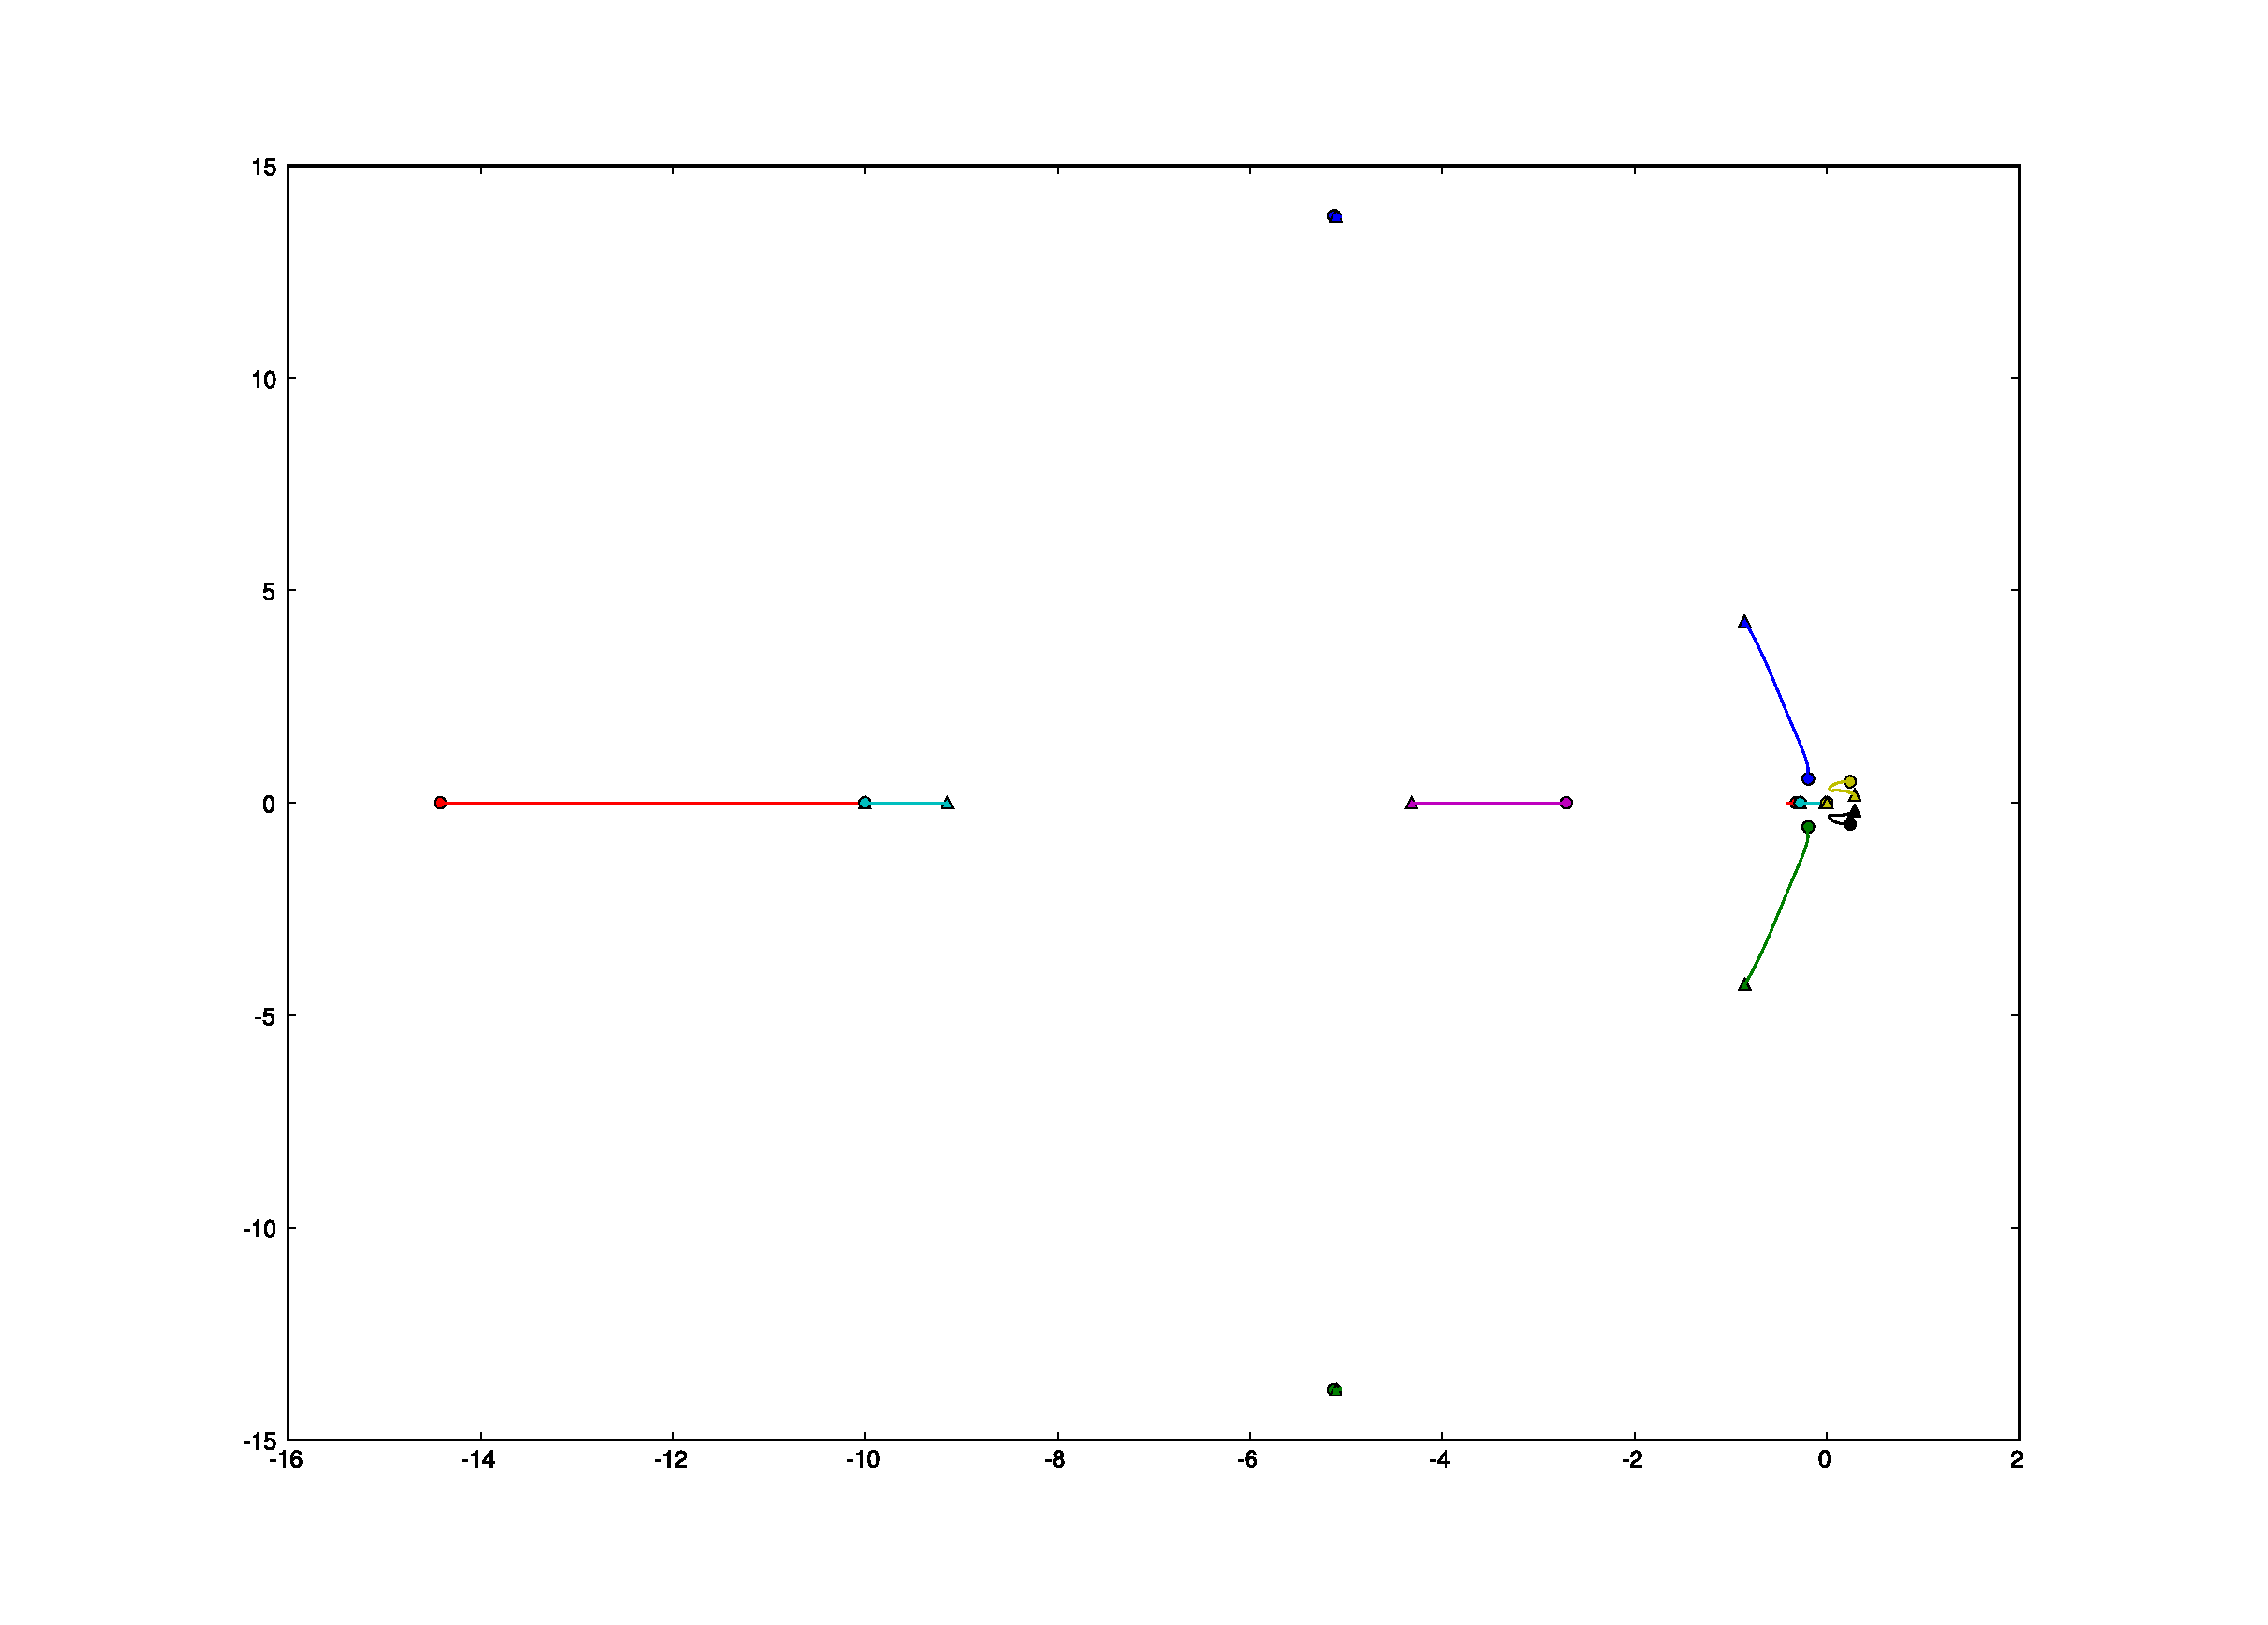
\includegraphics[scale=0.35]{Figuras/Lynx_modos.eps}
    \caption{Modos propios del Lynx}
    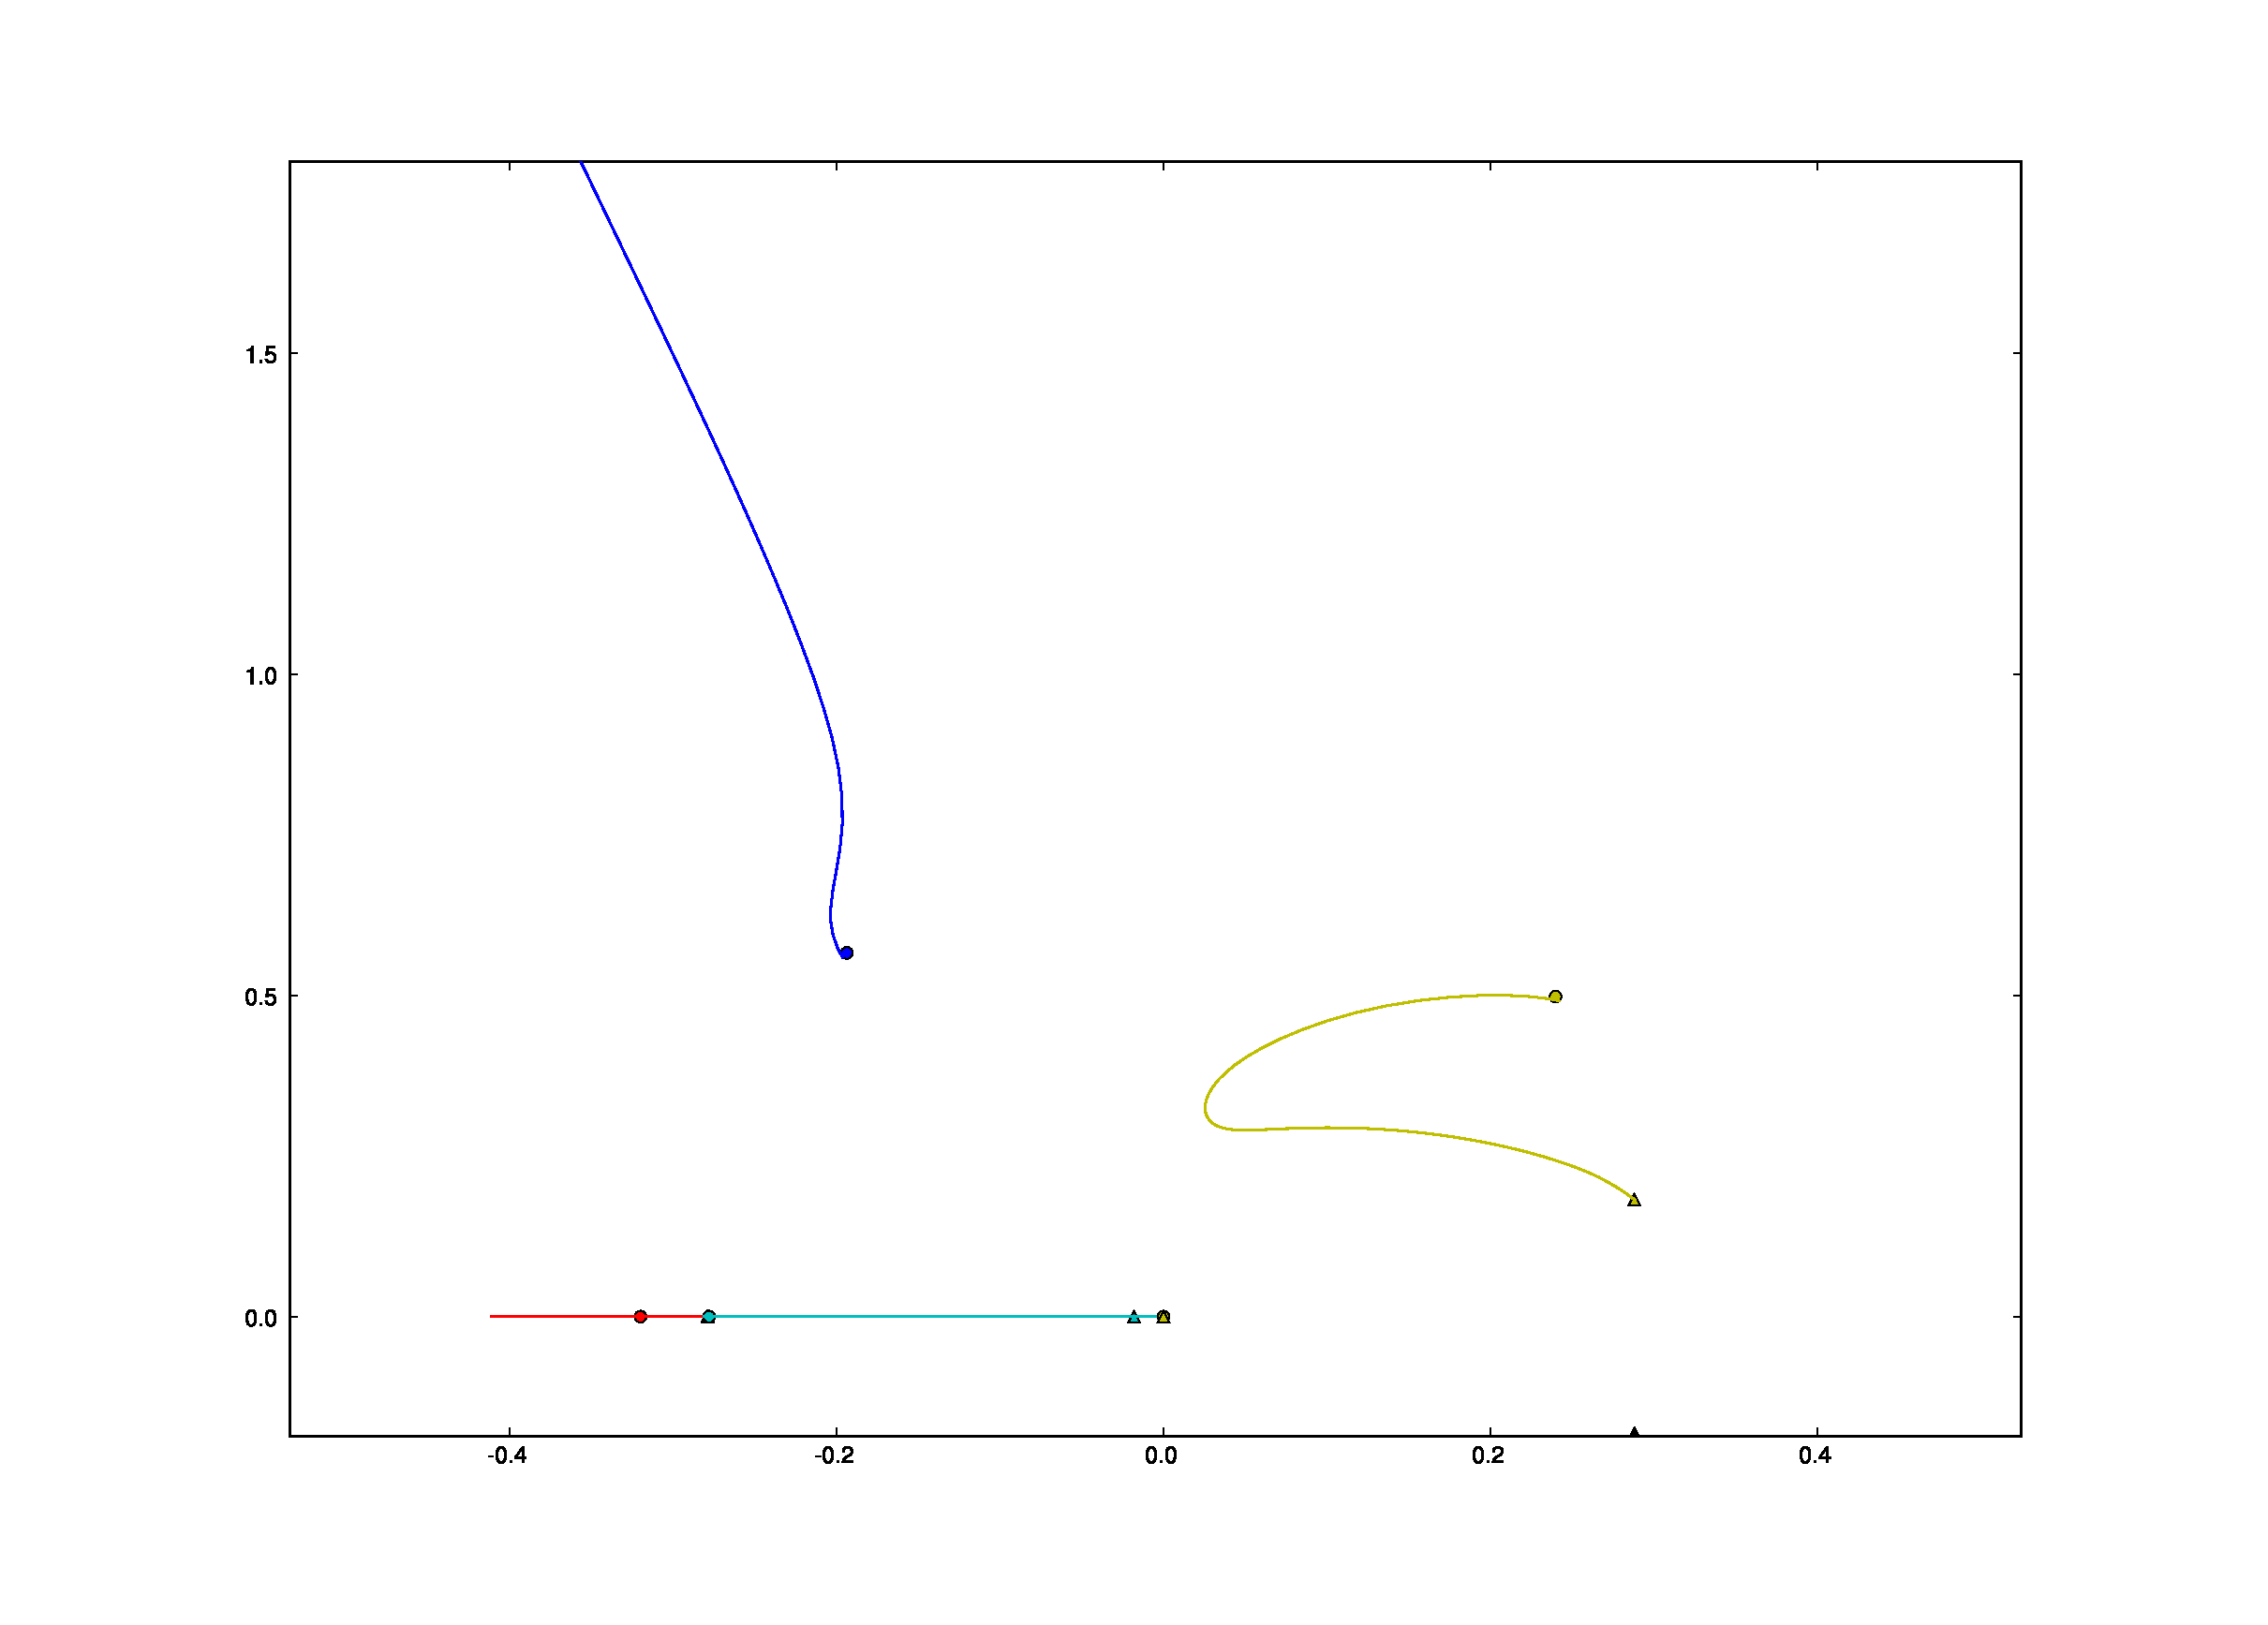
\includegraphics[scale=0.30]{Figuras/Lynx_modos_detalle.eps}
    \caption{Detalle cerca del origen}
    \label{fig:modos}
\end{figure}

Como se ve los modos m�s exigentes son el de convergencia en balance y sobre
todo el asociado al giro del motor, que presenta una componente imaginaria muy
alta. Teniendo en cuenta esto y que el paso de tiempo es del orden de 0.03
podemos descartar aquellos esquemas cuyas zonas de estabilidad no cubran los
anteriores modos escalados por el paso de tiempo.

A continuaci�n se discuten en qu� medida son
satisfactorios los integradores que se encuentran ya implementados. 

Para analizar la estabilidad del integrador se ha calculado la regi�n de
estabilidad de cada integrador resolviendo num�ricamente el polinomio 
(ver \cite{numerico}):

\begin{equation*}
    \sum_{j=0}^p \left(\alpha_j - \omega f_j(\omega)\right)r^{p-j} = 0
\end{equation*}

para diversos valores del n�mero complejo $\omega$. Se ha extra�do en cada punto
el valor de la ra�z de mayor valor absoluto $r_{max}$ y se han dibujado las l�neas de
nivel de contorno para $r_{max}\leq1$. Los valores de los anteriores coeficientes
vienen especificados en la discusi�n de cada integrador.

Para estimar la precisi�n de la soluci�n se ha calculado la respuesta del 
helic�ptero en un caso cualquiera con diferentes pasos de tiempo. Para ello se ha 
realizado un vuelo, se ha guardado en fichero las magnitudes en los diferentes instantes
de tiempo, incluidos los controles, se ha ``serializado'' el fichero de logging mediante
la utilidad \verb!serializa! y mediante un peque�o programa \verb!test_integrador! se ha
calculado la respuesta del helic�ptero en funci�n del tiempo para pasos de 0.03 y 0.015 
segundos. Se ha calculado el m�ximo error global que se presenta en el intervalo de tiempo
calculado y se han trazado las gr�ficas comparando ambas respuestas. La l�nea continua 
corresponde al paso menor y por tanto en teor�a m�s preciso de 0.015 segundos mientras
que los puntos, dibujados s�lo cada 0.3 segundos, corresponden al paso de 0.03 segundos. 
Como las gr�ficas a simple vista son indistinguibles unas de otras se muestra s�lo una, la
calculada para el Predictor-Corrector (figura \ref{fig:serie converge}) y otra, que no converge, 
para el Adams-Bashforth 3 (figura \ref{fig:serie no converge}).
En esta �ltima se ve c�mo se necesita un paso peque�o para que la zona de estabilidad abarque 
todos los autovalores de la ecuaci�n diferencial. 

\begin{figure}
    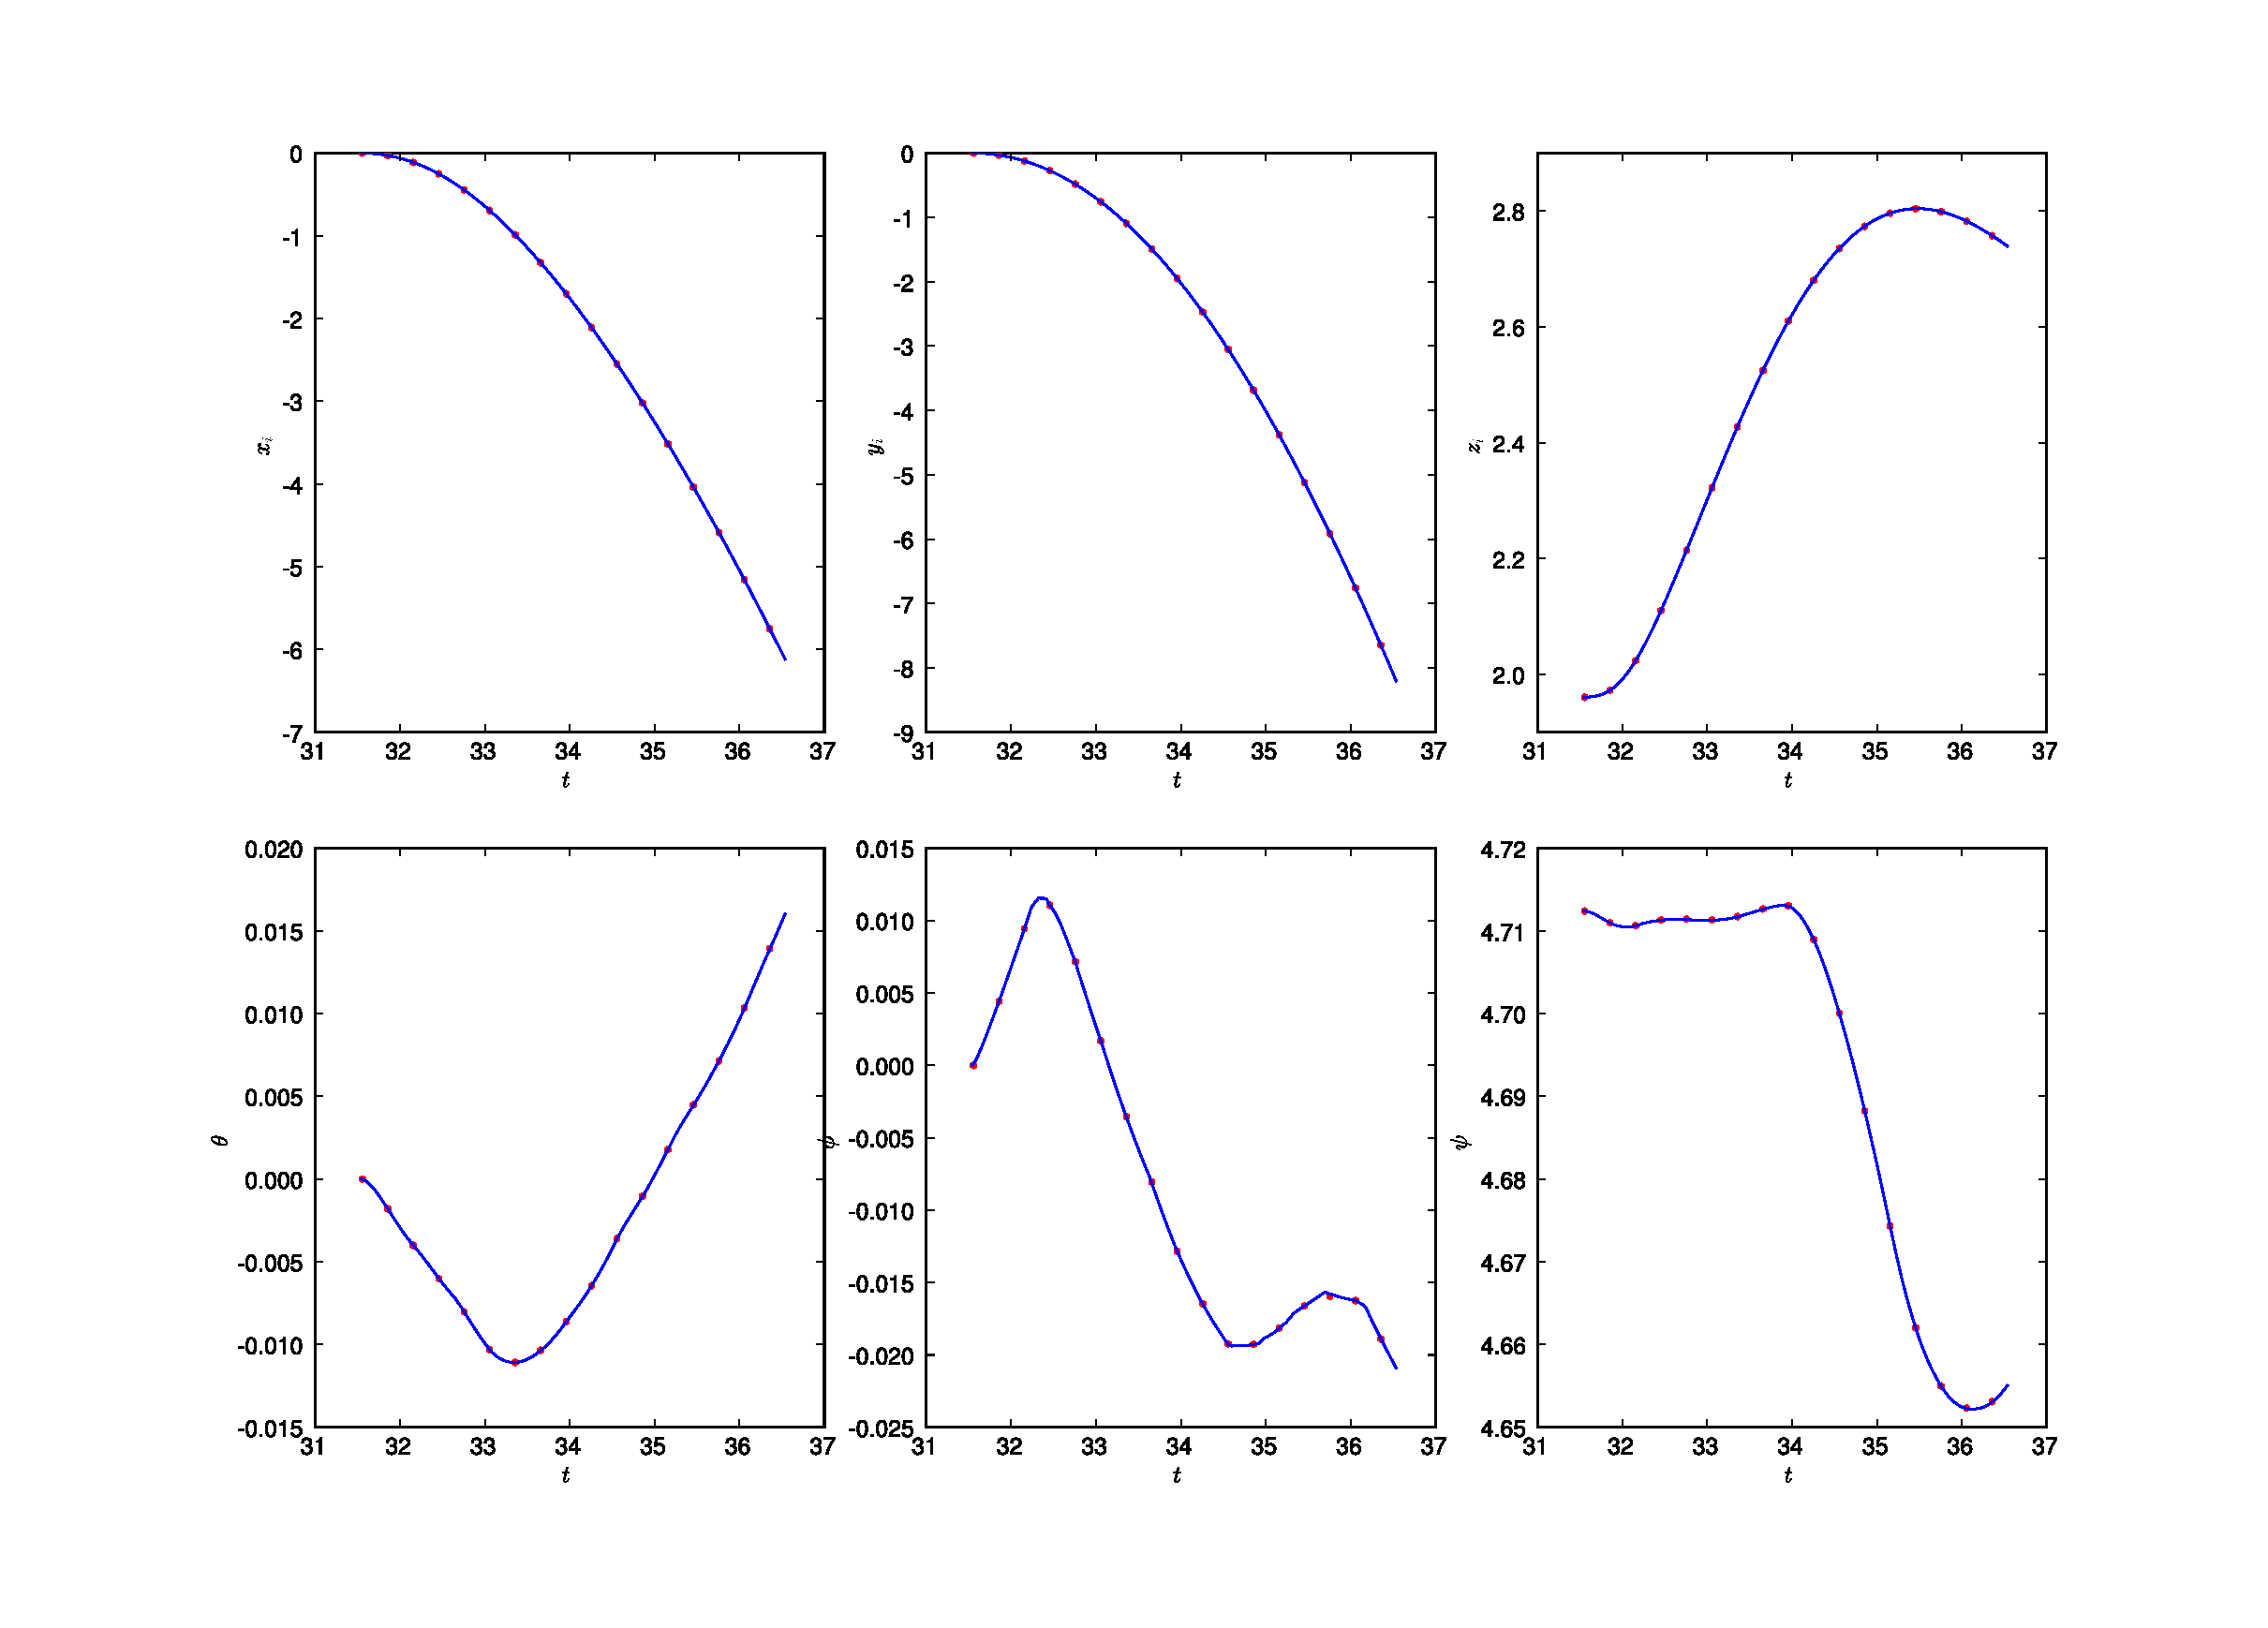
\includegraphics[scale=0.45,angle=90]{Figuras/integradores_series.eps}
    \caption{C�lculo de la posici�n y actitud del helic�ptero en funci�n del tiempo para
    dos pasos diferentes de integraci�n}
    \label{fig:serie converge}
\end{figure}


\subsection{Euler}
Es el primer integrador que se implement� debido a su sencillez. Su uso no se
recomienda ya que presenta p�simas caracter�sticas de estabilidad y un error
bastante pobre. A su favor hay que decir que por ser el m�s simple tambi�n es el
que menos tiempo requiere. En ocasiones ha llegado a fallar su estabilidad sobre
todo debido al grado de libertad asociado al giro del motor. Se mantiene en el
fichero de integradores para poder usarlo como plantilla para implementar otros
integradores.

\begin{equation*}
    u^{n+1} = u^n + \triangle tF^n
\end{equation*}

Polinomio de estabilidad:
\begin{align*}
    \alpha_0 &= 1 & f_0 &= 0 \\
    \alpha_1 &= -1 & f_1 &= 1 
\end{align*}

\begin{figure}
    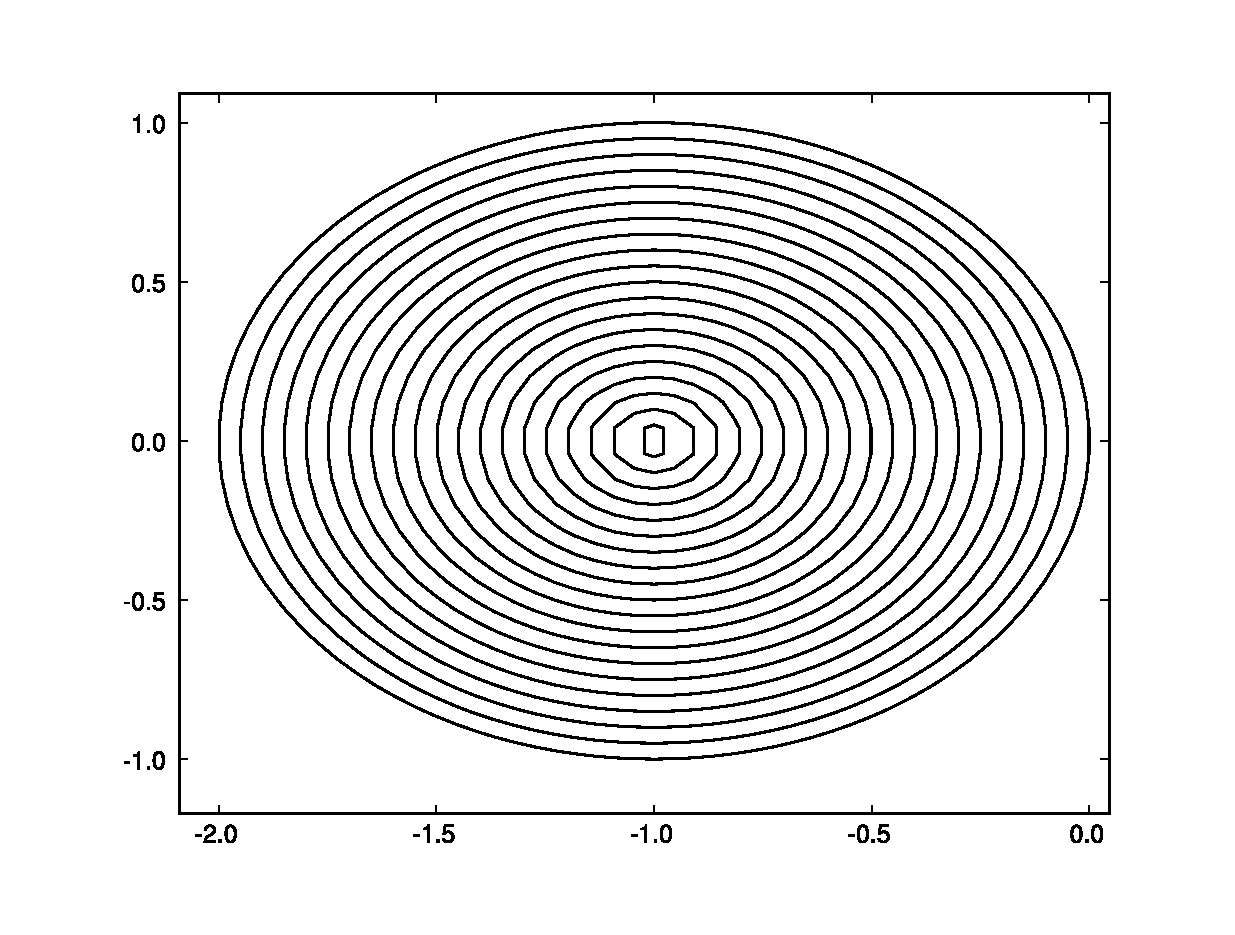
\includegraphics[scale=0.6]{Figuras/estabilidad_Euler.eps}
    \caption{Regi�n de estabilidad del Euler}
\end{figure}

El m�ximo error global para el peque�o vuelo de test ha correspondido a $y_i$, 
y ha sido de 0.031 metros.
    

\subsection{Runge-Kutta de orden 4}
Fue el segundo integrador que se implement� debido a sus excelentes propiedades
de estabilidad. Es el integrador a utilizar si se presenta alg�n problema de
divergencia explosiva en las ecuaciones ya que puede ayudar a identificar si se
trata de un error en el modelo o en el integrador. Desgraciadamente exige la
evaluaci�n de la funci�n en cuatro puntos intermedios por lo que es el peor
integrador a usar para ahorrar coste computacional. No se recomienda su uso si
se va a utilizar el simulador interactivamente ya que debido a que se encuentra
implementado en python, un lenguaje interpretado bastante lento (30 veces m�s
lento que C), se producir�an desfases intolerables entre las acciones del piloto
y la respuesta del helic�ptero. Esto es un fallo de implementaci�n del
simulador, en futuras mejoras habr�a que reimplementar las partes que m�s tiempo
consumen en C/C++ u otro lenguaje de bajo nivel.

\begin{align*}
    u^{n+1} &= u^n + \frac{\triangle t}{6}(k_1 + 2k_2 + 2k_3 + k_4) \\
    k_1 &= F(u^n, t_n) \\
    k_1 &= F(u^n + \triangle t k_1/2, t_n + \triangle t/2) \\
    k_1 &= F(u^n + \triangle t k_2/2, t_n + \triangle t/2) \\
    k_1 &= F(u^n + \triangle tk_3, t_n + \triangle t) \\
\end{align*}

Polinomio de estabilidad:
\begin{align*}
    \alpha_0 &= 1 & f_0 &= 0 \\
    \alpha_1 &= -1 & f_1 &= \frac{1}{24}(w^3 + 4w^2 + 12w + 24) \\
\end{align*}

\begin{figure}
    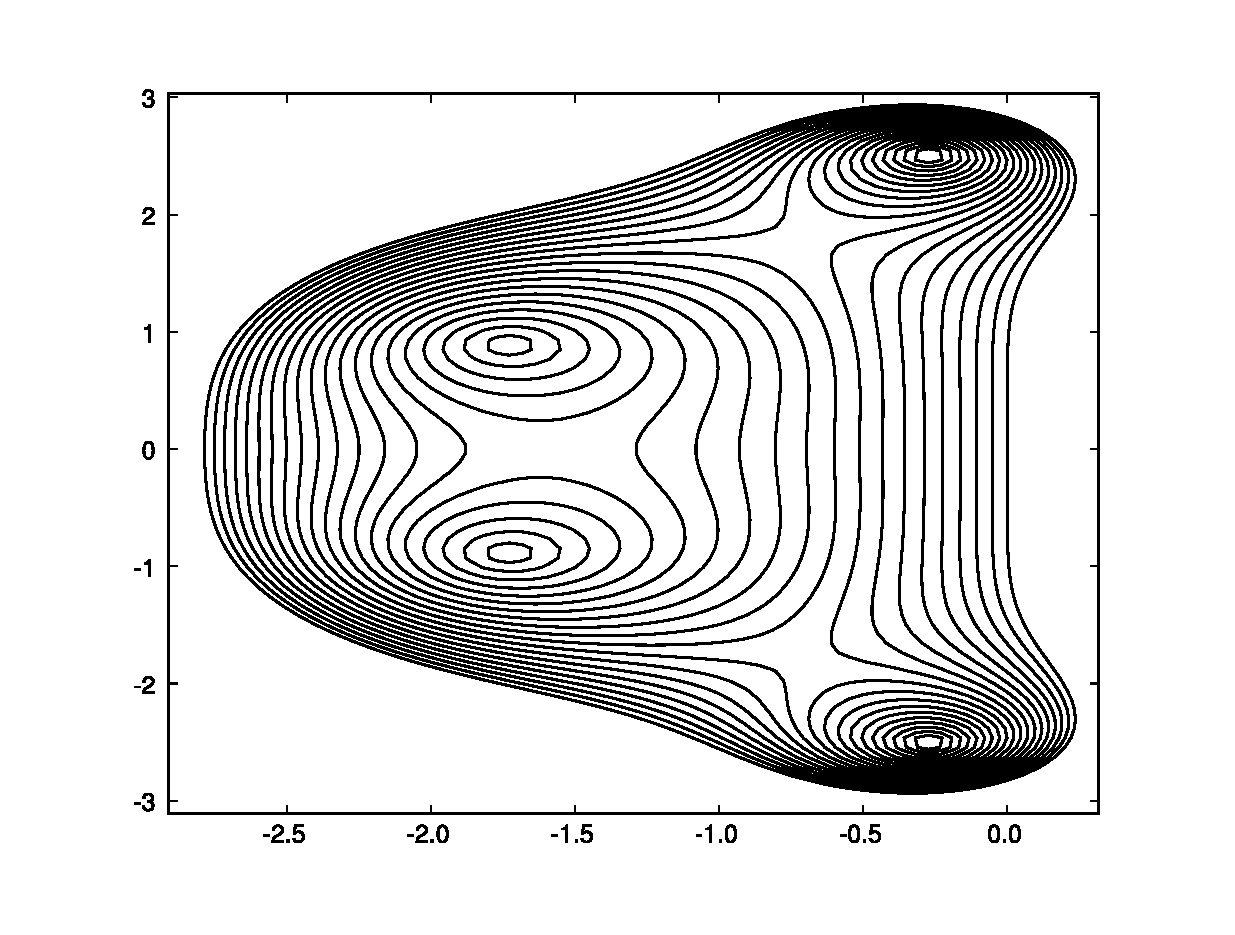
\includegraphics[scale=0.6]{Figuras/estabilidad_RK4.eps}
    \caption{Regi�n de estabilidad del Runge-Kutta 4}
\end{figure}

El m�ximo error global para el peque�o vuelo de test ha correspondido a $y_i$, 
y ha sido de 0.049 metros.

\subsection{Adams-Bashforth 2}
Mejora las caracter�sticas del Euler y adem�s no exige evaluaciones
adicionales de la funci�n. Es uno de los dos integradores recomendados para todo
uso.

\begin{align*}
    u^{n+1} &= u^n + \triangle t(\beta_1 F^n + \beta_2F^{n-1}) \\
    \beta_1 &= \frac{2\triangle t_2 + \triangle t_1}{2\triangle t_2} \\
    \beta_2 &= -\frac{\triangle t_1}{2\triangle t_2}
\end{align*}

Polinomio de estabilidad (para paso constante):
\begin{align*}
    \alpha_0 &= 1 & f_0 &= 0 \\
    \alpha_1 &= -1 & f_1 &= \frac{3}{2} \\
    & & f_2 &= -\frac{1}{2}
\end{align*}

\begin{figure}
    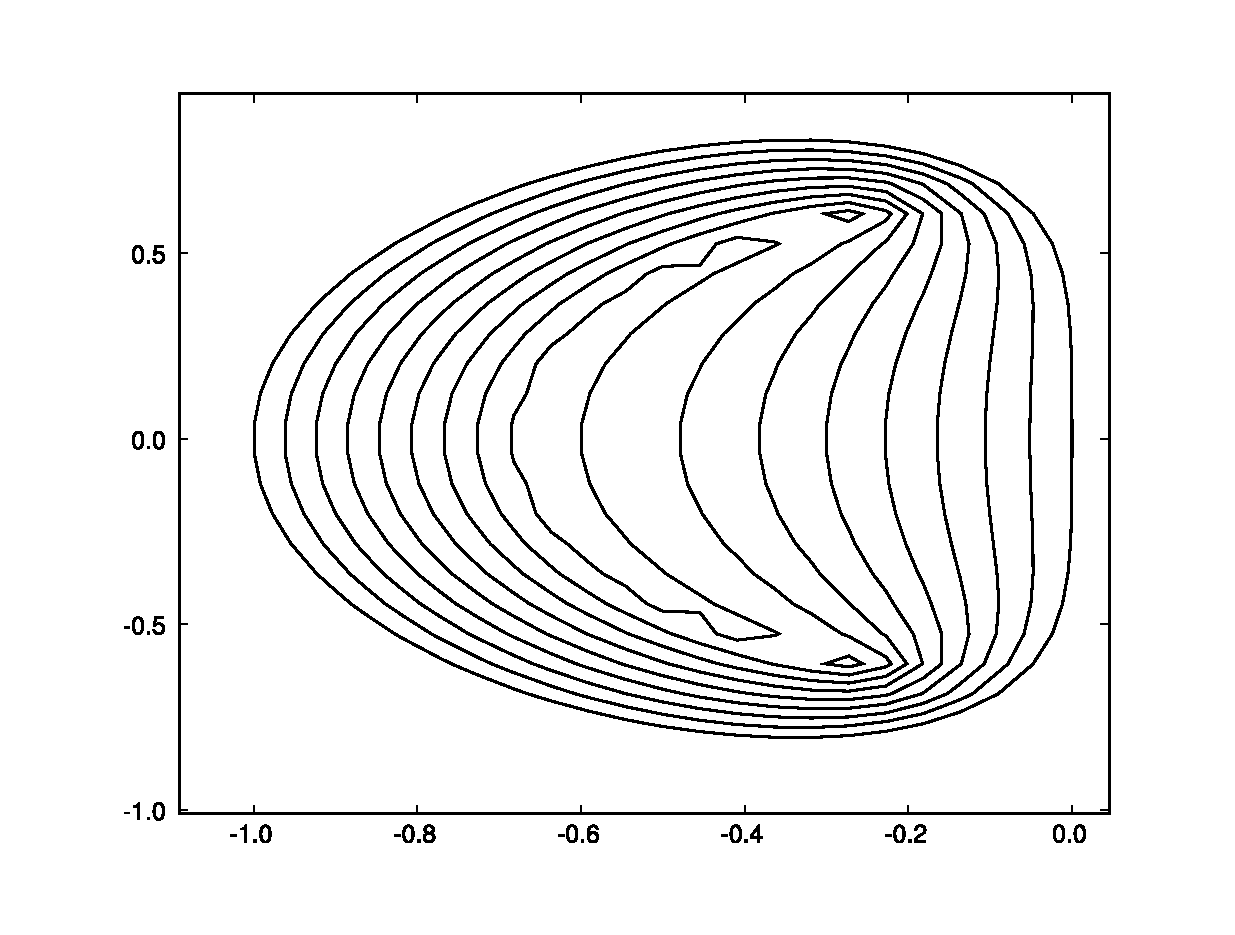
\includegraphics[scale=0.6]{Figuras/estabilidad_AB2.eps}
    \caption{Regi�n de estabilidad del Adams-Bashforth 2}
\end{figure}

El m�ximo error global para el peque�o vuelo de test ha correspondido a $x_i$, 
y ha sido de 0.001 metros.

\subsection{Adams-Bashforth 3}
Se ha implementado este integrador para ver si se pod�a mejorar la precisi�n del
Adams-Bashfort 2. Desgraciadamente no es un integrador adecuado, ya que requiere
pasos de tiempo la mitad de peque�os que el Adams-Bashofrth 2, por lo que puede
llegar a diverger.

\begin{align*}
    u^{n+1} &= u^n + \triangle t(\beta_1 F^n + \beta_2F^{n-1} + \beta_3F^{n-2}) \\
    \beta_1 &= 1 + \frac{\triangle t_1\left(2\triangle t_1 + 6\triangle t_2 +
    3\triangle t_3\right)}{6\triangle t_2\left(\triangle t_2 + \triangle
    t_3\right)} \\
    \beta_2 &= -\frac{\triangle t_1\left(2\triangle t_1 + 3\triangle t_2 +
    3\triangle t_3\right)}{6\triangle t_2 \triangle t_3} \\
    \beta_3 &= \frac{\triangle t_1\left(2\triangle t_1 + 3\triangle t_2
    \right)}{6\triangle t_3\left(\triangle t_2 + \triangle t_3\right)}
\end{align*}

Polinomio de estabilidad (para paso constante):
\begin{align*}
    \alpha_0 &= 1 & f_0 &= 0 \\
    \alpha_1 &= -1 & f_1 &= \frac{23}{12} \\
    & & f_2 &= -\frac{4}{3} \\
    & & f_3 &= \frac{5}{12}
\end{align*}

\begin{figure}
    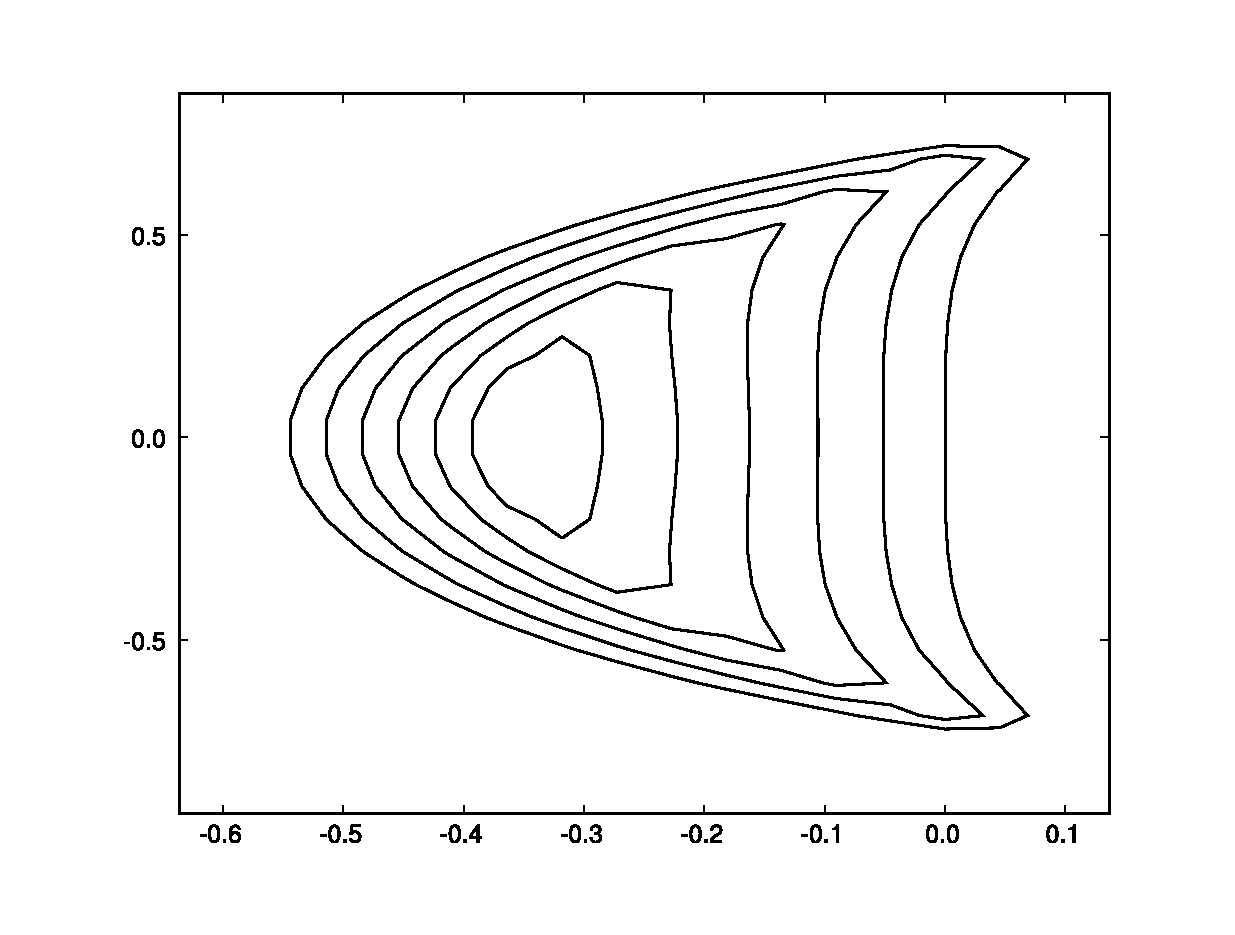
\includegraphics[scale=0.6]{Figuras/estabilidad_AB3.eps}
    \caption{Regi�n de estabilidad del Adams-Bashforth 3}
\end{figure}

Para paso de 0.03 segundos el m�todo se ha vuelto inestable.
\begin{figure}
    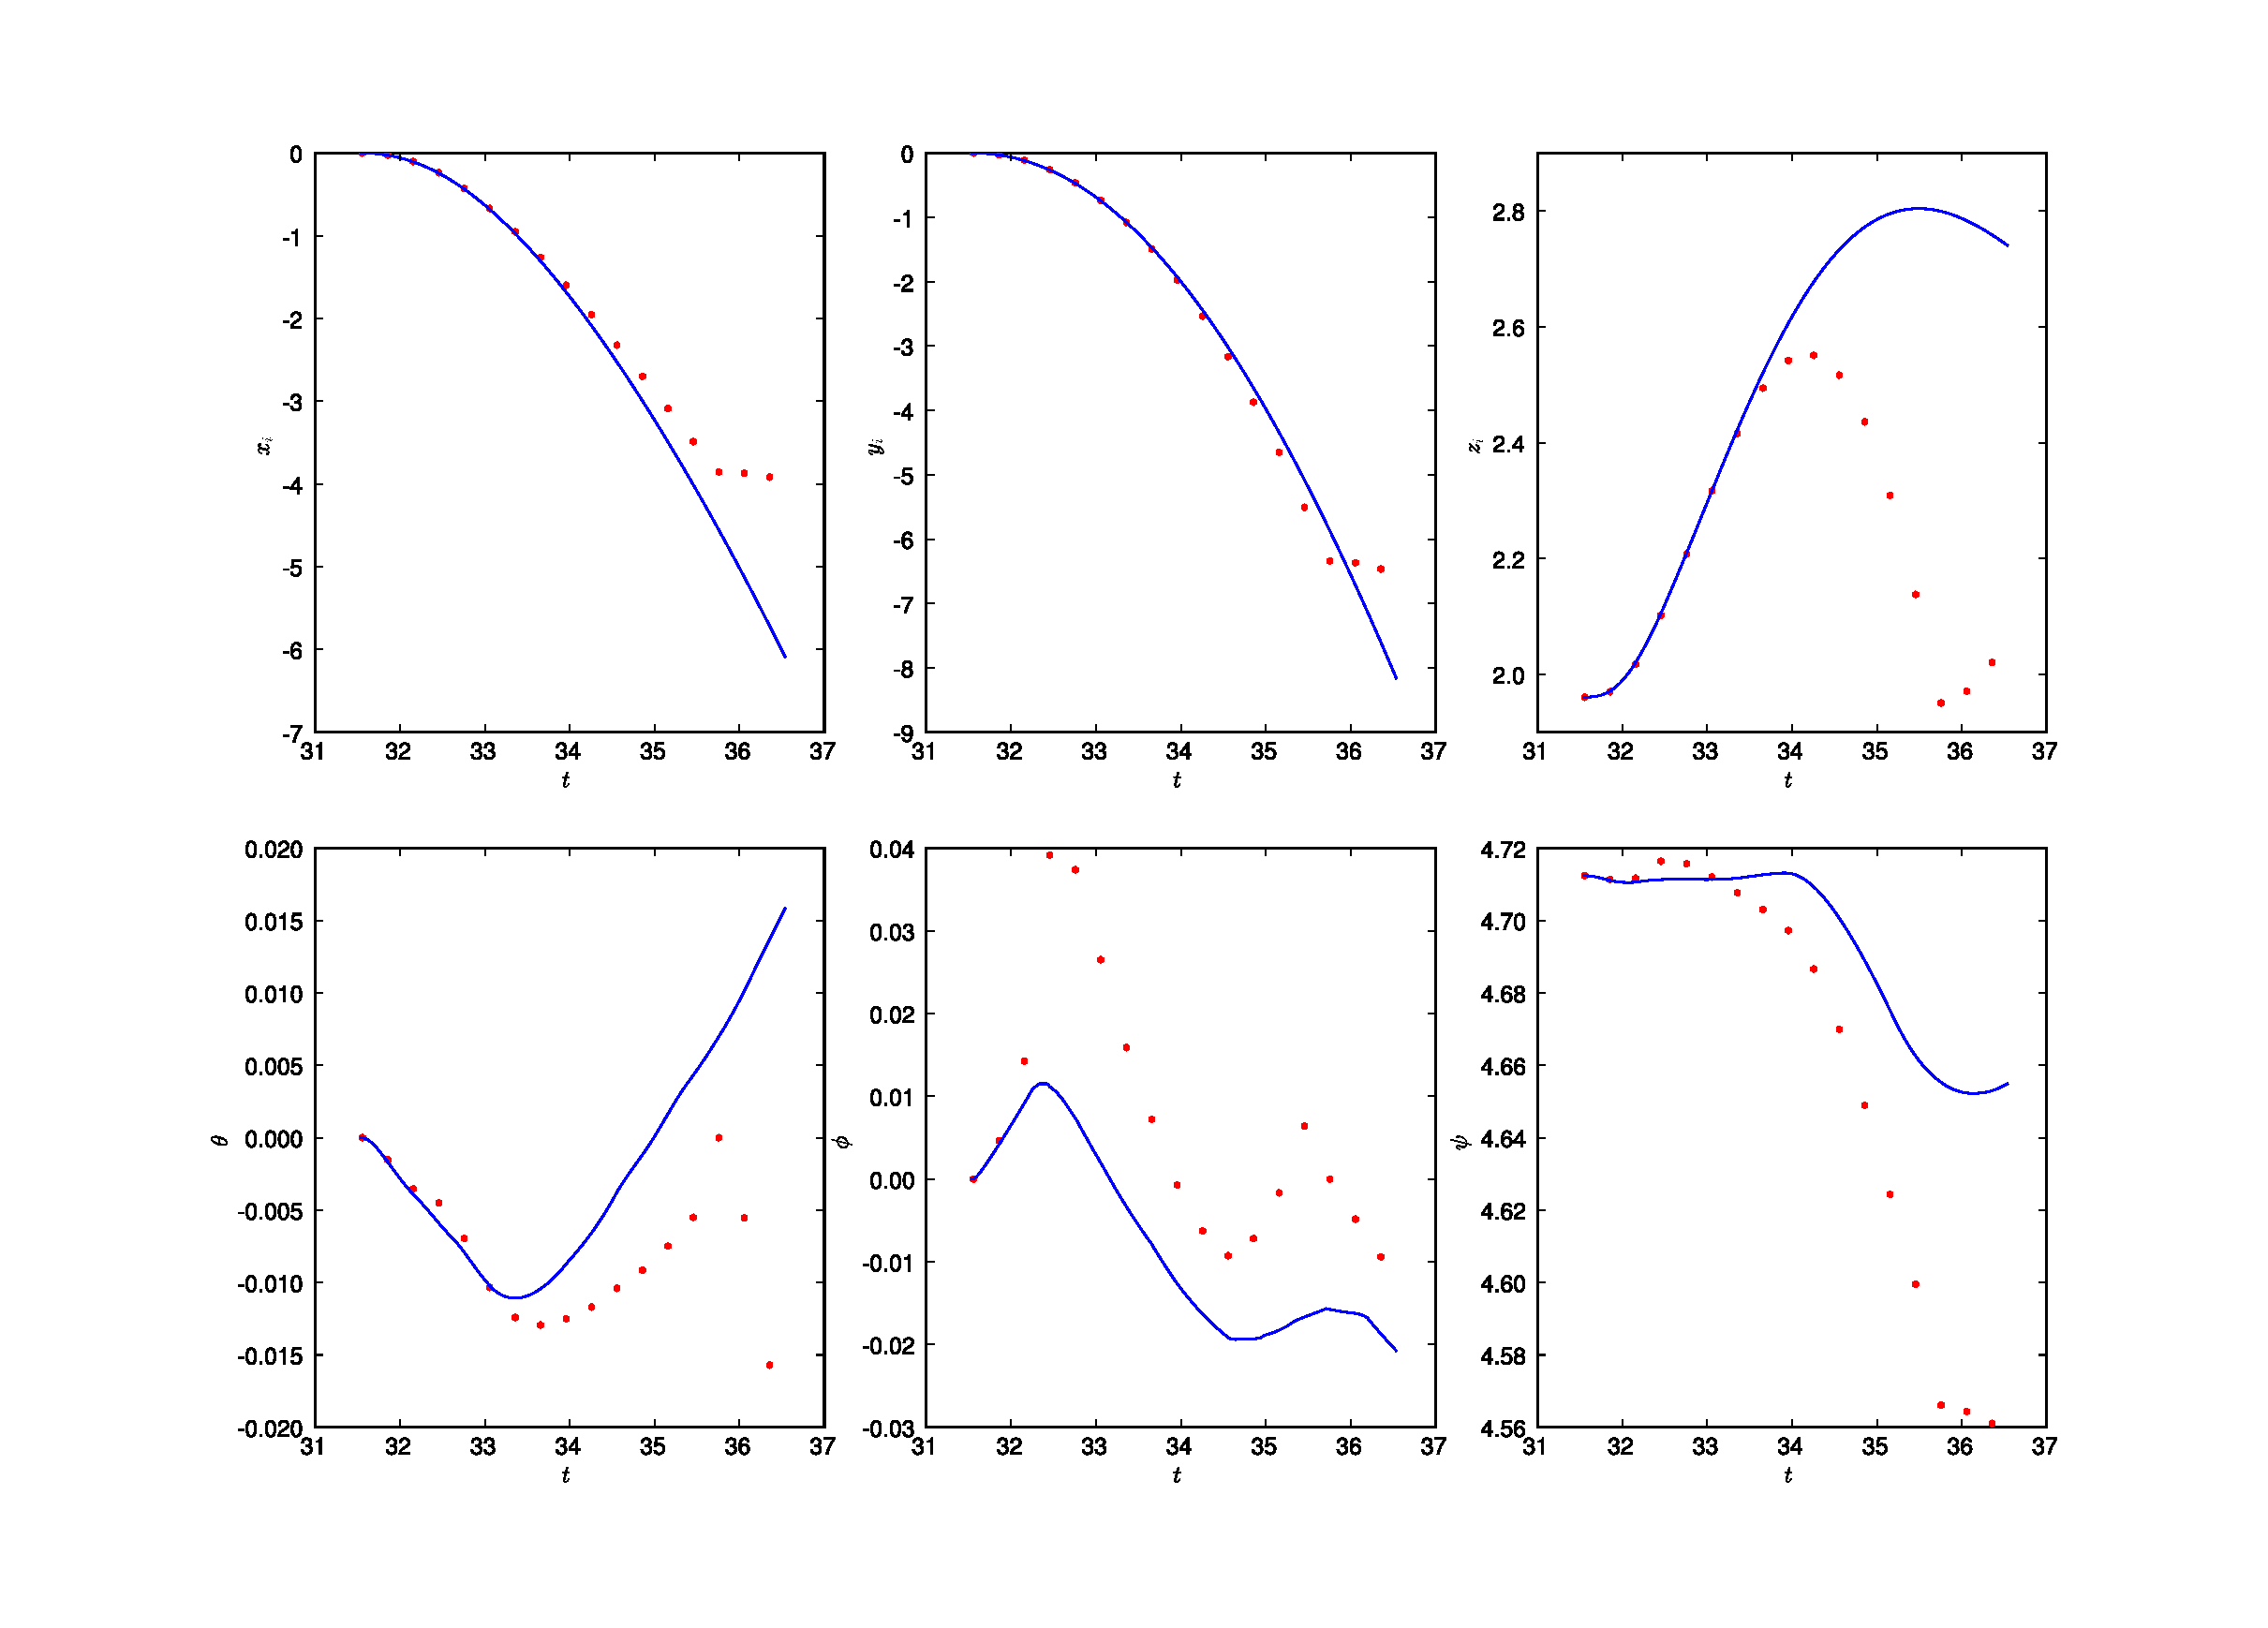
\includegraphics[scale=0.45,angle=90]{Figuras/integradores_series_mal.eps}
    \caption{Inestabilidad del Adams-Bashforth 3}
    \label{fig:serie no converge}
\end{figure}

\subsection{Predictor-Corrector Adams-Bashforth-Moulton 2}
Finalmente el mejor integrador para esta aplicaci�n presenta una zona de
estabilidad suficientemente grande y s�lo requiere dos evaluaciones de la
funci�n en cada instante de tiempo por lo que es suficientemente r�pido para
ejecutarlo en modo interactivo. Como valor a�adido permite estimar el error
num�rico.


\begin{align*}
    u_*^{n+1} &= u^n + \triangle t(\beta_{p1} F^n + \beta_{p2}F^{n-1}) \\
    F_*^{n+1} &= F(u_*^{n+1}, t_{n+1}) \\
    u^{n+1} &= u^n + \triangle t(\beta_{c0}F_*^{n+1} + \beta_{c1}F^n) \\
    \beta_{p_1} &= \frac{2\triangle t_2 + \triangle t_1}{2\triangle t_2}  &
    \beta_{c_0} &= \frac{1}{2}\\
    \beta_{p_2} &= -\frac{\triangle t_1}{2\triangle t_2} & 
    \beta_{c_1} &= \frac{1}{2}\\
\end{align*}

Polinomio de estabilidad (para paso constante):
\begin{align*}
    \alpha_0 &= 1 & f_0 &= 0 \\
    \alpha_1 &= -1 & f_1 &= 1 + \frac{3}{4}\omega \\
    & & f_2 &= -\frac{1}{4}\omega
\end{align*}

\begin{figure}
    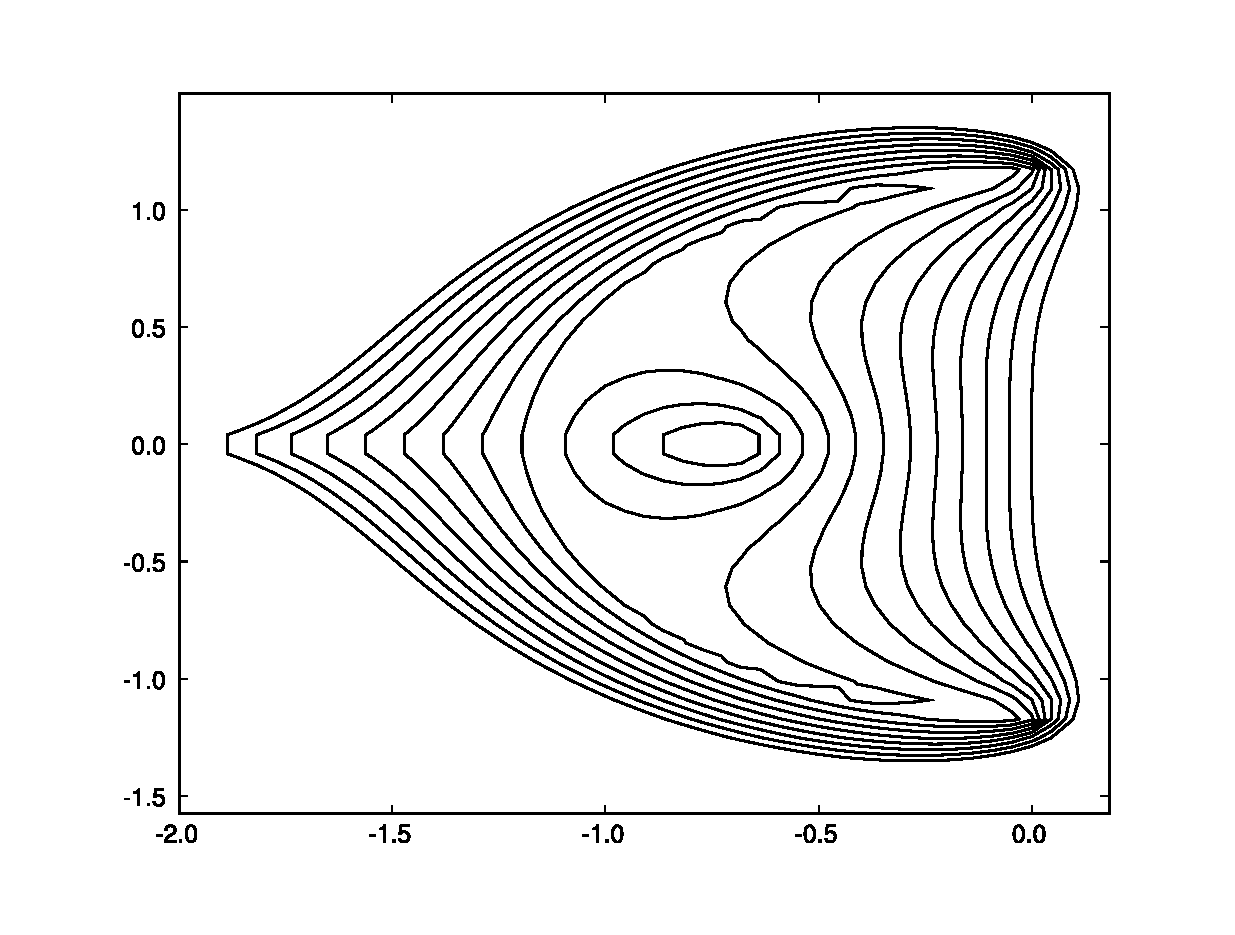
\includegraphics[scale=0.6]{Figuras/estabilidad_ABM2.eps}
    \caption{Regi�n de estabilidad del Adams-Bashforth-Moulton 2}
\end{figure}

El m�ximo error global para el peque�o vuelo de test ha correspondido a $y_i$, 
y ha sido de 0.061 metros.

\chapter{Trimado}
Para calcular la posici�n de equilibrio del helic�ptero es necesario resolver
por lo menos un conjunto de 15 ecuaciones:
\begin{itemize}
  \item 6 Ecuaciones de fuerzas y momentos del fuselaje.
  \item 3 Ecuaciones de orientaci�n del helic�ptero.
  \item 1 ecuaci�n para la velocidad de rotaci�n del rotor.
  \item 1 ecuaci�n para el c�lculo de par de motor a partir de la velocidad
	  del rotor.
  \item 4 ecuaciones adicionales, tantas como controles tiene el helic�ptero
	  para igualar el n�mero de inc�gnitas con el de ecuaciones.
\end{itemize}

Muchas de las anteriores ecuaciones son no lineales:
\begin{itemize}
	\item  Las fuerzas de inercia dependen cuadr�ticamente de la velocidad y
		la velocidad angular.
	\item  La fuerza de la gravedad depende mediante funciones
		trigonom�tricas del cabeceo y del balance.
	\item  Tambi�n dependen de la misma forma las fuerzas aerodin�micas que
		adem�s se pueden encontrar dadas en forma de tablas para
		interpolar.
	\item  Las fuerzas del rotor dependen linealmente y cuadr�ticamente del
		batimiento y trigonom�tricamente de la orientaci�n.
	\item La velocidad inducida en el rotor depende de forma no lineal del
		coeficiente de sustentaci�n.
	\item El resto de ecuaciones son lineales: los controles en funci�n de
		los pasos y las ecuaciones del batimiento y la velocidad
		inducida no uniforme.
\end{itemize}

Adem�s, debido a las caracter�sticas del helic�ptero, se trata de un sistema
totalmente acoplado y que por ejemplo, el control longitudinal del paso del
rotor influye sobre el batimiento lateral, lo que provoca momentos y fuerzas
laterales, etc\ldots

A falta de un mejor an�lisis matem�tico del problema la estrategia que se ha seguido para resolver el
trimado ha sido siguiendo un razonamiento f�sico, similar al que seguir�a un
piloto a los mandos del helic�ptero: primero y a pesar de todo, dividir el problema en
una parte longitudinal y otra lateral. Se resuelven secuencialmente las
ecuaciones longitudinales y se iteran hasta que converge un determinado
par�metro, por ejemplo el cabeceo del helic�ptero. Se hace de la misma forma
para las ecuaciones laterales utilizando como par�metro el �ngulo de balance.
Finalmente se itera en la velocidad angular y se resuelven las ecuaciones

\section{Condiciones adicionales}

Especificamos las condiciones de trimado dadas, por ejemplo, por
los siguientes 4 par�metros, aunque podr�an haber sido otros:
\begin{itemize}
  \item Velocidad de giro $\Omega_a$.
  \item Velocidad $V$.
  \item �ngulo de subida $\gamma_f$.
  \item �ngulo de resbalamiento $\beta$.
\end{itemize}

\section[Velocidad y vel. angular]{C�lculo de la velocidad y velocidad angular}

Conocidos estos cuatro par�metros, suponemos conocidos, ya sea de una estimaci�n
inicial o de un c�lculo anterior el valor de cabeceo $\theta$ y el de balance
$\phi$, entonces podemos calcular la velocidad  $u,v,w$ y la velocidad angular
$p, q, r$ en ejes cuerpo. La velocidad angular se calcula r�pidamente utilizando
las relaciones usuales para �ngulos de Euler:

\begin{align*}
	p &= -\Omega_a\sin\theta \\
	q &= \Omega_a\cos\theta\sin\phi \\
	r &= \Omega_a\cos\theta\cos\phi
\end{align*}

El c�lculo de la velocidad es un poco m�s elaborado. Para ello expresamos la
velocidad en ejes cuerpo y en unos ejes inerciales:
\begin{align*}
	\vec{V} &= V\left[\frac{u}{V}\vec{i}_b + \sin\beta\vec{j}_b +
	\frac{w}{V}\vec{k}_b\right] \\
	&= V\left[\cos\gamma\cos\chi\vec{i}_0 + \cos\gamma\sin\chi\vec{j}_0 +
	\sin\gamma\vec{k}_0\right] \\
\end{align*}

Donde el �ngulo $\chi$ es el �ngulo que forma la proyecci�n de la velocidad
sobre el $x_0y_0$ con el eje $x_0$, y constituye una inc�gnita junto con $u$ y
$v$.

Utilizando la matriz de cambio de base de ejes inerciales a ejes cuerpo que se
obtuvo en el cap�tulo dedicado a sistemas de referencia obtenemos 3 ecuaciones.
Resolviendo una de ellas:

\begin{equation*}
    \sin\beta - \sin\gamma\sin\phi\cos\theta =
    \cos\gamma\sin\theta\sin\phi\cos(\chi - \psi) + \cos\gamma\cos\phi\sin(\chi
    - \phi) 
\end{equation*}

De donde despejamos el �ngulo $\chi - \psi$. Una vez conocido este �ngulo
obtenemos de las otras dos ecuaciones:
\begin{align*}
	\frac{u}{V} &= \cos\theta\cos\gamma\cos(\chi - \psi) -
	\sin\theta\sin\gamma \\
	\frac{w}{V} &= \cos\gamma\sin\theta\cos\phi\cos(\chi-\psi) +
	\cos\gamma\sin\phi\sin(\chi-\psi) +\\
	&\sin\gamma\cos\phi\cos\theta 
\end{align*}

La anterior ecuaci�n para $\chi - \psi$ tiene dos soluciones que se 
corresponden a distintos �ngulos de ataque para el helic�ptero. Para entender
esta multiplicidad de soluciones podemos visualizar la condici�n en $\gamma$
como un requisito para que la velocidad se encuentre en el cono de semi�ngulo
$\frac{\pi}{2} - \gamma$ que tiene como eje el eje $z_0$, y la condici�n en
$\beta$ como otro requisito para que la velocidad se encuentre en un cono de
semi�ngulo $\frac{\pi}{2} - \beta$ con eje el $y_B$. La velocidad ser� entonces
la intersecci�n de los dos anteriores conos que comparten su v�rtice, por lo que
habr� dos soluciones en general aunque puede que no haya ninguna o incluso una,
si ambos conos son tangentes.

\begin{figure}
	\input{Figuras/conoGamma.pstex_t}
	\caption{Posibles soluciones de $\vec{V}$}
\end{figure}

De las dos soluciones nos quedamos con la que f�sicamente tiene mas sentido, que es
la que de el menor valor de �ngulo de ataque. En el caso de no haber soluci�n
habr�a que reintroducir alguno de los cuatro par�metros.

\section[Fzas. aerodin�micas y de inercia]
{C�lculo de fuerzas aerodin�micas y de inercia}
Conocida  la velocidad en ejes cuerpo y supuestos c�lculos anteriores para la
velocidad inducida y �ngulo de estela podemos determinar las fuerzas
aerodin�micas de fuselaje y estabilizadores, y tambi�n determinamos las fuerzas
de inercia. Calculamos tambi�n los ejes viento del rotor y cola, par�metros de
avance y velocidades angulares adimensionalizadas con la velocidad de giro del
rotor (suponemos conocida tambi�n).

\section{Ecuaciones longitudinales}
Suponemos conocidas las fuerzas y momentos del rotor de cola. A continuaci�n
vamos a hacer cumplir las ecuaciones longitudinales del movimiento, para ello
vamos a suponer que nuestros par�metros de control son la tracci�n del rotor
$c_T$ para hacer cumplir la ecuaci�n de fuerzas vertical, el batimiento 
longitudinal $\beta_{1c}$ para hacer cumplir la ecuaci�n de momentos de cabeceo y el
�ngulo de cabeceo $\theta$ que inclina la tracci�n del rotor para vencer la
resistencia aerodin�mica sobre todo del fuselaje. M�s detalladamente:

\begin{enumerate}
	\item Despejamos la fuerza vertical del rotor en ejes cuerpo $Z_R$,
		normalmente un valor cercano al peso del helic�ptero que se
		puede utilizar como primera aproximaci�n.
        \begin{equation*}
		    Z_R = M(-qu + pv) - (Z_f + Z_{fn} + Z_{tp} + Z_{T}) -
		    Mg\cos\theta 
        \end{equation*}
	
	\item Despejamos el momento del rotor en ejes cuerpo de la ecuaci�n de
		momentos de cabeceo:
        \begin{equation*}
		    M_R = -(I_{zz} - I_{xx})rp - I_{xz}(r^2 - p^2) - (M_f + M_{fn}
		    + M_{tp} + M_T) 
        \end{equation*}
	
	\item Suponiendo conocida la fuerza horizontal del rotor calculamos las
		fuerzas y momentos aplicados sobre la cabeza del
		rotor:
		\begin{align*}
			X_{Rh} &= X_R \\
			Z_{Rh} &= Z_R \\
            M_{Rh} &= M_R - Z_R x_{cg} + X_R h_R \\
		\end{align*}
	
	\item Obtenemos el coeficiente de sustentaci�n del rotor a partir
        de las fuerzas y momentos en ejes viento:
        \begin{equation*}
		    c_T = -\frac{Z_{Rh_w}}{\rho(\Omega R)^2\pi R^2}
        \end{equation*}
	\item Obtenemos el batimiento del rotor
        \begin{equation*}
            \beta_{1cw} = \frac{-2M_{Rh_w}}{N_bK_\beta} 
        \end{equation*}
	
	\item Conocido $c_T$ y por tanto el coeficiente $\delta = \delta_0 +
		\delta_2 c_T^2$ y el batimiento $\beta_{1cw}$ ya podemos obtener
		una estimaci�n buena de la resistencia del rotor, calculamos
		$\left.X_{Rh}\right|_w$ donde suponemos conocidos los numerosos
		datos que faltan, que de todas formas influyen mucho menos:
		$\lambda_{1cw}$, $\lambda_{1sw}$, etc\ldots Pasamos a ejes
		cuerpo y tenemos $X_R$

	\item Despejamos de las ecuaciones horizontal y vertical la fuerza de 
		gravedad:
        \begin{equation*}
            \theta = \arctan\left(-\cos\phi\frac{M(-rv + qw) - (X_f +
		    X_{fn} + X_{tp} + X_T + X_R)}{M(-qu+pv) - (Z_f + Z_{fn} + Z_{tp}
		    + Z_T + Z_R)}\right) 
        \end{equation*}

	\item Comprobamos el error en $\theta$, es decir, su diferencia respecto
		al valor anteriormente calculado. Si no cae dentro del error
		admisible repetimos el proceso, si es aceptable pasamos al
		cumplimiento de las ecuaciones laterales
\end{enumerate}

\section{Ecuaciones laterales}
A continuaci�n hacemos cumplir las ecuaciones laterales, nuestras variables de
control van a ser la tracci�n de la cola $c_{T_T}$ para hacer cumplir la
ecuaci�n de momentos de gui�ada, el batimiento $\beta_{1s}$ para cumplir el
momento de balance y el �ngulo de balance $\phi$ para contrarrestar mediante el
rotor la fuerza lateral del rotor de cola.

\begin{enumerate}
	\item Una vez conocido $c_T$ del anterior bucle calculamos la velocidad
		inducida media $\lambda_0$ que nos permite junto a a $c_T$ 
		calcular el par del rotor, para ello resolvemos la ecuaci�n no
		lineal:
        \begin{equation*}
		    \frac{\lambda_0}{k_i} = \frac{c_T}{2\sqrt{\left(\frac{\mu}{k_\nu}
		    \right)^2 + \left(\frac{1}{k_\nu}^2 - \frac{1}{k_i}^2\right)\mu_z^2
		    + \left(\frac{\mu_z -\lambda_0}{k_i}\right)^2}} 
        \end{equation*}

		Donde ahora es $c_T$ una constante que no depende de $\lambda_0$.
	
	\item Calculamos el par del rotor en la cabeza del rotor en ejes viento
		y los pasamos al centro de masas en ejes cuerpo.

	\item De la ecuaci�n del momento de gui�ada despejamos el par que 
		realiza el rotor de cola.
        \begin{equation*}
            N_T = -(I_{xx} - I_{yy})pq + I_{xz}qr - (N_f + N_{fn} + N_{tp}
		        + N_R)
        \end{equation*}
		Despejamos del par del rotor de cola la sustentaci�n del rotor
		de cola:
        \begin{equation*}
		    Y_T = T_T = -\frac{N_T}{l_T + x_{cg}}
        \end{equation*}
	
	\item Con la tracci�n del rotor de cola podemos estimar bien el momento
		de balance provocado por el rotor de cola:
        \begin{equation*}
            L_T = Y_Th_T
        \end{equation*}
		Y despejar de la ecuaci�n del momento de balance el momento que
		debe de realizar el rotor:
        \begin{equation*}
            L_R = (I_{xx} - I_{yy})qr - I_{xz}pq - (L_f + L_{fn} + L_{tp}
		    + L_T)
        \end{equation*}
		Calculamos el momento de balance en la cabeza del rotor:
        \begin{equation*}
            L_{Rh} = L_R - Y_Rh_R
        \end{equation*}
		Y despejamos el batimiento lateral en ejes viento:
        \begin{equation*}
            \beta_{1sw} = -\frac{L_{Rh_w}}{N_bK_\beta} 
        \end{equation*}
	
	\item Conocido el batimiento lateral y la tracci�n del rotor se puede
		estimar muy bien la fuerza lateral del rotor; una vez calculada
		despejamos $\phi$ de la ecuaci�n de fuerzas lateral.
        \begin{equation*}
            \phi = \arcsin\frac{1}{Mg\cos\theta}\left[M(uv - wp) - (Y_f +
	    	Y_{fn} + Y_{tp} + Y_T\right]
        \end{equation*}
	
	\item Comprobamos el error en $\phi$; si cae dentro de un margen
		aceptable continuamos con el c�lculo de la velocidad angular del
		rotor, si no, comenzamos de nuevo desde el principio calculando
		$\theta$
\end{enumerate}

\section{Velocidad angular del rotor}
Lo primero que necesitamos es calcular el par del rotor de cola. Para ello
necesitamos su velocidad inducida. Una vez calculado el par es muy sencillo
resolver las ecuaciones del motor.
\begin{enumerate}
	\item Calculamos el coeficiente de sustentaci�n de la cola:
        \begin{equation*}
		    c_{T_T} = \frac{T_T}{\rho(\Omega_T R_T)^2\pi R_T^2 F_T} 
        \end{equation*}
		Donde recordamos que $F_T$ es el factor de bloqueo emp�rico
		debido a la superficie del estabilizador vertical. 
	
	\item Calculamos el coeficiente de resistencia $\delta_T = \delta_{T_0}
		+ \delta_{T_2}c_{T_T}^2$ y la velocidad inducida $\lambda_{0_T}$
		a partir de la ecuaci�n no lineal:
        \begin{equation*}
            \frac{\lambda_{0_T}}{k_i} =
    		\frac{c_{T_T}}{2\sqrt{\left(\frac{\mu_T}{k_\nu}
    		\right)^2 + \left(\frac{1}{k_\nu}^2 -
    		\frac{1}{k_i}^2\right)\mu_{z_T}^2
    		+ \left(\frac{\mu_{z_T} -\lambda_{0_T}}{k_i}\right)^2}} 
        \end{equation*}

	\item Calculamos el par del rotor de cola $Q_T$ y de ah� junto con el
		par del rotor despejamos el par de un motor:
        \begin{equation*}
		    Q_1 = \frac{1 + P}{n}(Q_R + g_TQ_T)
        \end{equation*}
	
	\item Calculamos la velocidad angular:
        \begin{equation*}
		    \Omega = \Omega_i - \frac{Q_1}{K_3} 
        \end{equation*}
	
	
	\item Calculamos los controles $\theta_0$, $\theta_{1cw}$, 
		$\theta_{1sw}$, el batimiento $\beta_0$ y las velocidades
		inducidas $\lambda_{1cw}$ y $\lambda_{1sw}$. Para ello
		reorganizamos las ecuaciones de batimiento y de velocidad
		inducida pasando los controles al lado izquierdo y los
		batimientos $\beta_{1cw}$ y $\beta_{1sw}$ al lado derecho y
		a�adiendo la ecuaci�n que nos aporta conocer $c_T$. Entonces nos
		queda un sistema lineal de 5 ecuaciones:
        \begin{multline*}
			\left[\begin{array}{cccccc}
				A_{\beta\beta}^{11} & 
				A_{\beta\lambda}^{11} &
				A_{\beta\lambda}^{12} &
				-A_{\beta\theta}^{11} &
				-A_{\beta\theta}^{13} &
				-A_{\beta\theta}^{14} \\
                %				
				A_{\beta\beta}^{21} & 
				A_{\beta\lambda}^{21} &
				A_{\beta\lambda}^{22} &
				-A_{\beta\theta}^{21} &
				-A_{\beta\theta}^{23} &
				-A_{\beta\theta}^{24} \\
				%
				A_{\beta\beta}^{31} & 
				A_{\beta\lambda}^{31} &
				A_{\beta\lambda}^{32} &
				-A_{\beta\theta}^{31} &
				-A_{\beta\theta}^{33} &
				-A_{\beta\theta}^{34} \\	
				%
				A_{\lambda\beta}^{11} & 
				A_{\lambda\lambda}^{11} &
				A_{\lambda\lambda}^{12} &
				-A_{\lambda\theta}^{11} &
				-A_{\lambda\theta}^{13} &
				-A_{\lambda\theta}^{14} \\
		        %		
				A_{\lambda\beta}^{21} & 
				A_{\lambda\lambda}^{21} &
				A_{\lambda\lambda}^{22} &
				-A_{\lambda\theta}^{21} &
				-A_{\lambda\theta}^{23} &
				-A_{\lambda\theta}^{24} \\
                %
				0 & 
				0 &
				0 &
				\frac{1}{3} + \frac{\mu^2}{2} &
				\frac{\mu}{2} &
				0 \\
                %
			\end{array}\right]\left\{\begin{array}{c}
				\beta_0 \\
				\lambda_{1sw} \\
				\lambda_{1cw} \\
				\theta_0 \\
				\theta_{1sw} \\
				\theta_{1cw} 
			\end{array}\right\}
				=  
		    \\
			-\left[\begin{array}{cc}
				A_{\beta\beta}^{12} & 
				A_{\beta\beta}^{13} \\
				A_{\beta\beta}^{22} & 
				A_{\beta\beta}^{23} \\
				A_{\beta\beta}^{32} & 
				A_{\beta\beta}^{33} \\ 
				A_{\lambda\beta}^{12} & 
				A_{\lambda\beta}^{13} \\
				A_{\lambda\beta}^{22} & 
				A_{\lambda\beta}^{23} \\
				0 & 
				0 \\
			\end{array}\right]\left\{\begin{array}{c}
				\beta_{1cw} \\
				\beta_{1sw} \\
			\end{array}\right\}  +
			\left[\begin{array}{c}
				A_{\beta\omega} \\
				A_{\lambda\omega} \\
				-\frac{\mu}{4}  \\
			\end{array}\right]\left\{\begin{array}{c}
				\bar{p}_w \\
				\bar{q}_w 
			\end{array}\right\} +
            \\
			\left\{\begin{array}{c}
				\vec{A}_{\beta\lambda_0} \\
				\vec{A}_{\lambda\lambda_0} \\
				-\frac{1}{2}
			\end{array}\right\}(\mu_z - \lambda_0) + 
			\left\{\begin{array}{c}
				0 \\
				0 \\
				0 \\
				0 \\
				0 \\
				\frac{2c_T}{a_0s} - \frac{1}{4}(1 +
				\mu^2)\theta_t \\
			\end{array}\right\}
        \end{multline*}
		
        Despejamos las inc�gnitas del anterior sistema y pasamos de ejes
		viento a ejes rotor el paso y el batimiento.

	\item Calculamos el control de cola $\theta_{0_T}$ y los batimientos
		$\beta_{0_T}$, $\beta_{{1cw}_T}$ y $\beta_{{1sw}_T}$. Como hicimos
		para el rotor principal hay que reordenar las ecuaciones y
		a�adir el hecho de que conocemos $c_{T_T}$. Queda entonces el
		siguiente sistema lineal:
        \begin{multline*} 
		    \left[\begin{array}{cccc}
    			& A_{\beta\beta_T} & & -A_{\beta\theta_{0_T}} \\
    			k_3\left(\frac{1}{3} + \mu_T^2\right) &
    			0 &
    			k_3\frac{\mu_T}{2} &
    			\frac{1}{3} + \mu_T^2 \\		
    		\end{array}\right]
    		\left\{\begin{array}{c}
    			\beta_{0_T} \\
    			\beta_{1cw_T} \\
    			\beta_{1sw_T} \\
    			\theta_{0_T} 
    		\end{array}\right\} = 
    		\\ 
    		\left\{\begin{array}{c}
    		\vec{A}_{\beta\lambda_{0_T}} \\
    		-\frac{1}{2} \\
    		\end{array}\right\}(\mu_{z_T} - \lambda_{0_T}) + 
    		\left\{\begin{array}{c}
    			\vec{A}_{\beta\theta_{t_T}}\theta_{t_T} \\
    			\frac{2c_{T_T}}{a_{0_T}s_T} \\
    		\end{array}\right\}
        \end{multline*}
		Resolvemos el sistema, pasamos de ejes viento a ejes rotor de
		cola y calculamos las reacciones y momentos de la cola sobre el
		centro de masas.

	\item Comprobamos el error en $\Omega$; si cae dentro del margen termina
		el proceso de trimado, si no volvemos a calcular $\theta$
\end{enumerate}

\section{Convergencia del trimado}
Es dif�cil asegurar la convergencia del trimado ya que estamos resolviendo
un sistema de ecuaciones no lineales.

Cuando se resuelven las ecuaciones no lineales despejamos un par�metro a
calcular de la ecuaci�n. De esta forma obtenemos para dicho par�metro una
iteraci�n de punto fijo del tipo:

\begin{equation*}
	x_{n + 1} = f(x_n)
\end{equation*}

Suponiendo la existencia del punto fijo la �nica forma de garantizar la
convergencia es que en un entorno del punto fijo se cumpla que la derivada sea
menor que uno y que el punto de partida
est� dentro de dicho intervalo.

\begin{gather*}
 \left|f'(x)\right|<1, x\in[a,b] \\
 x_0\in[a, b]
\end{gather*}

Esto quiere decir que ecuaciones tan simples como:
\begin{equation*}
	x = a + bx
\end{equation*}

no convergen para ning�n punto de partida si $\left|b\right|>=1$. De hecho, la
soluci�n exacta de
\begin{equation*}
	x_{n+1} = a + bx_n
\end{equation*}
es:
\begin{equation*}
	x_n = \frac{a}{1-b} + b^n\left(x_0 - \frac{a}{1-b}\right)
\end{equation*}

Esta situaci�n de divergencia se produce en el trimado del helic�ptero al ir
aumentando la velocidad, en la iteraci�n de las ecuaciones longitudinales. 
A continuaci�n se realiza un examen aproximado del equilibrio longitudinal para
averiguar en qu� condiciones se produce la inestabilidad de la iteraci�n.

Supongamos el helic�ptero en vuelo rectil�neo horizontal y uniforme. En el
an�lisis de fuerzas s�lo consideramos el rotor, el fuselaje y el estabilizador
horizontal y despreciamos el estabilizador vertical y el rotor de cola. En el
diagrama se pueden observar la posici�n de las fuerzas y momentos del
helic�ptero.

\begin{figure}
	\input{Figuras/trimado_aproximado.pstex_t}
\end{figure}

Del equilibrio vertical:

\begin{equation*}
	\cos(\beta_{1c} + \theta)T + L_f + L_{tp} = W
\end{equation*}

y despreciando la sustentaci�n del fuselaje y del estabilizador horizontal
frente al peso y la sustentaci�n del rotor $L_f,L_{tp}\ll T,W$, y suponiendo 
�ngulos peque�os $\beta_{1c},\theta \ll 1$:

\begin{equation}
	T \approx W
\end{equation}

Del equilibrio horizontal:

\begin{equation}
	T\sin(\beta_{1c} + \theta) = D_f + D_{tp} 
\end{equation}

Como siempre suponemos polar parab�lica para la resistencia:

\begin{align*}
	D_f &= \frac{1}{2}\rho V^2S_f\left(c_{D_{0_f}} +
	c_{D_{\alpha_f}}\theta^2\right) \\
	D_{tp} &= \frac{1}{2}\rho V^2S_{tp}\left(c_{D_{0_{tp}}} +
	c_{D_{\alpha_{tp}}}\theta^2\right) 
\end{align*}

Como los �ngulos son peque�os y sustituyendo la sustentaci�n del rotor por el
peso del helic�ptero, como se obtuvo del equilibrio vertical, tenemos:

\begin{equation*}
	\theta \approx \frac{D_0}{W} - \beta_{1c}
\end{equation*}

donde $D_0$ es la resistencia conjunta de fuselaje y estabilizador horizontal
(sobre todo fuselaje) para �ngulo de ataque nulo.

Del equilibrio de momentos, directamente para �ngulos peque�os:

\begin{multline*}
	M_f + M_{tp} + D_{tp}\left[\left(l_{tp} + x_{cg}\right)\theta +
	h_{tp}\right] \\ 
	- L_{tp}\left[l_{tp} + x_{cg} - h_{tp}\theta\right] 
	-Tx_{cg} - T\beta_{1c}h_R - \frac{N_bK_\beta}{2}\beta_{1c} = 0
\end{multline*}

Despejando el batimiento longitudinal:

\begin{equation*}
	\beta_{1c} = a + b\theta + c\beta_{1c}
\end{equation*}

Donde 

\begin{align*}
	a =& \frac{\rho V^2}{N_bK_\beta}\left[S_fl_fc_{m_{0_f}} +
	S_{tp}l_{tp}c_{m_{0_{tp}}} + S_{tp}c_{D_{0_{tp}}}h_{tp}
	  -S_{tp}c_{L_{0_{tp}}}(l_{tp} + x_{cg})\right] \\
	  &-\frac{2W}{N_bK_\beta}x_{cg} \\
	b =& \frac{\rho V^2}{N_bK_\beta}\left[S_fl_fc_{m_{\alpha_f}} +
	S_{tp}l_{tp}c_{m_{\alpha_{tp}}} + S_{tp}c_{D_{0_{tp}}}(l_{tp} +
	x_{cg})\right.\\
	  &\left.-S_{tp}(-c_{L_{0_{tp}}}h_{tp} + c_{L_{\alpha_{tp}}}(l_{tp} +
	  x_{cg}))\right] \\
	c =& -\frac{2Wh_R}{N_bK_\beta}
\end{align*}

El esquema de iteraci�n aproximado queda:

\begin{equation*}
    \left\{\begin{array}{c}
    	\theta_{n+1} \\
    	\beta_{{1c}_{n+1}}
    \end{array}\right\} = \left\{\begin{array}{c}
    	\frac{D_0}{W} \\
    	a 
    \end{array}\right\} + \left[\begin{array}{cc}
    	0 & -1 \\
    	b & c
    \end{array}\right]\left\{\begin{array}{c}
    	\theta_n \\
    	\beta_{{1c}_n}
    \end{array}\right\}
\end{equation*}

La soluci�n exacta de la anterior ecuaci�n es an�loga al caso unidimensional, 
es decir, si $A$ y $B$ son matrices:

\begin{equation*}
	\vec{x}_{n+1} = A + B\vec{x}_n
\end{equation*}

La soluci�n exacta de la anterior iteraci�n es:

\begin{equation*}
	\vec{x}_n = (I - B)^{-1}A + B^n\left(\vec{x}_0 - (I - B)^{-1}A\right)
\end{equation*}

Por lo que el esquema converge si la potencia de la matriz B tiende a la matriz
nula. Esto es as� si y s�lo si los autovalores de la matriz B son todos menores
que uno. En el caso del helic�ptero los autovalores vienen dados por:
\begin{equation*}
	\lambda = \frac{c \pm \sqrt{c^2 - 4b}}{2}
\end{equation*}

Como $c$ es negativo el mayor de ellos en valor absoluto corresponde al signo 
negativo y var�a cuadr�ticamente con la velocidad. Una peque�a aplicaci�n
num�rica demuestra que por ejemplo, para el BlackHawk, al llegar aproximadamente a
40 m/s el esquema diverge (como as� ocurre en 48 m/s). Es por ello que
necesitamos amortiguar el esquema de iteraci�n. 

\subsection{Amortiguamiento de la iteraci�n}

Sea $k$ una constante, entonces si $x_0$ es un punto fijo de $f(x)$,
$x_0$ tambi�n es un punto fijo de $g(x)=x(1-k) + kf(x)$, por lo que podemos
utilizar el siguiente esquema num�rico para obtener el punto fijo de $f$:

\begin{equation*}
	x_{n+1} = x_n(1 - k) + kf(x_n)
\end{equation*}

con la ventaja de que $\left|g'(x)\right| = 1 - k(1 - f'(x))$ por lo que
eligiendo el valor de $k$ podemos hacer converger la iteraci�n aunque sea
$\left|f'(x)\right|>1$.

Por lo tanto, en cada bucle del algoritmo de trimado aparece un factor de
amortiguamiento que empieza valiendo uno, y que decrece progresivamente si se
alcanza el m�ximo de iteraciones permitidas para conseguir la convergencia.

Alternativamente se puede especificar al m�todo de trimado que utilice el 
m�todo de Newton, en cuyo caso tambi�n se puede aplicar la f�rmula de
amortiguamiento. Si la f�rmula para el m�todo de Newton es:
\begin{equation*}
	x_{n+1} = x_n - \frac{f(x_n)}{f'(x_n)} = h(x_n)
\end{equation*}

Hacemos:
\begin{equation*}
	x_{n+1} = x_n(1-k) + kh(x_n) = x_n - k\frac{f(x_n)}{f'(x_n)}
\end{equation*}


%Resolvemos iterativamente. Utilizamos el siguiente pseudoc�digo:
%\begin{itemize}
%	\item VELOCIDAD, OMEGA\_A, GAMMA, BETA: parametros de trimado.
%	\item THETA: angulo de cabeceo
%	\item FI: angulo de balance
%	\item LAMBDA\_0, LAMBDA\_0T: velocidad inducida por el rotor y rotor de
%		cola.
%	\item BETA1\_C, BETA1\_S: primeros arm�nicos del batimiento
%	\item OMEGA, OMEGAT: velocidad de rotaci�n del rotor y rotor de cola
%	\item CONTROLES: vector angulos del colectivo y del c�clico
%	\item MF, MTP, MFN: momentos de fuselaje, estabilizador horizontal y
%		vertical.
%	\item FF, FTP, FFN: fuerzas de fuselaje, estabilizador horizontal y
%		vertical.
%	\item T, TT: Sustentacion del rotor y rotor de cola.
%	\item Q, QT, QMOTOR: Par del rotor, rotor de cola y motor.
%\end{itemize}

%\begin{verbatim}
%Estimar valores iniciales de THETA, FI, LAMBDA_0, BETA1_S, OMEGA
%mientras ERR_CONTROLES>EPS_CONTROLES:
%    mientras ERR_OMEGA>EPS_OMEGA:
%        mientras ERR_FI>EPS_FI:
%            mientras ERR_THETA>EPS_THETA:
%                calcula velocidad y velocidad angular a partir de FI, THETA, OMEGA_A,
%                VELOCIDAD, GAMMA, BETA
%                calcula MF, MTP, MFN, FF, FTP, FFN
%                calcula T partir de ecuacion de fuerzas en eje z
%                calcula BETA1_C a partir de ecuacion de momentos de cabeceo	
%                calcula THETA a partir de la ecuacion horizontal y vertical de
%                fuerzas
%                calcula ERR_THETA
%            calcula iterativamente LAMBDA_0 a partir de T
%            calcula Q
%            calcula OMEGAT a partir de OMEGA
%            calcula TT a partir de la ecuacion de momentos de gui�ada
%            calcula BETA1_S a partir de la ecuacion de momentos de balance
%            calcula FI a partir de la ecuacion de fuerzas lateral
%            calcula ERR_FI
%        calcula LAMBDA_0T
%        calcula QT
%        calcula QMOTOR a partir de Q y QT
%        calcula OMEGA a partir de QMOTOR
%        calcula ERR_OMEGA
%     calcula CONTROLES a partir de las ecuaciones de batimiento
%     calcula ERR_CONTROLES
%\end{verbatim}


\chapter[Lynx]{Ejemplo de aplicaci�n: Lynx}

\section[Descripci�n]{Breve descripci�n general e historia del Lynx}
Se trata de un helic�ptero militar fabricado por la compa��a inglesa Westland.
Vol� por primera vez en 1971 y hoy en d�a se siguen utilizado y fabricando
numerosas versiones, adaptadas seg�n su uso, que va desde combate hasta
transporte de tropas y vigilancia, siendo el helic�ptero principal de la marina
brit�nica. Como caracter�sticas t�cnicas principales hay que decir que se trata
de un helic�ptero de pala no articulado, muy �gil y veloz (que ostenta el r�cord
del mundo de velocidad para helic�pteros) y que dispone de dos motores de
aproximadamente 1000 caballos cada uno. M�s adelante se concretan las
caracter�sticas t�cnicas.

\section[Fuentes]{Fuentes de informaci�n y validez de los datos}
Resulta extremadamente dif�cil encontrar informaci�n publicada suficientemente
detallada para poder utilizar en un simulador, incluso para un modelo sencillo
que s�lo incluye un grado de libertad de batimiento en cada pala. Las dos
fuentes primarias de informaci�n que se han utilizado han sido
\cite{Padfield:book} y \cite{NASATM104000}, que en realidad tratan de diferentes versiones del
Lynx. En cualquier caso se ha intentado comparar los resultados que ambos
documentos aportan y si alguno aportaba un dato que el otro no ten�a siempre es
mejor disponer de ese dato, que por lo menos aproximar� al real, que ninguno.

\section[Coeficientes del fuselaje]{Coeficientes aerodin�micos del fuselaje}
A continuaci�n se presentan los resultados seg�n \cite{NASATM104000}, 
que dan el �rea equivalente de las fuerzas y momentos sin �ngulo de resbalamiento. Las unidades
son $ft^2$ y $ft^3$ para fuerzas y momentos respectivamente y el �ngulo
de ataque se encuentra en grados. Las fuerzas se encuentran expresadas en
componentes de ejes viento. Se disponen de dos tablas, una con la cola instalada
y la otra sin la cola instalada, y ambas tablas sin el rotor. A pesar de que en
el documento dice que son valores para el modelo a escala 1/5 se trata en realidad de
los valores para el helic�ptero real, por lo que no hace falta escalar.\\

Fuerzas con la cola instalada:\\

\begin{tabular}{|r|r|r|r|r|r|r|}
\hline
$\alpha$ &L	&D	&Y	&m	&m	&l \\
\hline	 
21	&18.764	 &16.619 &1.850	 &-53.045 &-6.308  &-25.583 \\
18	&15.694	 &14.945 &1.505	 &-58.579 &-9.310  &-22.590 \\
15	&13.204	 &13.793 &1.623	 &-74.844 &-9.731  &-20.858 \\
12	&9.546	 &12.548 &1.657	 &-68.209 &-11.909 &-16.770 \\
9	&6.930	 &11.842 &0.690	 &-67.183 &-13.213 &-9.773  \\
6	&4.062	 &11.447 &0.622	 &-70.908 &-14.155 &-6.367  \\
3	&0.849	 &11.110 &0.488	 &-58.629 &-14.971 &0.875  \\	
0	&-1.901	 &11.060 &0.572	 &-51.606 &-17.124 &4.373	\\
-3	&-5.265	 &11.749 &0.774	 &-34.441 &-21.093 &10.866	\\
-6	&-9.924	 &12.103 &0.606	 &0.572	  &-24.483 &19.479	\\
-9	&-14.130 &12.675 &0.715	 &24.794  &-30.278 &27.023	\\
-12	&-17.511 &13.768 &0.606	 &36.468  &-34.752 &36.930	\\
-15	&-19.966 &15.559 &0.723	 &31.211  &-31.405 &38.024	\\
-18	&-21.632 &17.990 &0.252	 &12.288  &-23.709 &33.028	\\
-21	&-23.936 &20.286 &-0.782 &-36.098 &-12.742 &32.439	\\
\hline
\end{tabular}\\

Fuerzas sin la cola instalada:\\

\begin{tabular}{|r|r|r|r|r|r|r|}
\hline
$\alpha$&L	 &D	 &Y	&m	  &n	   &l	\\	
\hline
21	&11.093	 &14.500 &1.951	&145.795  &-19.386 &-7.174 \\
18	&8.823	 &13.356 &1.682	&121.716  &-19.193 &-5.433 \\
15	&6.703	 &12.725 &1.463	&89.992	  &-18.495 &-4.399 \\
12	&4.525	 &12.103 &1.489	&58.242	  &-18.966 &-3.381 \\
9	&3.364	 &11.590 &0.723	&24.071	  &-17.847 &-0.168 \\
6	&1.564	 &11.295 &0.597	&-8.688	  &-18.503 &0.429 \\
3	&0.294	 &10.967 &0.463	&-42.817  &-17.098 &1.194 \\
0	&-0.833	 &10.934 &0.488	&-75.997  &-18.377 &2.195 \\
-3	&-2.237	 &11.421 &0.614	&-109.184 &-22.809 &3.886 \\
-6	&-4.188	 &11.783 &0.412	&-137.384 &-25.643 &6.039 \\
-9	&-6.434	 &12.161 &0.513	&-161.522 &-30.942 &9.108 \\
-12	&-8.368	 &12.893 &0.681	&-183.364 &-39.857 &16.072 \\
-15	&-10.412 &14.289 &1.161	&-204.987 &-48.209 &19.529 \\
-18	&-13.095 &15.526 &1.489	&-224.727 &-56.661 &27.948 \\
-21	&-16.207 &17.208 &1.161	&-245.576 &-61.606 &35.029 \\
\hline
\end{tabular}
\\

Para obtener valores aproximados a �ngulos de ataque mayores buscamos datos de
alg�n helic�ptero similar, por ejemplo se disponen de datos para el UH-60 en el
rango de �ngulos de ataque y de resbalamiento de -90� a 90�, excepto para el
momento de gui�ada, bien en forma de tablas como en \cite{UH60:GenHel} o en 
forma de funciones anal�ticas que ajustan a las tablas como en \cite{UH60:Simple}.
Mediante estos datos podemos calcular el valor de los coeficientes para �ngulos 
de ataque de 90� y escalar los coeficientes comparando las �reas frontales y 
laterales de los fuselajes del Lynx y del UH60. No hay que dar demasiada importancia
a la exactitud de los datos a grandes �ngulos de ataque ya que normalmente se 
presentan a velocidades de vuelo bajas con lo que predominan las fuerzas de los 
rotores frente a las fuerzas aerodin�micas.

Finalmente, para el momento de gui�ada utilizamos los valores gen�ricos
suministrados por \cite{Padfield:book}, dados en forma de tabla.

El simulador espera que los datos aerodin�micos del fuselaje se presenten en
forma de tabla o funciones de coeficientes adimensionales referidos a ejes
viento. 

A continuaci�n se muestran los coeficientes interpolados mediante splines
c�bicas naturales, tal como se utilizan en el simulador, para todo el rango 
de posibles �ngulos.

\begin{figure}
	\includegraphics[scale=0.6]{Figuras/Lynx_cDa.eps}
	\caption{Coeficiente de resistencia}
\end{figure}
\begin{figure}
	\includegraphics[scale=0.6]{Figuras/Lynx_cL.eps}
	\caption{Coeficiente de sustentaci�n}
\end{figure}
\begin{figure}
	\includegraphics[scale=0.6]{Figuras/Lynx_cm.eps}
	\caption{Coeficiente de cabeceo}
\end{figure}
\begin{figure}
	\includegraphics[scale=0.6]{Figuras/Lynx_cDb.eps}
	\caption{Coeficiente de resistencia}
\end{figure}
\begin{figure}
	\includegraphics[scale=0.6]{Figuras/Lynx_cY.eps}
	\caption{Coeficiente de fuerza lateral}
\end{figure}
\begin{figure}
	\includegraphics[scale=0.6]{Figuras/Lynx_cl.eps}
	\caption{Coeficiente de balance}
\end{figure}
\begin{figure}
	\includegraphics[scale=0.6]{Figuras/Lynx_cn.eps}
	\caption{Coeficiente de gui�ada}
\end{figure}

\section[Coeficientes de la cola]{Coeficientes aerodin�micos de la cola}
Para �ngulos de ataque peque�o podemos obtener el comportamiento del
estabilizador horizontal comparando los coeficientes de sustentaci�n y momento
para el fuselaje con cola y sin cola. Preferiblemente utilizamos los de momento
ya que son m�s sensibles a la sustentaci�n de la cola:
\[M_{cc} = M_{sc} - (l_{tp} + x_{cg})L_c\]
Donde $M_{cc}, M_{sc}$ son el momento con cola y el momento sin cola
respectivamente y $L_c$ es la sustentaci�n de la cola. Despejando y
adimensionalizando con el �rea de la cola $S_{tp}=1.197m^2$ obtenemos el valor
del coeficiente de sustentaci�n de la cola $c_{L_{tp}}$. Tambi�n obtenemos la
resistencia comparando la resistencia del fuselaje con cola y sin cola.

\begin{tabular}{|r|r|r|}
\hline
$\alpha(deg)$ & $c_{L_{tp}}$ & $c_{D_{tp}}$ \\
\hline
21 & 0.6156 & 0.1645 \\
18 & 0.5767 & 0.1233 \\
15 & 0.5217 & 0.0829 \\
12 & 0.3967 & 0.0345 \\
9 & 0.2854 & 0.0196 \\
6 & 0.1944 & 0.0118 \\
3 & 0.0506 & 0.0111 \\
0 & -0.0740 & 0.0098 \\
-3 & -0.2277 & 0.0255 \\
-6 & -0.4234 & 0.0248 \\
-9 & -0.5709 & 0.0399 \\
-12 & -0.6705 & 0.0679 \\
-15 & -0.7165 & 0.0986 \\
-18 & -0.7052 & 0.1912 \\
-21 & -0.6128 & 0.2389 \\
\hline
\end{tabular}
\\

Dados estos datos de sustentaci�n y resistencia tenemos varias opciones:

\begin{itemize}
	\item Extendemos los datos tabulados al rango de �ngulos de ataque de  
		-180� a 180� y	corregimos los valores para resbalamiento no
		nulo. Pasamos los resultados al simulador como una tabla para
		cada coeficiente que el simulador utiliza para interpolar.

	\item A partir de estos datos calculamos los coeficientes que definen el
		comportamiento de la cola para �ngulos de ataque peque�os, es
		decir calculamos la pendiente de sustentaci�n $a_{tp}$, el
		coeficiente de sustentaci�n para �ngulo de ataque nulo
		$c_{L_{{tp}_0}}$,
		los coeficientes de resistencia $\delta_{tp_0}$, $\delta_{tp_1}$
		y $\delta_{tp_2}$ y los valores de sustentaci�n y resistencia
		m�ximos: $c_{L_{max}}$ y $c_{D_{max}}$ respectivamente. Pasamos estos
		datos junto con el alargamiento de la cola al simulador y �ste,
		mediante un modelo aproximado, calcula $c_L$ y $c_D$ para todo
		�ngulo de ataque y resbalamiento.
\end{itemize}

Eligiendo el segundo procedimiento, calculamos los coeficientes mediante ajustes
por m�nimos cuadrados (ver \cite{recipes}). A continuaci�n se presentan los resultados del ajuste:
\begin{align*}
	a_{tp} &= 2.3663 \\
	c_{{L_{tp}}_0} &= -0.1296 \\
	c_{L_{{tp}_{max}}} &= 0.6 \\
	\delta_{tp_0} &= 1.065\cdot10^{-3} \\
	\delta_{tp_1} &= -8.470\cdot10^{-2} \\
	\delta_{tp_2} &= 1.4698 
\end{align*}


\begin{figure}
	\includegraphics[scale=0.6]{Figuras/ajuste_cL.eps}
	\caption{Coeficiente de sustentaci�n del estabilizador horizontal}
\end{figure}

\begin{figure}
	\includegraphics[scale=0.6]{Figuras/ajuste_cD.eps}
	\caption{Coeficiente de resistencia del estabilizador horizontal}
\end{figure}



No tenemos ning�n dato del estabilizador vertical del Lynx, pero podemos deducir
la pendiente de la curva de sustentaci�n suponiendo que para �ngulos de
resbalamiento peque�o debe ser capaz de contrarrestar el momento del fuselaje,
queda aproximadamente:

\begin{equation*}
    a_{fn}=2.5
\end{equation*}

Suponiendo que debe extenderse la efectividad hasta, digamos los 18�
aproximadamente de resbalamiento, podemos estimar:
\begin{equation*}
    c_{L_{fn}max}=0.9
\end{equation*}

A falta de otro dato mejor utilizamos el mismo coeficiente de resistencia para
la cola vertical que para la horizontal.

\section{Controles}
Como no se dispon�an de datos acerca del control del Lynx se ha intentado
estimar unos valores razonables. Para ello suponemos que debemos poder tener
control suficiente desde vuelo en punto fijo hasta velocidad de avance de 160
nudos y desde velocidad de descenso de 20 nudos hasta velocidad de ascenso de 20
nudos. Adem�s intentaremos mezclar los controles longitudinales y de cola con
el colectivo para intentar simplificar la respuesta del helic�ptero. A continuaci�n
se muestran datos de trimado para punto fijo desde 0 a 30 metros sobre el suelo,
( verde) y vuelo de avance (azul) y vertical (rojo) para las anteriores
velocidades.

\begin{figure}
	\includegraphics[scale=0.6]{Figuras/Lynx_controles_th0T.eps}
    \caption{$\theta_{0_T}$ frente a $\theta_0$}
\end{figure}

\begin{figure}
	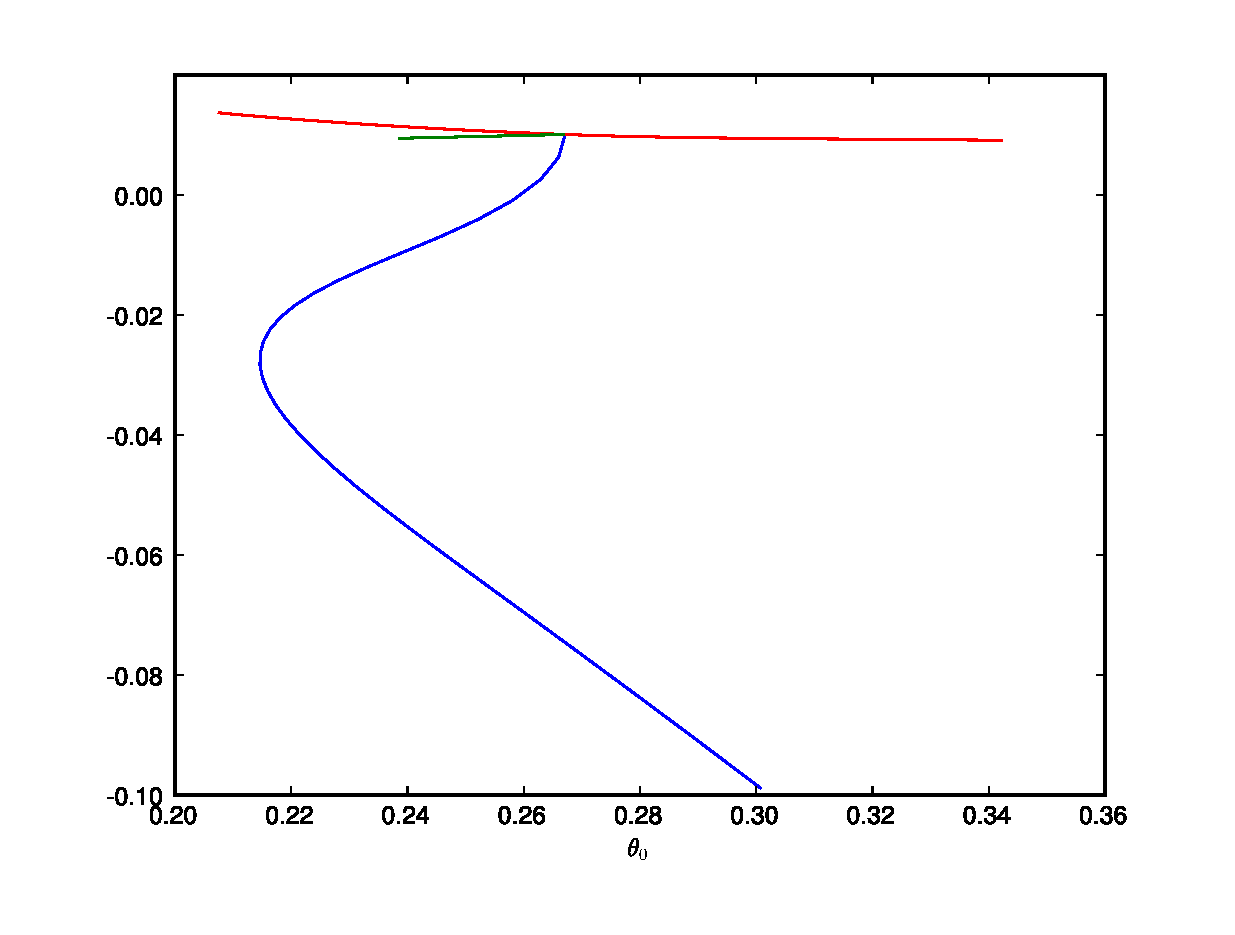
\includegraphics[scale=0.6]{Figuras/Lynx_controles_th1s.eps}
    \caption{$\theta_{1s}$ frente a $\theta_0$}
\end{figure}

\begin{figure}
	\includegraphics[scale=0.6]{Figuras/Lynx_controles_th1c.eps}
    \caption{$\theta_{1c}$ frente a $\theta_0$}
\end{figure}

Como se ve, es imposible satisfacer autom�ticamente todas las condiciones, as�
que hacemos lo siguiente:
\begin{enumerate}
    \item Ajustamos $\theta_0 = a + b\eta_{0p}$, para ello podemos exigir
        que por ejemplo el helic�ptero se encuentre en vuelo a punto 
        fijo para un 60\% de colectivo del piloto, es decir:
        \begin{align*}
            \eta_{0p} &= 0.6 & \theta_0 &= 0.239
        \end{align*}
        y que cubramos todo el margen de operaci�n del helic�ptero:
        \begin{align*}
            \eta_{0p} &= 0 & \theta_0&\leq 0.207 \\
            \eta_{0p} &= 1 & \theta_0&\geq 0.342
        \end{align*}

        Las anteriores condiciones se traducen en:
        \begin{align*}
            a &= 0.239 - 0.6b \\
            b &\geq 0.2575 
        \end{align*}

        Dando un poco de margen al final tenemos:
        \begin{equation*}
            \theta_0 = 0.059 + 0.3\eta_{0p}
        \end{equation*}
    \item Ajustamos los c�clicos en la forma:
        \begin{align*}
            \theta_{1s} &= a_s + b_s\eta_{0p} + c_s\eta_{1s} \\
            \theta_{1c} &= a_c + b_c\eta_{0p} + c_c\eta_{1c}
        \end{align*}
        para que sean en vuelo a punto fijo sea $\eta_{1sp} = \eta_{1cp} = 0$.
        Los c�clicos apenas var�an con $\theta_0$ as� que hacemos:
        \begin{equation*}
            a_s =  b_s = a_c = b_c = 0
        \end{equation*}
        Y damos una sensibilidad razonable a los controles:
        \begin{equation*}
            c_s = c_c = 0.2
        \end{equation*}

    \item Ajustamos el colectivo de cola de la misma forma que en los apartados 
        anteriores y queda:
        \begin{equation*}
            \theta_{0_T} = -0.061 + 0.441\eta_{0p} + 0.1\eta_{pp}
        \end{equation*}
\end{enumerate}

A falta de mejores datos los valores para el control autom�tico se han colocado
por prueba y error para dar un manejo m�s o menos sencillo del helic�ptero.

\section{Fichero de entrada}
A continuaci�n se muestra c�mo queda el fichero de entrada para el helic�ptero Lynx.
Guardar�amos el siguiente texto en un fichero de nombre \verb!Lynx.py! y lo
cargar�amos con el par�metro \verb!--modelo=Lynx!

\subsection{Pre�mbulo}
Todos los ficheros deben de incluir �ste pre�mbulo. Hay que tener en cuenta que
los ficheros de definici�n de los helic�pteros son ficheros de c�digo fuente en
python. Esto no quiere decir que sea necesario dominar el lenguaje ya que el
formato del fichero de entrada es suficientemente simple como para que no sea
necesario. Basta con utilizar un fichero de ejemplo y sustituir los valores
num�ricos correspondientes. Los casos mas complejos como la introducci�n de
matrices, tablas para interpolaciones, etc\ldots se cubren m�s adelante.

\begin{Verbatim}[frame=single,framerule=1mm]
# -*- coding: latin-1 -*-
#!!!!!!!!!!!!!!!!!!!!!!!!!!!!!!!!!!!!!!!!!!!!!!!!!!!!!
#			NO TOCAR 		
from modelo import Modelo
from matematicas import *
from numarray import *
from util import *
from integrador import *

import logging

modelo = Modelo()
#!!!!!!!!!!!!!!!!!!!!!!!!!!!!!!!!!!!!!!!!!!!!!!!!!!!!!
\end{Verbatim}

\subsection{Nombre}
El nombre del helic�ptero no es transcendente, sirve solo para mostrar por
pantalla ciertos mensajes haciendo referencia al helic�ptero. Como se ve el
nombre del helic�ptero es una cadena de texto, por lo que debe ir entre comillas
dobles o comillas simples:

\begin{Verbatim}[frame=single,framerule=1mm]
modelo.nombre = "Lynx"
\end{Verbatim}

\subsection{Integrador}
El integrador a utilizar. Los integradores disponibles se encuentran disponibles
en el fichero \verb!integrador.py!. Para asignar el integrador se escribe el
nombre y se acompa�a de dos par�ntesis al final. Los integradores disponibles
son:
\begin{itemize}
	\item Euler
	\item AdamsBashforth2
    \item RungeKutta4
    \item AdamsBashforth3
    \item ABM2
\end{itemize}

\begin{Verbatim}[frame=single,framerule=1mm]
modelo.integrador = AdamsBashforth2()
\end{Verbatim}

\subsection{Datos m�sicos del helic�ptero}
La masa del helic�ptero en kilogramos y los
momentos de inercia en kilogramos por metro al cuadrado. Se supone que el
helic�ptero es sim�trico respecto al plano xz por lo que la matriz de inercia es
de la forma:

\begin{equation}
	I = \left[\begin{array}{ccc}
		I_{xx} & 0 & -I_{xz} \\
		0 & I_{yy} & 0 \\
		-I_{xz} & 0 & I_{zz}
	\end{array}\right]
\end{equation}

\begin{Verbatim}[frame=single,framerule=1mm]
modelo.M = 4313.7		
modelo.Ixx = 2767.1		
modelo.Iyy = 13904.5		
modelo.Izz = 12208.8		
modelo.Ixz = 2034.8		
\end{Verbatim}

\subsection{Rotor principal}
\subsubsection{Posici�n y orientaci�n del rotor}
\begin{itemize}
	\item \verb!gas! ($\gamma_s$): Es la inclinaci�n del rotor positiva 
		hacia delante. Debe darse en radianes. En este caso se sabe que
		la inclinaci�n es de cuatro grados por lo que se utiliza la
		funci�n \verb!rad! que pasa de radianes a grados.
		Alternativamente se podr�a haber calculado aparte el �ngulo en
		radianes e introducirlo directamente.
		
	\item \verb!hR! ($h_R$): Distancia vertical del rotor al centro de
		masas, en metros. Evidentemente positiva con el rotor por encima
		del centro de masas.
	\item \verb!xcg! ($x_{cg}$): Distancia horizontal del rotor al centro de
		masas. Positiva cuando el rotor queda por detr�s del centro de
		masas. Unidades en metros.
	\item \verb!h0! ($h_0$): Distancia desde el rotor hasta el suelo en
		metros. 
\end{itemize}

\begin{Verbatim}[frame=single,framerule=1mm]
modelo.rotor.gas = rad(4)	
modelo.rotor.hR = 1.274		
modelo.rotor.xcg = -0.0198	
modelo.rotor.h0 = 2.946		
\end{Verbatim}

\subsubsection{Descripci�n geom�trica y m�sica del rotor}
\begin{itemize}
	\item \verb!Nb! ($N_b$): N�mero de palas del rotor. Actualmente las
		ecuaciones del rotor s�lo son correctas para cuatro palas.
	\item \verb!R! ($R$): Radio del rotor en metros.
	\item \verb!c! ($c$): Cuerda de los perfiles del rotor en metros.
	\item \verb!Ibe! ($I_\beta$): Momento de inercia en kilogramos por metro
		cuadrado de cada una de las palas del rotor respecto al eje de
		batimiento. 
	\item \verb!Kbe! ($K_\beta$): Muelle equivalente para el batimiento de
		la pala, en Newtons por radi�n. Se puede obtener a partir de la
		primera frecuencia de batimiento.
	\item \verb!tht! ($\theta_t$): Torsi�n lineal de la pala en radianes,
		por tanto torsi�n en la punta de la pala. Es decir, se supone que
		el paso de los perfiles de la pala debido a la torsi�n es del tipo:
		\begin{equation}
			\theta = \theta_t\frac{r}{R}
		\end{equation}
\end{itemize}

\begin{Verbatim}[frame=single,framerule=1mm]
modelo.rotor.Nb = 4		
modelo.rotor.R = 6.4		
modelo.rotor.c = 0.391		
modelo.rotor.Ibe = 678.14	
modelo.rotor.Kbe = 166352	
modelo.rotor.tht = -0.14	
\end{Verbatim}

\subsubsection{Descripci�n aerodin�mica de los perfiles de la pala}
\begin{itemize}
	\item \verb!a0! ($a_0$): pendiente de sustentaci�n de los perfiles.
		Se supone sim�trico, lineal e independiente del n�mero de Mach.
		Evidentemente como si depende del n�mero de Mach se selecciona
		la pendiente de sustentaci�n de una secci�n caracter�stica de la
		pala, por ejemplo la secci�n $\frac{3}{4}$.

	\item \verb!de0! ($\delta_0$)
	\item \verb!de1! ($\delta_1$)
	\item \verb!de2! ($\delta_2$): T�rminos de la polar de resistencia del
		perfil (adimensionales), no en funci�n del �ngulo de ataque, sino en funci�n del
		coeficiente de sustentaci�n del rotor principal. Es decir, el
		coeficiente de sustentaci�n de todos los perfiles del rotor se
		supone de la forma:
		\begin{equation}
			\delta = \delta_0 + \delta_1 c_T + \delta_2 c_T^2
		\end{equation}
		Se pueden calcular a partir de la polar cl�sica dada en funci�n
		del �ngulo de ataque de forma que el par del rotor sea el mismo.
\end{itemize}

\begin{Verbatim}[frame=single,framerule=1mm]
modelo.rotor.a0 = 6.0		
modelo.rotor.de0 = 0.009	
modelo.rotor.de1 = 0.0
modelo.rotor.de2 = 37.983	
\end{Verbatim}

\subsection{Rotor de cola}
\subsubsection{Posici�n y orientaci�n}

\begin{itemize}
	\item \verb!hT! ($h_T$): distancia vertical en metros del rotor de cola
		al centro de masas. Positiva con el rotor de cola por encima del
		centro de masas.
	\item \verb!lT! ($l_T$): distancia horizontal entre el rotor principal y
		el rotor de cola, en metros.
	\item \verb!K! ($K$): inclinaci�n del rotor de cola en radianes.
		Positivo seg�n un giro por el eje $-x$.
\end{itemize}
\begin{Verbatim}[frame=single,framerule=1mm]
modelo.rotor_cola.hT = 1.146		
modelo.rotor_cola.lT = 7.66		
modelo.rotor_cola.K = 0.0		
\end{Verbatim}

\subsubsection{Descripci�n geom�trica y m�sica}

\begin{itemize}
	\item \verb!RT! ($R_T$): radio del rotor de cola en metros.
	\item \verb!cT! ($c_T$): cuerda del rotor de cola en metros.
	\item \verb!IbeT! ($I_{\beta_T}$): momento de inercia en kilogramos por
		metro cuadrado de cada pala del rotor de cola respecto a su eje de
		batimiento.
	\item \verb!KbeT! ($K_{\beta_T}$): muelle equivalente del rotor de cola,
		en newtons por radi�n.
	\item \verb!k3! ($k_3$): Factor de acoplamiento entre el �ngulo de
		batimiento y el �ngulo de paso. Adimensional.
		\begin{align}
			\theta =& k_3\beta \\
			k_3 =& \tan \delta_3 \\
		\end{align}
	\item \verb!tht! ($\theta_{t_T}$): torsi�n lineal del rotor de cola.
	\item \verb!gT! ($g_T$): relaci�n entre la velocidad angular del rotor
		de cola y del rotor principal. Adimensional. 
		\begin{equation}
			g_T = \frac{\Omega_T}{\Omega}
		\end{equation}
\end{itemize}

\begin{Verbatim}[frame=single,framerule=1mm]
modelo.rotor_cola.RT = 1.106		
modelo.rotor_cola.cT = 0.18001		
modelo.rotor_cola.IbeT = 1.08926	
modelo.rotor_cola.KbeT = 2511.24	
modelo.rotor_cola.k3 = -1.		
modelo.rotor_cola.tht = 0.0 		
modelo.rotor_cola.gT = 5.8		
\end{Verbatim}

\subsubsection{Descripci�n aerodin�mica}
\begin{itemize}
	\item \verb!a0T! ($a_{0_T}$): pendiente de sustentaci�n de los perfiles
		del rotor de cola, con las mismas hip�tesis del rotor principal.
	\item \verb!de0T!
	\item \verb!de1T!
	\item \verb!de2T!: coeficientes de la polar de resistencia de los
		perfiles del rotor de cola, en funci�n del coeficiente de
		sustentaci�n del rotor de cola:
		\begin{equation}
			\delta = \delta_{0_T} + \delta_{1_T}c_{T_T} +
			\delta_{2_T}c_{T_T}^2
		\end{equation}
\end{itemize}
\begin{Verbatim}[frame=single,framerule=1mm]
modelo.rotor_cola.a0T = 6.0		
modelo.rotor_cola.de0T = 0.008		
modelo.rotor_cola.de1T = 0.0
modelo.rotor_cola.de2T = 5.334		
\end{Verbatim}

\subsection{Fuselaje}
\subsubsection{Descripci�n geom�trica}
\begin{itemize}
	\item \verb!Ss! ($S_s$): �rea lateral de fuselaje en metros cuadrados.
	\item \verb!Sp! ($S_p$): �rea frontal de fuselaje en metros cuadrados.
		Tanto $S_s$ como $S_p$ no necesitan ser los valores exactos, sino
		tan s�lo los valores de superficie que se han utilizado para 
		adimensionalizar los coeficientes $c_Y$, $c_l$, $c_m$ y $c_D$,
		$c_L$, $c_m$ respectivamente.
	\item \verb!lf! ($l_f$): longitud del fuselaje en metros. De nuevo basta con que
		sea la longitud utilizada en la adimensionalizaci�n de los
		coeficientes de momento.
	\item \verb!xca! ($x_{ca}$): posici�n horizontal del centro aerodin�mico
		del fuselaje, positivo por delante del centro de masas. En
		metros.
	\item \verb!zca! ($z_{ca}$): posici�n vertical del centro aerodin�mico,
		positivo debajo del centro de masas. En metros.
	\item \verb!ht! ($h_t$): distancia del centro de masas al suelo.
\end{itemize}
\begin{Verbatim}[frame=single,framerule=1mm]
modelo.fuselaje.Ss = 32.	
modelo.fuselaje.Sp = 24.	
modelo.fuselaje.lf = 12.
modelo.fuselaje.xca = 0.139
modelo.fuselaje.zca = 0.190	
modelo.fuselaje.ht = 1.67
\end{Verbatim}

\subsubsection{Coeficientes aerodin�micos del fuselaje}

La descripci�n aerodin�mica del fuselaje es la que presenta la estructura m�s
compleja de todo el archivo del modelo. Para empezar existen dos m�todos de
describir el fuselaje, denominados FuselajeA y FuselajeB. Para utilizar cada uno
de ellos se utiliza una de las dos opciones siguientes:

\begin{Verbatim}[frame=single,framerule=1mm]
modelo.fuselaje.aero = FuselajeA(
	...
)
\end{Verbatim}
o bien:

\begin{Verbatim}[frame=single,framerule=1mm]
modelo.fuselaje.aero = FuselajeB
	...
)
\end{Verbatim}

FuselajeB es el m�todo con la sintaxis m�s sencilla y el que presenta mayor
generalidad ya que s�lo requiere que se le pase una funci�n v�lida de python que
acepte como argumentos el �ngulo de ataque y el �ngulo de resbalamiento del
fuselaje y devuelve una tupla con los 6 coeficientes aerodin�micos: $c_D$,
$c_L$, $c_Y$, $c_l$, $c_m$, $c_n$ (en este orden). Evidentemente es un m�todo
que requiere un conocimiento m�s profundo de programaci�n en python. Por ello, y
porque a veces se tiene un conjunto reducido de datos sobre el fuselaje, se
proporciona el modelo de fuselaje A, que requiere �nicamente la sustituci�n de
los valores num�ricos de un fichero de ejemplo. Aunque para el helic�ptero Lynx
se utiliza el modelo de fuselaje A aqu� se muestra tambi�n el ejemplo del
BlackHawk:


\begin{Verbatim}[frame=single,framerule=1mm]
def aero(al, be):
	if al<-pi/2:
		al += pi
	elif al>pi/2:
		al -= pi
	if be<-pi/2:
		be += pi
	elif be>pi/2:
		be -= pi

	Sal, S2al, Sbe, S2be, S4be =\
		map(sin, [al, 2*al, be, 2*be, 4*be])
	Cal, C2al, Cbe, C2be, C4be =\
		map(cos, [al, 2*al, be, 2*be, 4*be])

	cD = 1.3944*(Sal)**2 - 0.6435*Cal + 2.4806 +\
	     0.0456*C4be - 1.597*C2be -\
	     8.2893e-9*(be**4)
	cL = 0.4546*Sal + 0.6730*S2al -\
	     1.2680*(Sal)**2 - 1.3029*Cal + 1.3215 +\
	     0.00127*be - 0.0465*S4be +\
	     0.0005*(be**2)
	cY = -0.0802*Sbe -0.1627*S2be + 0.0182*S4be
	
	if be<=rad(10):
		cl = 0.0
	elif rad(10)<be and be<=rad(25):
		cl = sign(be)*0.02098*(Cbe**4) - 0.0197
	else:
		cl = 0.0283*Sbe +\
		     sign(be)*(0.0022*C4be -\
		     0.0134*(Cbe)**3 +\
		     0.0338*(Cbe)**4 - 0.0308)
	
	cm = 0.0007 + 0.2291*S2al + 0.1343*(Sal)**2 +\
	     0.1095*Cal - 0.1606*(Cbe)**3 + 0.0176
	
	if be<=rad(20):
		cn = 0.0128*S2be - 0.0195*S4be -\
		     8.4339e-5
	else:
		cn = -0.0101*S2be +\
		     sign(be)*(0.0309*(C4be**4) - 0.0197)
	
	return cD, cL, cY, cl, cm, cn

modelo.fuselaje.aero = FuselajeB(aero)
\end{Verbatim}

A continuaci�n se muestra el modelo de fuselaje tal como se usa en el modelo
Lynx. La sintaxis es un poco m�s complicada, pero como ventajas presenta que no
requiere saber programar en python y adem�s a partir de pocos datos
aerodin�micos calcula (de forma muy aproximada) los coeficientes aerodin�micos
para todo �ngulo de ataque. La sintaxis es de la forma:

\begin{Verbatim}[frame=single,framerule=1mm]
modelo.fuselaje,aero = FuselajeA(
	nombre1 = valor1,
	nombre2 = valor2,
	...
	nombreN = valorN
)

\end{Verbatim}

Y el listado tal como aparece en el fichero del Lynx es, parte a parte:
\subsubsection{Declaraci�n del modelo de fuselaje}
\begin{Verbatim}[frame=single,framerule=1mm]
modelo.fuselaje.aero = FuselajeA( 
\end{Verbatim}

\subsubsection{Unidades}
Puede ser que los datos que se poseen del fuselaje den los coeficientes en
funci�n del �ngulo de ataque en grados. Como pasar dichos valores a radianes
puede ser muy pesado, se da la opci�n de introducir esos valores en grados o
radianes, con tal de que se indique en el fichero del modelo. En este caso se
utilizan grados, por lo que el valor que se le asigna \verb!unidades! es una
cadena de texto llamada \verb!deg!. Hay que notar que es una cadena de texto, por
lo que debe ir entre comillas dobles o simples.
\begin{Verbatim}[frame=single,framerule=1mm]
	unidades = 'deg',		
\end{Verbatim}
Si se hubiesen utilizado radianes se habr�a indicado:
\begin{Verbatim}[frame=single,framerule=1mm]
	unidades = 'rad',		
\end{Verbatim}
					
\subsubsection{Valores de los coeficientes para �ngulos de 90 grados}
\begin{Verbatim}[frame=single,framerule=1mm]
	cDa90 = 0.3480,			
	cDb90 = 0.4784,			
	cm90 =  0.03,			
	cl90 =  0.01,			
	cn90 =  0.1,			
\end{Verbatim}
\subsubsection{Rango de los �ngulos de ataque y resbalamiento para los cuales se
utilizan valores precisos}
Fuera de este rango se aproxima el valor de los coeficientes utilizando los
valores que anteriormente se han introducido para 90 grados. Como utilizamos
�ngulos en grados, estos valores van en grados.
\begin{Verbatim}[frame=single,framerule=1mm]
	al1 = -21,
	al2 =  21,
	
	be1 = -21,
	be2 =  21,
\end{Verbatim}
\subsubsection{Valores de los coeficientes para �ngulos peque�os}
La sintaxis es:

\begin{Verbatim}[frame=single,framerule=1mm]
	cDa = Lista(
		angulo1, valor1,
		angulo2, valor2,
		...
	),
	cDb = Lista(
		...
	),
	cm = Lista(
		...
	),
	cL = Lista(
		...
	),
	cl = Lista(
		...
	),
	cY = Lista(
		...
	),
	cn = Lista(
		...
	),
\end{Verbatim}
donde:
\begin{itemize}
	\item \verb!cDa! ($c_{D_\alpha}$): coeficiente de resistencia para
		�ngulo de resbalamiento nulo, en funci�n de �ngulo de ataque.
	\item \verb!cDa! ($c_{D_\beta}$): coeficiente de resistencia para
		�ngulo de ataque nulo, en funci�n de �ngulo de resbalamiento.
	\item \verb!cm! ($c_m$): coeficiente de momento de cabeceo en funci�n de
		�ngulo de ataque.
	\item \verb!cL! ($c_L$): coeficiente de sustentaci�n en funci�n de
		�ngulo de ataque.
	\item \verb!cl! ($c_l$): coeficiente de momento de balance, en funci�n
		de �ngulo de resbalamiento.
	\item \verb!cY! ($c_Y$): coeficiente de fuerza lateral, en funci�n
		de �ngulo de resbalamiento.
	\item \verb!cn! ($c_n$): coeficiente de momento de gui�ada, en funci�n
		de �ngulo de resbalamiento.
\end{itemize}
Y a continuaci�n el listado tal como se encuentra en el fichero del modelo del
Lynx. De nuevo expresamos los �ngulos en grados tal como se especific� en
\verb!unidades!. Tambi�n notamos la presencia de un par�ntesis al final que
cierra el par�ntesis que se abri� con \verb!FuselajeA(!

%\begin{Verbatim}[frame=single,framerule=1mm]
\begin{Verbatim}[frame=single,framerule=1mm]
	cDa = Lista(
		-21, 0.06661,
		-18, 0.06010,
		-15, 0.05531,
		-12, 0.04991,
		 -9, 0.04707,
		 -6, 0.04561,
		 -3, 0.04421,
		  0, 0.04233,
		  3, 0.04245,
		  6, 0.04372,
		  9, 0.04486,
		 12, 0.04685,
		 15, 0.04926,
		 18, 0.05170,
		 21, 0.05613 
	),
	
	cDb = Lista(
		-21, 0.05532,
		-18, 0.04096,
		-15, 0.02863,
		-12, 0.01842,
		 -9, 0.01040,
		 -6, 0.00464,
		 -3, 0.00116,
		  0, 0.00000,
		  3, 0.00116,
		  6, 0.00464,
		  9, 0.01040,
		 12, 0.01842,
		 15, 0.02863,
		 18, 0.04096,
		 21, 0.05532 
	),

	cm = Lista(
		-21, -0.02415,
		-18, -0.02210,
		-15, -0.02015,
		-12, -0.01803,
		 -9, -0.01588,
		 -6, -0.01351,
		 -3, -0.01074,
		  0, -0.00747,
		  3, -0.00421,
		  6, -0.00085,
		  9,  0.00237,
		 12,  0.00573,
		 15,  0.00875,
		 18,  0.01197,
		 21,  0.01433 
	),
	
	cL = Lista(
		-21, -0.02415,
		-18, -0.02210,
		-15, -0.02015,
		-12, -0.01803,
		 -9, -0.01588,
		 -6, -0.01351,
		 -3, -0.01074,
		  0, -0.00747,
		  3, -0.00421,
		  6, -0.00085,
		  9,  0.00237,
		 12,  0.00573,
		 15,  0.00875,
		 18,  0.01197,
		 21,  0.01433 
	),
		
	cY = Lista(	
		-21,  0.17547,
		-18,  0.15138,
		-15,  0.12677,
		-12,  0.10178,
		 -9,  0.07653,
		 -6,  0.05110,
		 -3,  0.02557,
		  0,  0.00000,
		  3, -0.02557,
		  6, -0.05110,
		  9, -0.07653,
		 12, -0.10178,
		 15, -0.12677,
		 18, -0.15138,
		 21, -0.17547 
	),
	
	cl = Lista(
		-21, -0.00697,
		-18, -0.00472,
		-15, -0.00270,
		-12, -0.00097,
		 -9,  0.00000,
		 -6,  0.00000,
		 -3,  0.00000,
		  0,  0.00000,
		  3,  0.00000,
		  6,  0.00000,
		  9,  0.00000,
		 12,  0.00097,
		 15,  0.00270,
		 18,  0.00472,
		 21,  0.00697 
	),
	
	cn = Lista(
		-21, -0.01704,
		-18, -0.01461,
		-15, -0.01217,
		-12, -0.00974,
		 -9, -0.00730,
		 -6, -0.00487,
		 -3, -0.00243,
		  0,  0.00000,
		  3,  0.00243,
		  6,  0.00487,
		  9,  0.00730,
		 12,  0.00974,
		 15,  0.01217,
		 18,  0.01461,
		 21,  0.01704
	)
)
\end{Verbatim}
%\end{Verbatim}
\subsection{Estabilizador horizontal}

\subsubsection{Posici�n y orientaci�n}
\begin{itemize}
	\item \verb!ltp! ($l_{tp}$): distancia horizontal desde el rotor al
		estabilizador horizontal en metros.
	\item \verb!htp! ($h_{tp}$): distancia vertical desde el centro de masas
		al estabilizador horizontal, positiva con el estabilizador
		horizontal por encima del centro de masas, en metros.
	\item \verb!S_{tp}! ($S_{tp}$): �rea del estabilizador horizontal en
		metros cuadrados.
	\item \verb!altp0! ($\alpha_{tp_0}$): �ngulo de ataque del estabilizador
		horizontal, con  helic�ptero sin �ngulo de ataque. En radianes.
\end{itemize}
\begin{Verbatim}[frame=single,framerule=1mm]
modelo.estabilizador_horizontal.ltp = 7.66			
modelo.estabilizador_horizontal.htp = 1.146			
modelo.estabilizador_horizontal.Stp = 1.197			
modelo.estabilizador_horizontal.altp0 = rad(-1.0)		
\end{Verbatim}
\subsubsection{Propiedades aerodin�micas}

De la misma forma que con el fuselaje tenemos varias posibilidades para elegir:
perfilA, perfilB, perfilC. La m�s general es el modelo de perfil C, ya que
permite especificar las dos funciones que para todo �ngulo de ataque devuelven
los coeficientes de resistencia y sustentaci�n. Su sintaxis es:

\begin{Verbatim}[frame=single,framerule=1mm]
	modelo.estabilizador_horizontal.aero = perfilC(
			cL = funcion_cL,
			cD = funcion_cD
	)
\end{Verbatim}

Donde \verb!funcion_cL! y \verb!funcion_cD! son funciones escritas en python que
aceptan un �nico valor, el �ngulo de ataque y devuelven un �nico valor, el
coeficiente que corresponda.

Para el fichero del modelo Lynx utilizamos el modelo de perfil A, que es el
recomendado. El significado de los par�metros que intervienen es:
\begin{itemize}
	\item \verb!AR! ($A$): alargamiento del estabilizador. 
	\item \verb!a! ($a$): pendiente de sustentaci�n.
	\item \verb!cLmax! ($c_{L_{max}}$): m�ximo coeficiente de sustentaci�n.
	\item \verb!de0! ($\delta_0$)
	\item \verb!de1! ($\delta_1$)
	\item \verb!de2! ($\delta_2$): coeficientes de la polar del perfil, para
		obtener el coeficiente de resistencia del perfil en funci�n del
		�ngulo de ataque:
		\begin{equation}
			c_D = \delta_0 + \delta_1\alpha + \delta_2\alpha^2
		\end{equation}
\end{itemize}

\begin{Verbatim}[frame=single,framerule=1mm]
modelo.estabilizador_horizontal.aero = perfilA(			
		AR  =  2.7, 		
		a   =  2.3663,		
		cLmax = 0.6,		
		de0 =  1.065e-3,	
		de1 = -8.4703e-2,	
		de2 =  1.46981
)
\end{Verbatim}

Si no se obtienen datos suficientes del perfil se puede indicar �nicamente el
alargamiento y el programa calcular� autom�ticamente el resto de par�metros. Por
ejemplo, si hubi�semos hecho:

\begin{Verbatim}[frame=single,framerule=1mm]
modelo.estabilizador_horizontal.aero = perfilA(			
		AR  =  2.7, 		
\end{Verbatim}

los otros par�metros habr�an sido calculados autom�ticamente.

\subsection{Controles}

\begin{itemize}
	\item \verb!c0! ($\vec{c}_0$): pasos del rotor para controles nulos.
	\item \verb!c1! ($c_1$): sensibilidad y mezcla de los controles.
	\item \verb!S0! ($S_0$)
	\item \verb!S1! ($S_1$)
	\item \verb!S2! ($S_2$): matrices para el sistema de control autom�tico.
    \item \verb!th_0! ($\theta_0$): cabeceo marcado por el sistema de control. 
        Se puede especificar como una constante o como una funci�n del mando
        longitudinal.
    \item \verb!fi_0! ($\phi_0$): balance marcado por el sistema de control. 
        Se puede especificar como una constante o como una funci�n del mando
        lateral.
    \item \verb!ch_0! ($\psi_0$): gui�ada marcada por el sistema de control.
        Se puede especificar como una constante o como una funci�n de los pedales.
	\item \verb!L! ($L$): l�mite del sistema autom�tico de control.
\end{itemize}

\begin{Verbatim}[frame=single,framerule=1mm]
modelo.controles.c0 = array([ 
              0.059,    
              0.000,    
              0.000, 
             -0.061, 
            ], type='Float64')


modelo.controles.c1 = array([
            [ 0.300, 0.000,  0.000,  0.000 ],
            [ 0.000, 0.200,  0.000,  0.000 ],
            [ 0.000, 0.000,  0.200,  0.000 ],
            [ 0.441, 0.000,  0.000,  0.100 ],
            ], type='Float64')

modelo.controles.S0 = array([
    [ 1.0000, 0.0000, 0.0000, 0.0000 ],
    [ 0.0000, 0.0000, 0.0000, 0.0000 ],
    [ 0.0000, 0.0000, 0.0000, 0.0000 ],
    [ 0.0000, 0.0000, 0.0000, 1.0000 ]], type='Float64')

modelo.controles.S1 = array([
    [ 0.0000,  0.0000, 0.0000 ],
    [ 0.0000, -2.5000, 0.0000 ],
    [ 2.5000,  0.0000, 0.0000 ],
    [ 0.0000,  0.0000, 0.6000 ]], type='Float64')

modelo.controles.S2 = array([
    [  0.0000,  0.0000, 0.0000 ],
    [ -2.5000,  0.0000, 0.0000 ],
    [  0.0000,  2.5000, 0.0000 ],
    [  0.0000,  0.0000, 0.0000 ]], type='Float64')

modelo.controles.th_0 =  lambda et1sp:  0.0603 + 1.4*et1sp
modelo.controles.fi_0 =  lambda et1cp: -0.0476 - 1.4*et1cp
modelo.controles.ch_0 =  0.0

modelo.controles.L = 0.2
\end{Verbatim}

Para introducir funciones se recuerda que puede ser cualquier tipo de codigo
en python v�lido, y tambi�n se pueden especificar mediante listas, de forma 
que se podr�a haber escrito (y hubiese sido equivalente):
\begin{Verbatim}[frame=single,framerule=1mm]
modelo.controles.th_0 = Lista( 0,  0.0603,
                               1,  1.4603 )
modelo.controles.fi_0 = Lista( 0, -0.0476,
                               1, -1.4476 )
\end{Verbatim}

\subsection{Motor}
\begin{itemize}
    \item \verb!n! ($n$): N�mero de motores.
	\item \verb!Omi! ($\Omega_i$): Velocidad nominal de rotaci�n del rotor.
    \item \verb!Wto! ($W_{to_0}$): M�xima potencia de despegue a nivel del mar.
    \item \verb!Wmc! ($W_{mc_0}$): M�xima potencia continua a nivel del mar.
    \item \verb!x! ($x$): Coeficiente de variaci�n de potencia disponible con la
        altura.
    \item \verb!Wid! ($W_{id}$): M�nima potencia de operaci�n del motor.
    \item \verb!K_3! ($K_3$): rigidez del motor.
    \item \verb!P! ($P$): P�rdidas del sistema de transmisi�n del rotor y rotor de cola.
    \item \verb!Irt! ($I_R$): Inercia del sistema de transmisi�n en funci�n del
        n�mero de motores activos.
    \item \verb!tae1! ($\tau_1$): Primera constante de tiempos del motor.
    \item \verb!a2! ($a_2$)
    \item \verb!b2! ($b_2$)
    \item \verb!c2! ($c_2$): Par�metros para la segunda constante de tiempos del 
        motor $\tau_2$.
    \item \verb!a3! ($a_3$)
    \item \verb!b3! ($b_3$)
    \item \verb!c3! ($c_3$): Par�metros para la tercera constante de tiempos del 
        motor $\tau_3$.
\end{itemize}

\begin{Verbatim}[frame=single,framerule=1mm]

modelo.motor.Omi = 35.63        
                                
modelo.motor.Wto_0 = 746000       
modelo.motor.Wmc_0 = 664000
modelo.motor.x     = 0.85
modelo.motor.Wid   = 1000         

modelo.motor.K3 = 65e3          

modelo.motor.n = 2              
modelo.motor.P  = 0.1           
                    
modelo.motor.Irt = [            
                3085.069,       
                3344.716,       
                3344.716]       

modelo.motor.tae1 = 0.1

modelo.motor.a2 = 0.1
modelo.motor.b2 = 0.1
modelo.motor.c2 = 0.1

modelo.motor.a3 = 0.1
modelo.motor.b3 = 0.1
modelo.motor.c3 = 0.1
\end{Verbatim}

\section{Trimado}
A continuaci�n se comentan resultados de trimado del Lynx, a partir de los
cuales se comenta sobre la validez del modelo.

\subsection{Vuelo a punto fijo}
A continuaci�n se presenta la posici�n de colectivo necesaria para mantener
vuelo a punto fijo a diferentes alturas sobre el suelo y la variaci�n del 
resto de los controles con el el colectivo.

Como se puede ver en la gr�fica \ref{fig:colectivo altura}, el colectivo (en radianes) 
var�a con la altura (en metros) debido al efecto suelo. Para valores mayores al radio 
del rotor el efecto suelo apenas se nota. La verdadera distancia del rotor al suelo 
es la altura de la figura ($z$) m�s la altura del fuselaje ($h_0=2.496m$)

\begin{figure}
	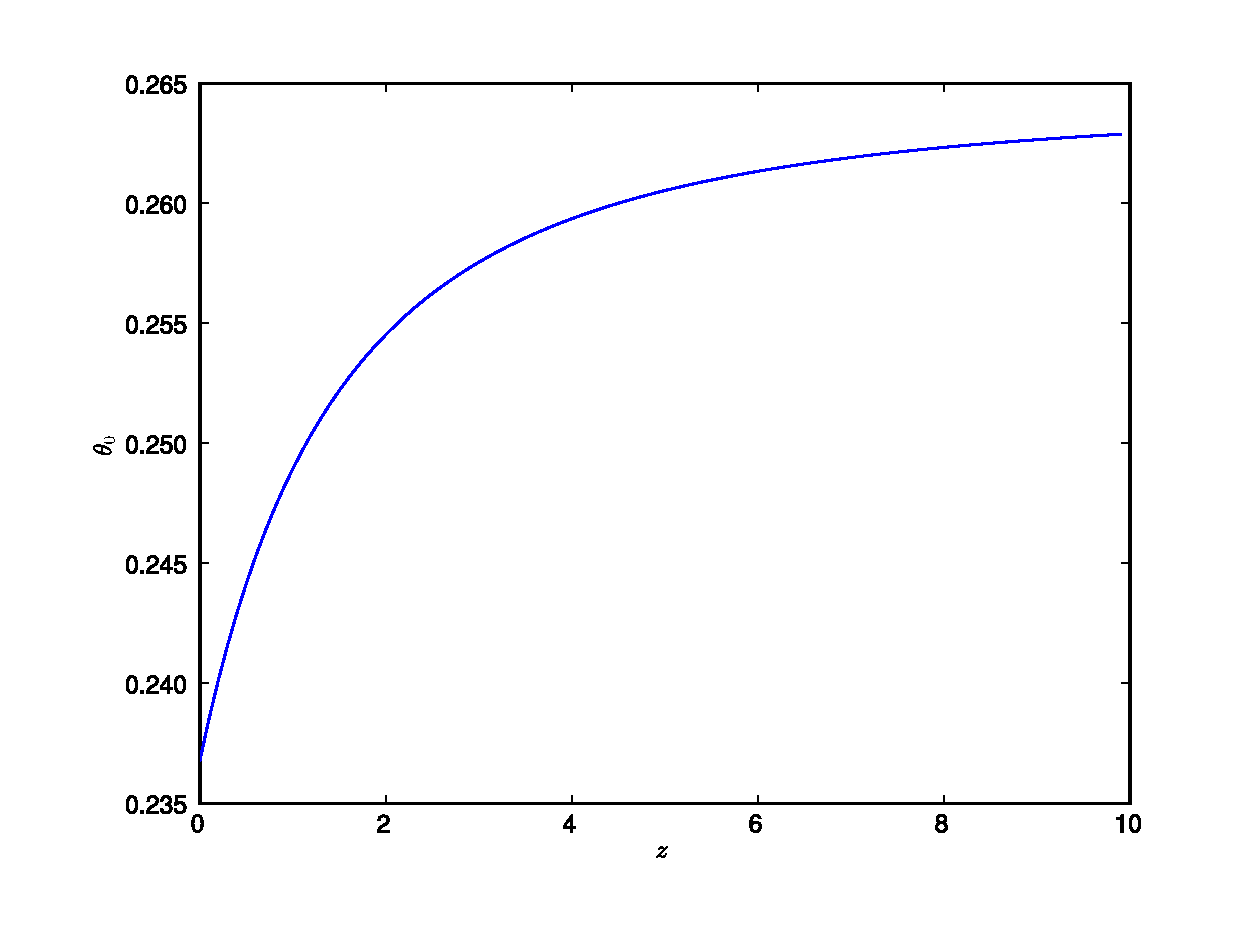
\includegraphics[width=12cm]{Figuras/trim_th0_z.eps}
	\caption{Colectivo en funci�n de la altura}
    \label{fig:colectivo altura}
\end{figure}

Para determinar los valores de las ganancias de los mandos calculamos la
variaci�n de $\theta_{0_T}$, $\theta_{1c}$ y $\theta_{1s}$ con el colectivo.
Como podemos ver $\theta_{1s}$ no es exactamente cero debido al peque�o
desplazamiento del centro de masas respecto al centro del rotor, por lo que
necesita compensar el ligero momento que se produce. El a�n m�s peque�o valor de
$\theta_{1c}$ es debido al acoplamiento lateral-longitudinal de la respuesta de
del helic�ptero, o dicho de otro modo, debido a que la frecuencia de batimiento
de las palas no es exactamente la de giro del rotor, el desfase entre el paso y
el batimiento no es exactamente de 90�, por lo que se produce ese peque�o
acoplamiento.

\begin{figure}
	\includegraphics[width=12cm]{Figuras/trim_th0T_th0.eps}
	\caption{Colectivo de cola en funci�n de colectivo}
\end{figure}

\begin{figure}
	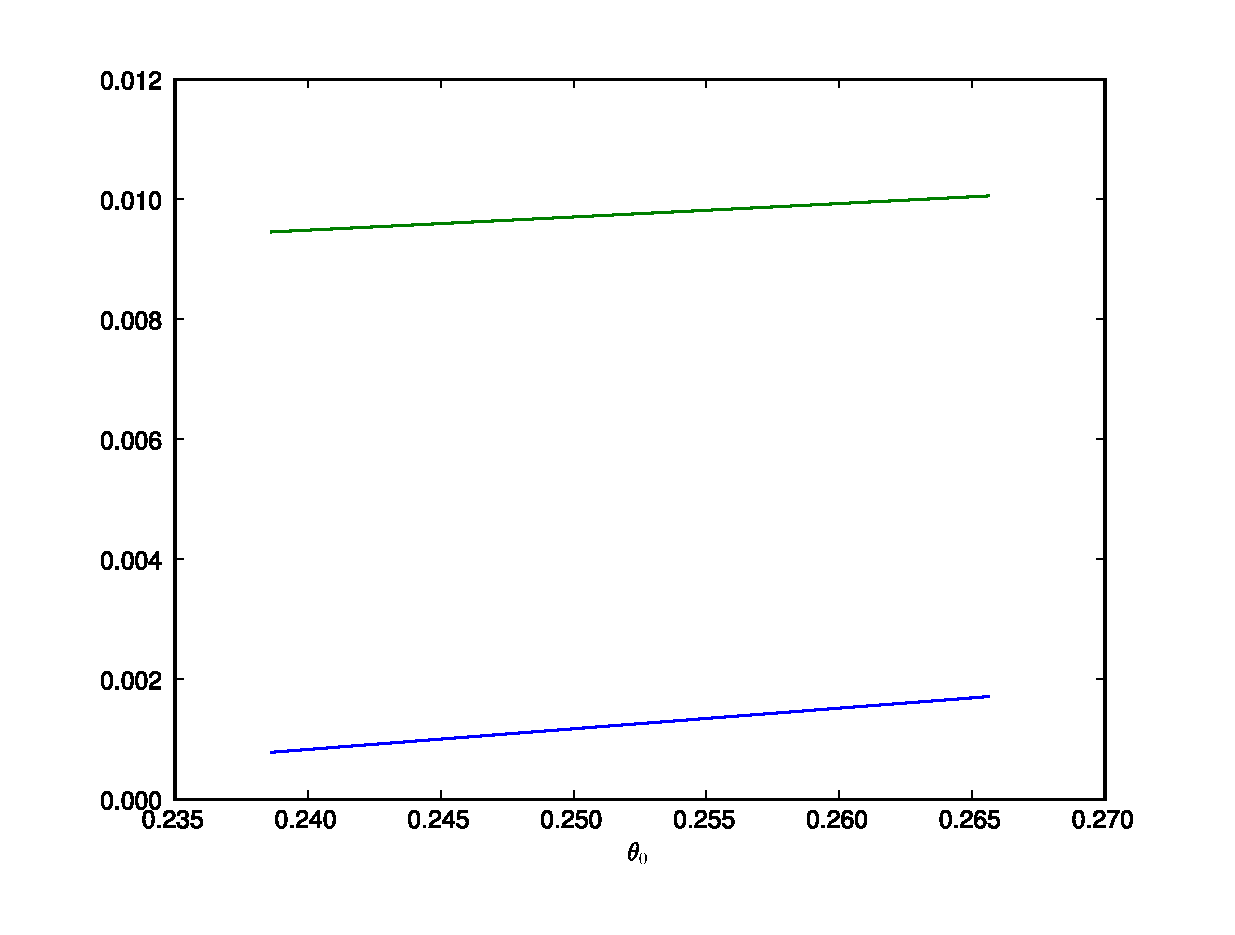
\includegraphics[width=12cm]{Figuras/trim_th1c_th1s_th0.eps}
	\caption{C�clico en funci�n de colectivo}
\end{figure}

\subsection{Efecto suelo}

A continuaci�n se presenta la variaci�n del efecto suelo para diferentes
velocidades, de 0 a 25m/s, y alturas, de 0 a 10m. Como se puede ver, al aumentar
la velocidad disminuye en general el requerimiento de colectivo pero tambi�n los
beneficios del efecto suelo. Para los primeros 10 m/s ambos efectos se cancelan,
lo cual es afortunado porque permite realizar una transici�n sencilla desde
punto fijo a vuelo en avance en las cercan�as del suelo.

\begin{figure}
	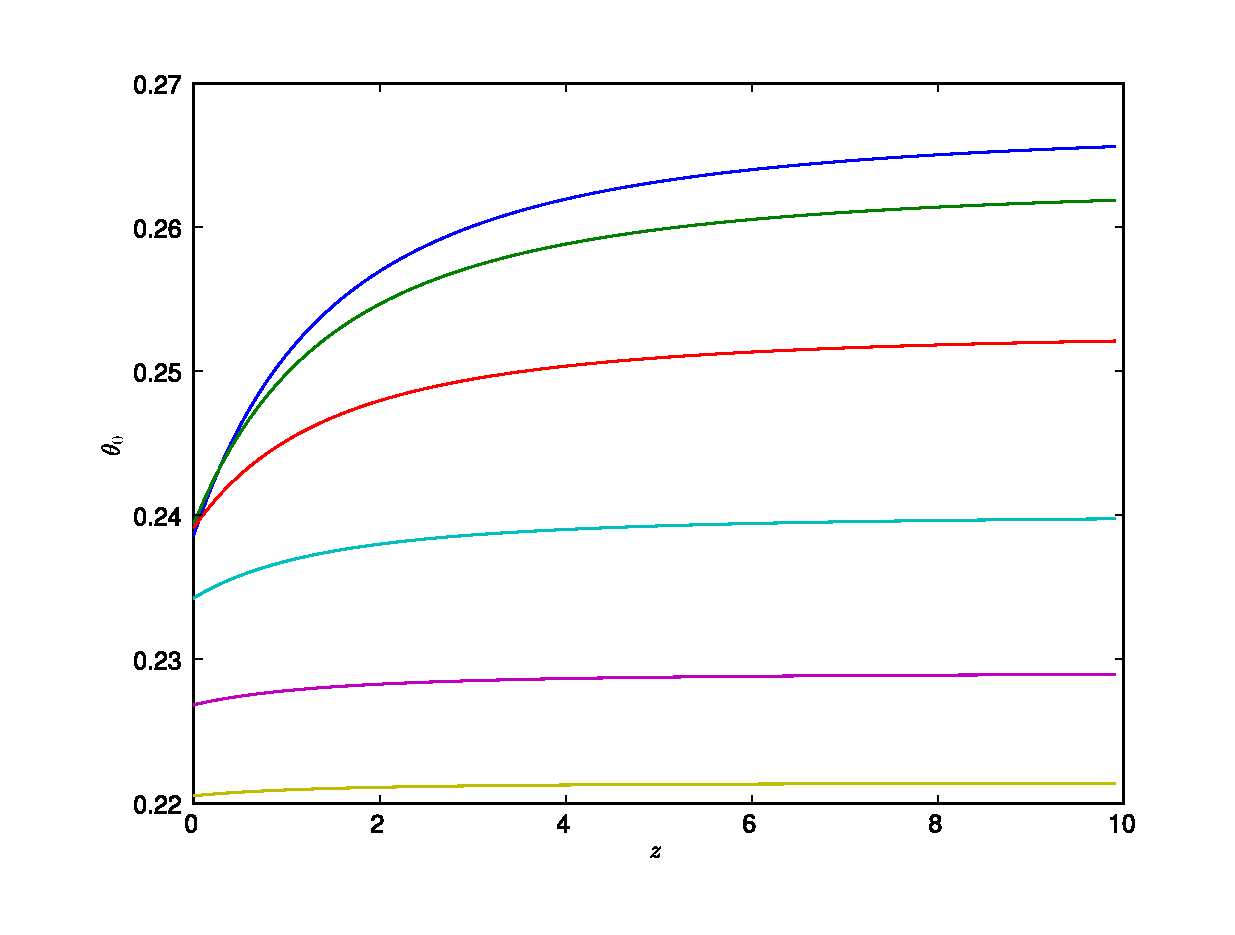
\includegraphics[width=12cm]{Figuras/trim_th0_V_z.eps}
	\caption{Colectivo en funci�n de velocidad y altura}
\end{figure}

\subsection{Vuelo vertical}
A continuaci�n (figura \ref{fig:velocidad velocidad ascensional}) se muestran 
resultados para diferentes velocidades 
ascensionales $V_a (m/s)$, en ausencia de efecto suelo. Se puede apreciar en la
gr�fica de la velocidad inducida frente a velocidad ascensional como al haber
aplicado la TCMM tenemos una transici�n suave desde el r�gimen de vuelo a punto
fijo hasta molinete frenante, pasando por autorrotaci�n.

\begin{figure}
	\includegraphics[width=12cm]{Figuras/trim_la0_Va.eps}
	\caption{Velocidad inducida frente a velocidad ascensional}
    \label{fig:velocidad velocidad ascensional}
\end{figure}

Para el vuelo vertical la expresi�n del coeficiente de sustentaci�n del rotor
es:
\[
c_T = \frac{a_0s}{2}\left[\frac{\theta_0}{3} + \frac{\mu_z-\lambda_0}{2} +
\frac{\theta_t}{4}\right] 
\]

Aproximadamente permanece $c_T$ constante, siendo la peque�a variaci�n debida a
la resistencia del fuselaje, por lo que $\theta_0$ var�a proporcionalmente a $\mu_z
- \lambda_0$, como se ve en la figura.

\begin{figure}
	\includegraphics[width=12cm]{Figuras/trim_th0_Va.eps}
	\caption{Colectivo frente a velocidad ascensional}
\end{figure}

Se puede despejar tambi�n $\theta_{0_T}$ en funci�n de $\theta_0$, pero la
relaci�n es bastante m�s complicada, lo importante es que como muestra la figura
la relaci�n no es lineal.

\begin{figure}
	\includegraphics[width=12cm]{Figuras/trim_th0T_th0_Va.eps}
	\caption{Colectivo de cola frente a colectivo para diferentes
	velocidades ascensionales}
\end{figure}


\subsection{Vuelo en avance}
Por �ltimo, el r�gimen mas com�n en la operaci�n del helic�ptero. Si no se especifica
nada se asume que los �ngulos se encuentran en radianes y la velocidad en nudos. 
Si todav�a hab�a esperanzas de encontrar unas ganancias de controles sencillas que nos
mantuviesen el helic�ptero cercano al trimado se desvanecen ahora, ya que
observando la posici�n del colectivo frente a la velocidad 
(figura \ref{fig:colectivo velocidad avance}) vemos que hay el
mismo colectivo para diferentes velocidades. El motivo es que seg�n aumenta la
velocidad del helic�ptero aumenta la eficiencia del rotor al empezar a
comportarse �ste de forma similar a un ala, por lo que para un mismo $c_T$
disminuye la necesidad de $\theta_0$, por lo que hay una tendencia inicial de
$\theta_0$ a bajar con la velocidad. Sin embargo, la resistencia del fuselaje y
del rotor aumenta tambi�n con la velocidad, de forma que esta tendencia
domina para velocidades altas, pero en alg�n punto entre velocidad nula y
velocidad alta se alcanza el m�nimo.

\begin{figure}
	\includegraphics[width=12cm]{Figuras/trim_th0_V.eps}
	\caption{Colectivo para diferentes velocidades de avance}
    \label{fig:colectivo velocidad avance}
\end{figure}

Siempre es conveniente comprobar que la velocidad inducida adopta la t�pica forma. 
En este caso vemos tambi�n como gracias al modelo de estela se predice correctamente
la velocidad no uniforme, ya que es aproximadamente:
\begin{equation*}
    \lambda_{1c} = \lambda_0\tan\frac{|\chi|}{2}
\end{equation*}
Donde $\chi$ es el �ngulo de la estela. Ver figura \ref{fig:inducida avance}.

\begin{figure}
	\includegraphics[width=12cm]{Figuras/trim_la0_la1c_V.eps}
    \caption{$\lambda_0$ y $\lambda_{1c}$ en funci�n de velocidad de avance}
    \label{fig:inducida avance}
\end{figure}

El otro control que m�s influye sobre el vuelo en avance es el c�clico
longitudinal, debido a que es necesario mantener inclinado el helic�ptero hacia
adelante para que la tracci�n del rotor compense la resistencia del fuselaje. El
cabeceo $\theta$ necesario queda muy bien aproximado entonces por
$\theta=-\frac{D}{Mg}$, por lo que, como se ve en la figura \ref{fig:cabeceo velocidad}, tiene una forma 
parab�lica.

\begin{figure}
	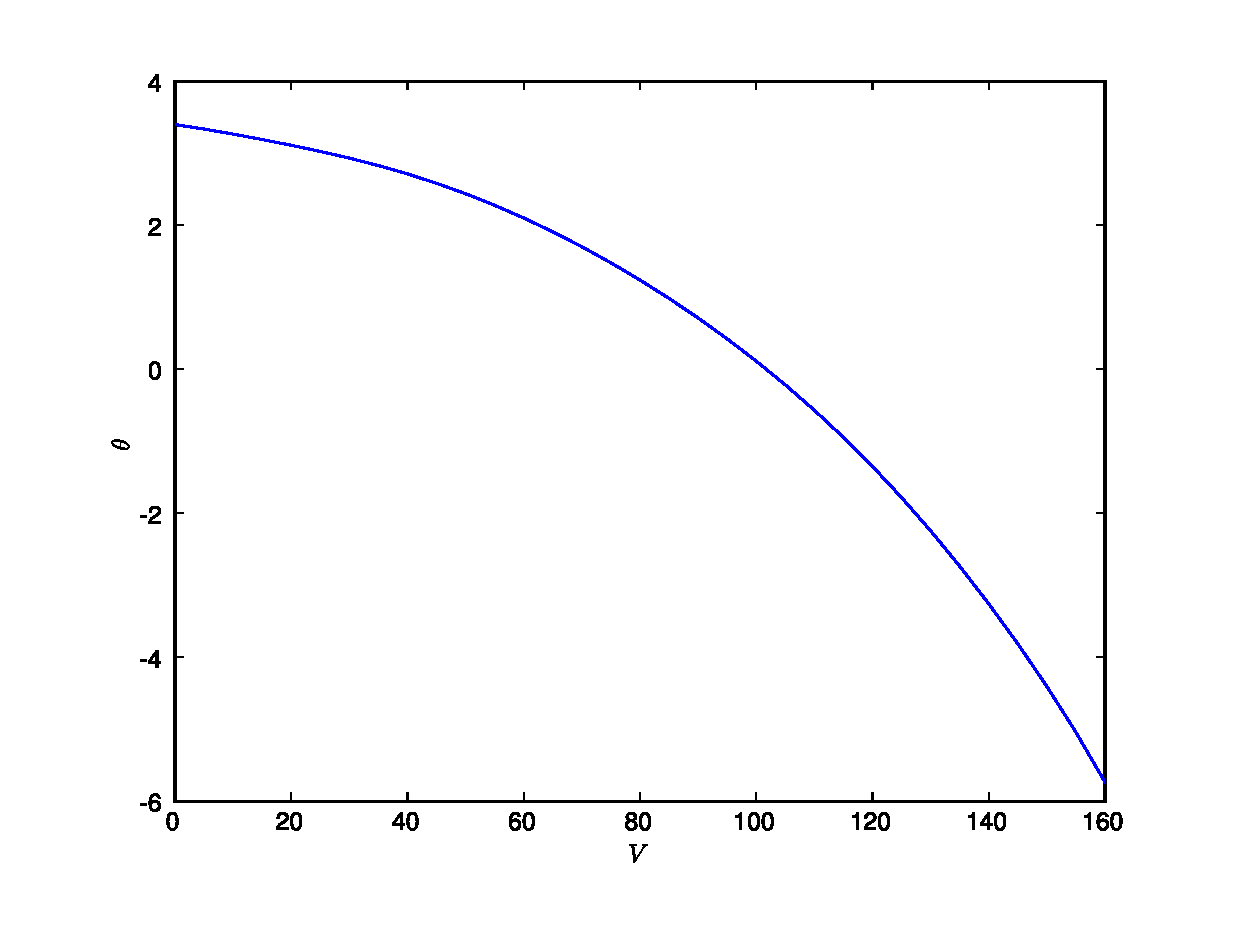
\includegraphics[width=12cm]{Figuras/trim_th_V.eps}
	\caption{Cabeceo en grados para diferentes velocidades de avance}
    \label{fig:cabeceo velocidad}
\end{figure}

Debido a la inestabilidad del momento del fuselaje, al aumentar el cabeceo
aumenta el momento aerodin�mico y por tanto tiene que aumentar el batimiento
longitudinal $\beta_{1c}$ para compensarlo; el aumento de este batimiento debido
al desfase cercano a 90� de paso y batimiento se advierte sobre todo en el c�clico 
$\theta_{1s}$. $\theta_{1c}$ no var�a demasiado y permanece peque�o gracias a
que a pesar de que el incremento de tracci�n del rotor de cola produce un
aumento de momento de balance, �ste se encuentra aproximadamente equilibrado por
el momento que se produce en el rotor de forma natural al aumentar la
diferencia de velocidades entre la pala que avanza y la pala que retrocede 
(figura \ref{fig:ciclicos avance}).

\begin{figure}
	\includegraphics[width=12cm]{Figuras/trim_th1c_th1s_V.eps}
	\caption{C�clicos para diferentes velocidades de avance}
    \label{fig:ciclicos avance}
\end{figure}

Vemos c�mo el �ngulo de balance $\phi$ sirve para compensar la fuerza
lateral de la cola, siendo su variaci�n exactamente opuesta (figura \ref{fig:balance cola avance}).

\begin{figure}
	\includegraphics[width=12cm]{Figuras/trim_cTT_fi_V.eps}
	\caption{Tracci�n de cola y �ngulo de balance frente a velocidad de
	avance}
    \label{fig:balance cola avance}
\end{figure}

Por �ltimo, se muestra el colectivo de cola frente a la velocidad de avance. Esta
curva est� determinada por dos factores: el comportamiento similar al colectivo
del rotor principal frente a la velocidad de avance y la necesidad de variar su
tracci�n como muestra la gr�fica de $c_{T_T}$ para compensar el par del rotor
principal (figura \ref{fig:cola avance}).

\begin{figure}
	\includegraphics[width=12cm]{Figuras/trim_th0T_V.eps}
	\caption{Colectivo de cola frente a velocidad de
	avance}
    \label{fig:cola avance}
\end{figure}

\subsection{Giro a nivel sin resbalamiento}
Para que no haya resbalamiento debe compensar la aceleraci�n centr�fuga a la
gravedad por lo que, como vemos en la figura \ref{fig:fi(Oma)}, es 
aproximadamente:
\begin{equation*}
    \phi = \arctan\frac{\Omega_aV}{g}
\end{equation*}

\begin{figure}
	\includegraphics[width=12cm]{Figuras/trim_fi_Oma.eps}
	\caption{Balance en funci�n de velocidad de giro}
    \label{fig:fi(Oma)}
\end{figure}

\begin{figure}
	\includegraphics[width=12cm]{Figuras/trim_th_Oma.eps}
	\caption{Cabeceo en funci�n de velocidad de giro}
\end{figure}

El colectivo tiene que compensar por la p�rdida de tracci�n vertical
al inclinar el helic�ptero y el colectivo de cola a su vez compensa
el par de rotor debido al aumento de colectivo.

\begin{figure}
	\includegraphics[width=12cm]{Figuras/trim_th0_Oma.eps}
	\caption{Colectivo en funci�n de velocidad de giro}
\end{figure}

\begin{figure}
	\includegraphics[width=12cm]{Figuras/trim_th0_Oma.eps}
	\caption{Colectivo de cola en funci�n de velocidad de giro}
\end{figure}

\begin{figure}
	\includegraphics[width=12cm]{Figuras/trim_th1c_th1s_Oma.eps}
	\caption{C�clicos en funci�n de velocidad de giro}
\end{figure}

\section{Derivadas de estabilidad}
A continuaci�n se presenta de forma gr�fica el c�lculo de las derivadas de
estabilidad a partir de cada situaci�n de trimado. En concreto se ha perturbado
en la velocidad, la velocidad angular y los controles un valor de $\pm 0.001$ y
se ha calculado la perturbaci�n correspondiente en cada una de las tres fuerzas y
tres momentos que act�an sobre el helic�ptero. Las fuerzas se encuentran
divididas por la masa del helic�ptero y los momentos por la inercia, teniendo
en cuenta el efecto de los momentos de inercia cruzados. De formas m�s exacta,
si la prima indica la magnitud antes de casi-adimensionalizar:

\begin{align}
	X =& \frac{X'}{M} \mbox{  } \left[\frac{m}{s^2}\right]\\
	Y =& \frac{Y'}{M} \mbox{  } \left[\frac{m}{s^2}\right]\\
	Z =& \frac{Z'}{M} \mbox{  } \left[\frac{m}{s^2}\right]\\
	L =& \frac{I_{zz}}{I_{xx}I_{zz} - I_{xz}^2}L' +
	\frac{I_{xz}}{I_{xx}I_{zz} - I_{xz}^2}N' \mbox{  } \left[\frac{1}{s^2}\right]\\
	M =& \frac{M'}{I_{yy}} \mbox{  } \left[\frac{1}{s^2}\right]\\
	N =& \frac{I_{xz}}{I_{xx}I_{zz} - I_{xz}^2}L' +
	\frac{I_{xx}}{I_{xx}I_{zz} - I_{xz}^2}N' \mbox{  } \left[\frac{1}{s^2}\right]\\
\end{align}

Las derivadas se encuentran representadas frente a la velocidad, dada en nudos.
De 0 a 2 nudos se han calculado cada 0.2 nudos, y de 2 nudos hasta 160 cada 2
nudos.

\begin{figure}[h]
	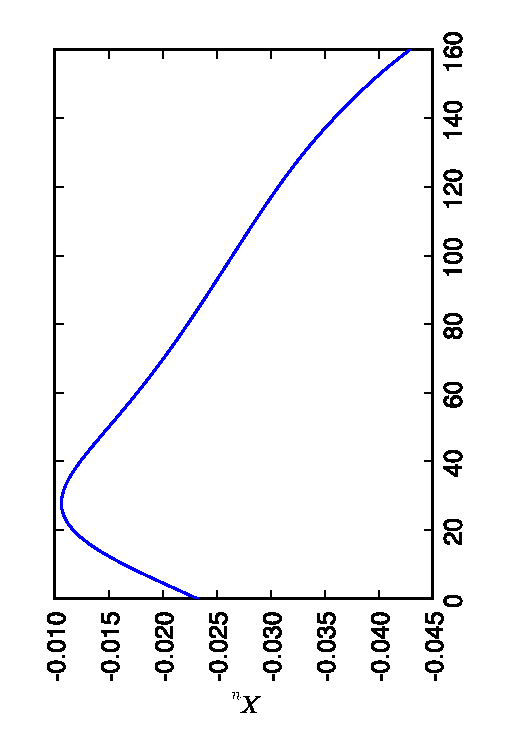
\includegraphics[width=6cm,height=12cm,angle=-90]{Figuras/Lynx_X_u.eps}
	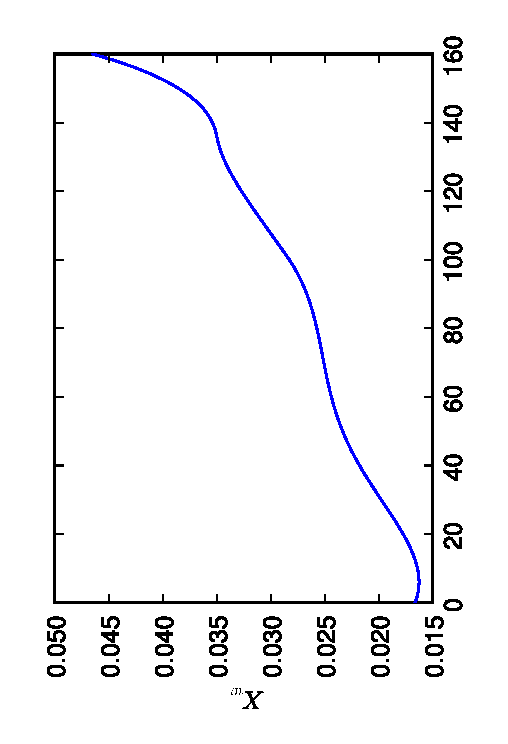
\includegraphics[width=6cm,height=12cm,angle=-90]{Figuras/Lynx_X_w.eps}
	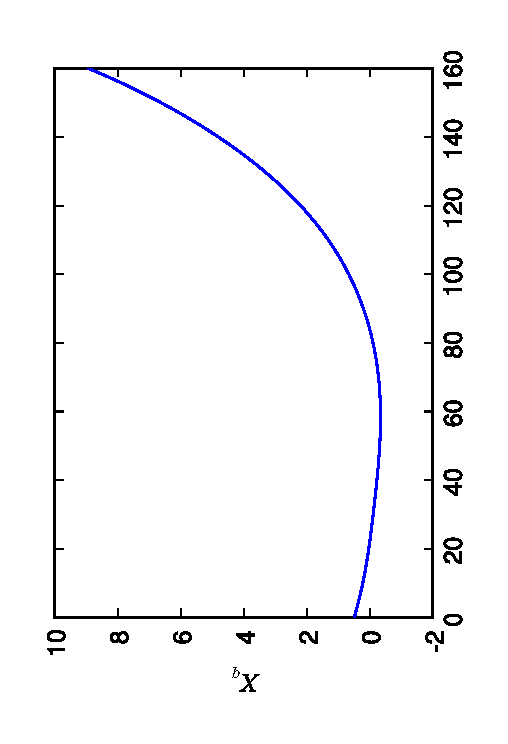
\includegraphics[width=6cm,height=12cm,angle=-90]{Figuras/Lynx_X_q.eps}
\end{figure}

\begin{figure}[h]
	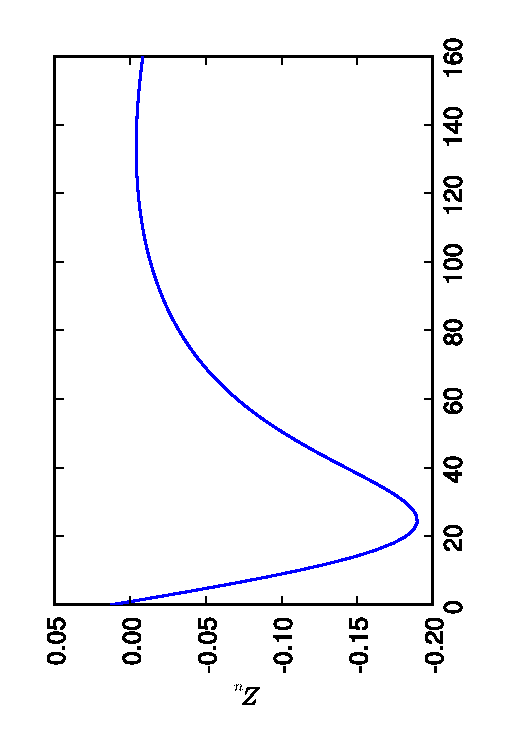
\includegraphics[width=6cm,height=12cm,angle=-90]{Figuras/Lynx_Z_u.eps}
	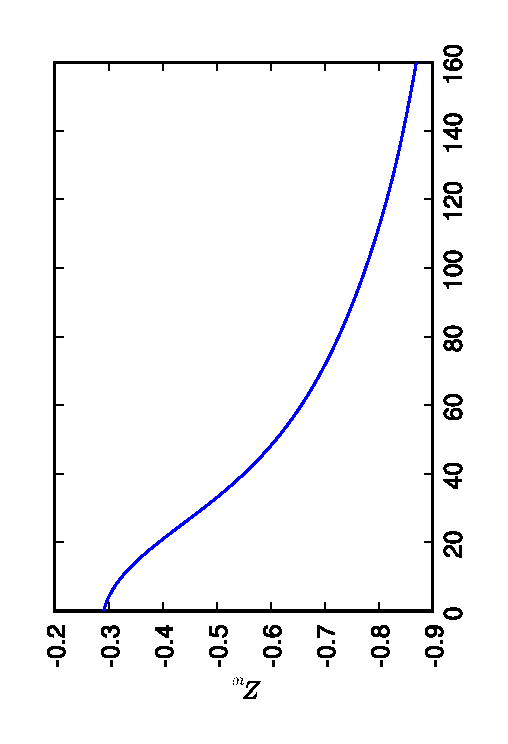
\includegraphics[width=6cm,height=12cm,angle=-90]{Figuras/Lynx_Z_w.eps}
	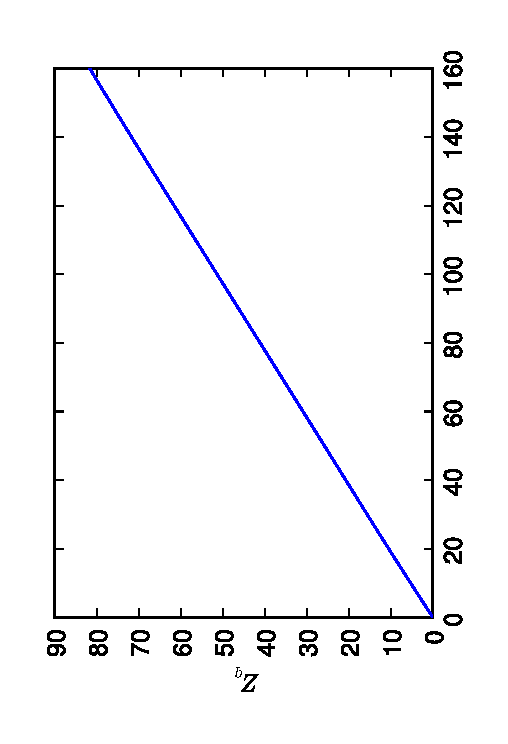
\includegraphics[width=6cm,height=12cm,angle=-90]{Figuras/Lynx_Z_q.eps}
\end{figure}

\begin{figure}[h]
	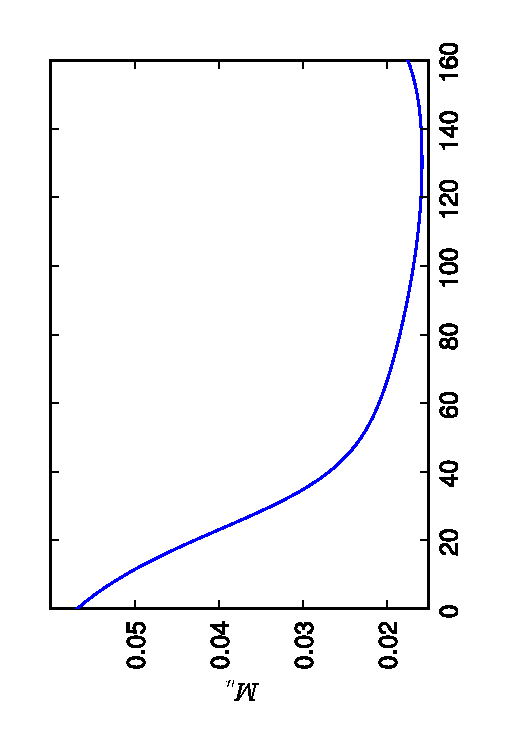
\includegraphics[width=6cm,height=12cm,angle=-90]{Figuras/Lynx_M_u.eps}
	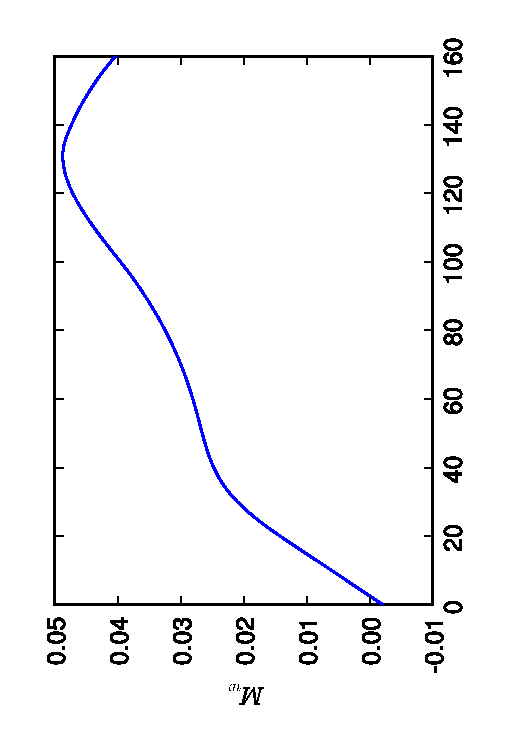
\includegraphics[width=6cm,height=12cm,angle=-90]{Figuras/Lynx_M_w.eps}
	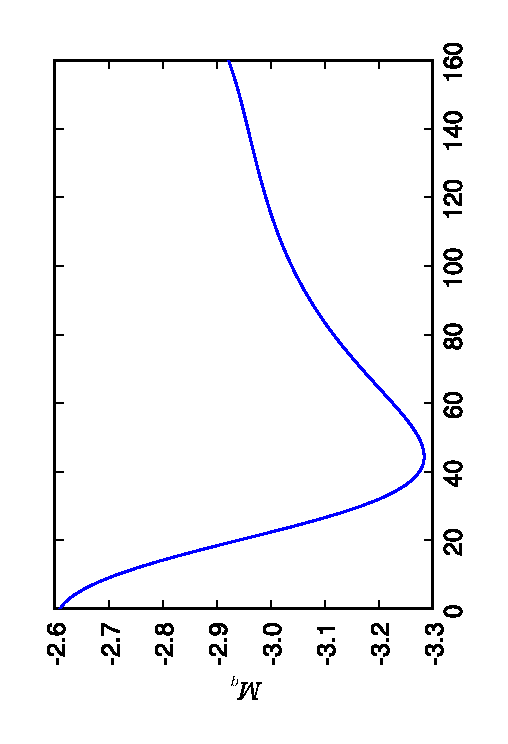
\includegraphics[width=6cm,height=12cm,angle=-90]{Figuras/Lynx_M_q.eps}
\end{figure}

\begin{figure}[h]
	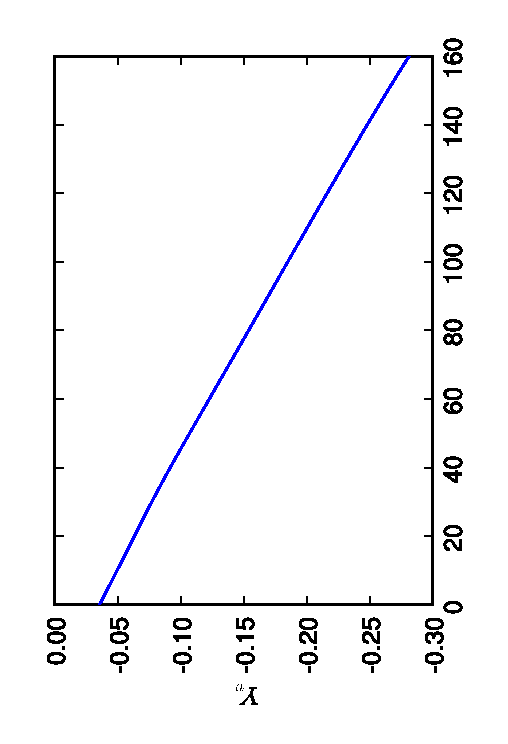
\includegraphics[width=6cm,height=12cm,angle=-90]{Figuras/Lynx_Y_v.eps}
	\includegraphics[width=6cm,height=12cm,angle=-90]{Figuras/Lynx_Y_p.eps}
	\includegraphics[width=6cm,height=12cm,angle=-90]{Figuras/Lynx_Y_r.eps}
\end{figure}

\begin{figure}[h]
	\includegraphics[width=6cm,height=12cm,angle=-90]{Figuras/Lynx_L_v.eps}
	\includegraphics[width=6cm,height=12cm,angle=-90]{Figuras/Lynx_L_p.eps}
	\includegraphics[width=6cm,height=12cm,angle=-90]{Figuras/Lynx_L_r.eps}
\end{figure}

\begin{figure}[h]
	\includegraphics[width=6cm,height=12cm,angle=-90]{Figuras/Lynx_N_v.eps}
	\includegraphics[width=6cm,height=12cm,angle=-90]{Figuras/Lynx_N_p.eps}
	\includegraphics[width=6cm,height=12cm,angle=-90]{Figuras/Lynx_N_r.eps}
\end{figure}
\clearpage
\begin{figure}[h]
	\includegraphics[width=6cm,height=12cm,angle=-90]{Figuras/Lynx_X_v.eps}
	\includegraphics[width=6cm,height=12cm,angle=-90]{Figuras/Lynx_X_p.eps}
	\includegraphics[width=6cm,height=12cm,angle=-90]{Figuras/Lynx_X_r.eps}
\end{figure}

\begin{figure}[h]
	\includegraphics[width=6cm,height=12cm,angle=-90]{Figuras/Lynx_Z_v.eps}
	\includegraphics[width=6cm,height=12cm,angle=-90]{Figuras/Lynx_Z_p.eps}
	\includegraphics[width=6cm,height=12cm,angle=-90]{Figuras/Lynx_Z_r.eps}
\end{figure}

\begin{figure}[h]
	\includegraphics[width=6cm,height=12cm,angle=-90]{Figuras/Lynx_M_v.eps}
	\includegraphics[width=6cm,height=12cm,angle=-90]{Figuras/Lynx_M_p.eps}
	\includegraphics[width=6cm,height=12cm,angle=-90]{Figuras/Lynx_M_r.eps}
\end{figure}

\begin{figure}[h]
	\includegraphics[width=6cm,height=12cm,angle=-90]{Figuras/Lynx_Y_u.eps}
	\includegraphics[width=6cm,height=12cm,angle=-90]{Figuras/Lynx_Y_w.eps}
	\includegraphics[width=6cm,height=12cm,angle=-90]{Figuras/Lynx_Y_q.eps}
\end{figure}

\begin{figure}[h]
	\includegraphics[width=6cm,height=12cm,angle=-90]{Figuras/Lynx_L_u.eps}
	\includegraphics[width=6cm,height=12cm,angle=-90]{Figuras/Lynx_L_w.eps}
	\includegraphics[width=6cm,height=12cm,angle=-90]{Figuras/Lynx_L_q.eps}
\end{figure}

\begin{figure}[h]
	\includegraphics[width=6cm,height=12cm,angle=-90]{Figuras/Lynx_N_u.eps}
	\includegraphics[width=6cm,height=12cm,angle=-90]{Figuras/Lynx_N_w.eps}
	\includegraphics[width=6cm,height=12cm,angle=-90]{Figuras/Lynx_N_q.eps}
\end{figure}
\clearpage
\begin{figure}[h]
	\includegraphics[width=6cm,height=12cm,angle=-90]{Figuras/Lynx_X_th0.eps}
	\includegraphics[width=6cm,height=12cm,angle=-90]{Figuras/Lynx_X_th1s.eps}
	\includegraphics[width=6cm,height=12cm,angle=-90]{Figuras/Lynx_X_th1c.eps}
\end{figure}

\begin{figure}[h]
	\includegraphics[width=6cm,height=12cm,angle=-90]{Figuras/Lynx_Z_th0.eps}
	\includegraphics[width=6cm,height=12cm,angle=-90]{Figuras/Lynx_Z_th1s.eps}
	\includegraphics[width=6cm,height=12cm,angle=-90]{Figuras/Lynx_Z_th1c.eps}
\end{figure}

\begin{figure}[h]
	\includegraphics[width=6cm,height=12cm,angle=-90]{Figuras/Lynx_M_th0.eps}
	\includegraphics[width=6cm,height=12cm,angle=-90]{Figuras/Lynx_M_th1s.eps}
	\includegraphics[width=6cm,height=12cm,angle=-90]{Figuras/Lynx_M_th1c.eps}
\end{figure}

\begin{figure}[h]
	\includegraphics[width=6cm,height=12cm,angle=-90]{Figuras/Lynx_Y_th0.eps}
	\includegraphics[width=6cm,height=12cm,angle=-90]{Figuras/Lynx_Y_th1s.eps}
	\includegraphics[width=6cm,height=12cm,angle=-90]{Figuras/Lynx_Y_th1c.eps}
\end{figure}

\begin{figure}[h]
	\includegraphics[width=6cm,height=12cm,angle=-90]{Figuras/Lynx_L_th0.eps}
	\includegraphics[width=6cm,height=12cm,angle=-90]{Figuras/Lynx_L_th1s.eps}
	\includegraphics[width=6cm,height=12cm,angle=-90]{Figuras/Lynx_L_th1c.eps}
\end{figure}

\begin{figure}[h]
	\includegraphics[width=6cm,height=12cm,angle=-90]{Figuras/Lynx_N_th0.eps}
	\includegraphics[width=6cm,height=12cm,angle=-90]{Figuras/Lynx_N_th1s.eps}
	\includegraphics[width=6cm,height=12cm,angle=-90]{Figuras/Lynx_N_th1c.eps}
\end{figure}

\begin{figure}[h]
	\includegraphics[width=6cm,height=12cm,angle=-90]{Figuras/Lynx_X_th0T.eps}
	\includegraphics[width=6cm,height=12cm,angle=-90]{Figuras/Lynx_Z_th0T.eps}
	\includegraphics[width=6cm,height=12cm,angle=-90]{Figuras/Lynx_M_th0T.eps}
\end{figure}

\begin{figure}[h]
	\includegraphics[width=6cm,height=12cm,angle=-90]{Figuras/Lynx_Y_th0T.eps}
	\includegraphics[width=6cm,height=12cm,angle=-90]{Figuras/Lynx_L_th0T.eps}
	\includegraphics[width=6cm,height=12cm,angle=-90]{Figuras/Lynx_N_th0T.eps}
\end{figure}

\section{C�lculo de la respuesta}
Se incluye un peque�o fichero de ejemplo \verb!ensayos.py! que permite 
calcular la respuesta del helic�ptero y muestra los resultados que se incluyen
a continuaci�n para entradas escal�n a partir de vuelo trimado.

\begin{figure}[h]
	\includegraphics[scale=0.5]{Figuras/ensayo_hor_et1sp.eps}
    \caption{Entrada escal�n para mando longitudinal a partir de vuelo trimado
    horizontal a 30 m/s: piloto}
\end{figure}

\begin{figure}[h]
	\includegraphics[scale=0.5]{Figuras/ensayo_hor_th1s.eps}
    \caption{Entrada escalon para mando longitudinal a partir de vuelo trimado
    horizontal a 30 m/s: paso longitudinal}
\end{figure}

\begin{figure}[h]
	\includegraphics[scale=0.5]{Figuras/ensayo_hor_u.eps}
    \caption{Entrada escalon para mando longitudinal a partir de vuelo trimado
    horizontal a 30 m/s: velocidad horizontal}
\end{figure}

\begin{figure}[h]
	\includegraphics[scale=0.5]{Figuras/ensayo_hor_w.eps}
    \caption{Entrada escalon para mando longitudinal a partir de vuelo trimado
    horizontal a 30 m/s: velocidad vertical}
\end{figure}

\begin{figure}[h]
	\includegraphics[scale=0.5]{Figuras/ensayo_hor_q.eps}
    \caption{Entrada escalon para mando longitudinal a partir de vuelo trimado
    horizontal a 30 m/s: velocidad angular de cabeceo}
\end{figure}

\begin{figure}[h]
	\includegraphics[scale=0.5]{Figuras/ensayo_fijo_et0p.eps}
    \caption{Entrada escalon para colectivo a partir de vuelo a punto fijo: piloto}
\end{figure}

\begin{figure}[h]
	\includegraphics[scale=0.5]{Figuras/ensayo_fijo_w.eps}
    \caption{Entrada escalon para colectivo a partir de vuelo a punto fijo: 
    velocidad vertical}
\end{figure}


% Apendices
\appendix
\chapter{Manual de Usuario}

\section{Requerimientos}
Para el c�lculo de trimado y derivadas de estabilidad se requieren los 
siguientes programas y librer�as:
\begin{itemize}
    \item python 2.4
    \item numarray
\end{itemize}

Para representar en tiempo real el helic�ptero y pilotarlo:
\begin{itemize}
    \item FlightGear 0.9.10
\end{itemize}

\section{Contenidos del CD}
En la distribuci�n se incluyen al menos los siguientes ficheros:
\begin{itemize}
    \item \verb!bin! 
        \begin{itemize} 
            \item \verb!icaro!
            \item \verb!c_colision.so!
            \item \verb!serializa!
            \item \verb!trimado!
            \item \verb!derivadas!
        \end{itemize}
        \verb!icaro! es el programa m�s importante y se incluye una descripci�n a 
        continuaci�n. \verb!serializa!, \verb!trimado! y \verb!derivadas! son 
        utilidades para el c�lculo de diversos resultados, que se han utilizado en la 
        realizaci�n del proyecto y \verb!c_colision.so! es simplemente una librer�a de 
        C que se necesita (su c�digo se encuentra disponible en \verb!src!).
    \item \verb!src!
        Contiene el c�digo fuente necesario para el funcionamiento del simulador
    \item \verb!txt! 
        Contiene el c�digo \LaTeX de la memoria, y todas las figuras en formato
        postscript y en el formato original necesarias.
    \item \verb!dat!
        \begin{itemize}
            \item \verb!runfgfs.sh!: un script con las opciones t�picas para
                invocar a FlightGear.
            \item \verb!X52.xml!: fichero con la descripci�n del joystick
                de la marca Saitek.
            \item \verb!prop-pedals-usb.xml!.: fichero con la descripci�n de los 
                pedales de la marca CH.
            \item \verb!Lynx!: Contiene la descripci�n del helic�ptero Lynx 
                necesaria para el funcionamiento de FlightGear. 
        \end{itemize}
\end{itemize}



\section{icaro}
Para realizar un vuelo el primer paso es ejecutar \verb!icaro!, como m�nimo
especificando el modelo a utilizar. Por ejemplo, si en el directorio actual se
encuentra el fichero \verb!Lynx.py! que contiene una descripci�n completa
del modelo, el arranque del programa tendr�a el siguiente aspecto:

\begin{Verbatim}
$icaro --modelo=Lynx
# INFO: Leyendo modelo de helicoptero Lynx
# INFO: Iniciando conexion de entrada de controles
# INFO: Entrando en el bucle de la simulacion.
# INFO: Presione Ctrl-C para cancelar la simulacion.
\end{Verbatim}

En este punto el simulador se queda esperando una conexi�n a FlightGear, por
lo que arrancar�amos este �ltimo con, por lo menos, las siguientes opciones:

\begin{Verbatim}
$fgfs --fdm=network,localhost,5001,5002,5003 --aircraft=Lynx 
--enable-hud --model-hz=35
\end{Verbatim}

Es importante especificar un valor correcto para la opci�n \verb!--modelo-hz! 
ya que es la frecuencia con que se ejecuta el modelo, por lo que tiene que ser
suficientemente elevada para garantizar la convergencia del integrador y 
suficientemente baja para garantizar que de tiempo a realizar el paso de integraci�n.
Para el esquema Predictor-Corrector 35 es un valor aceptable.

Una descripci�n m�s detallada de las opciones se encuentra en la secci�n
dedicada a FlightGear.

Una vez termine de arrancar FlightGear manda a nuestro programa la informaci�n
de posici�n y orientaci�n iniciales, icaro informa de ello:
\begin{Verbatim}
# INFO: Posicion inicial recibida:
# INFO:         longitud = -2.135844 rad
# INFO:         latitud  = 0.656575 rad
# INFO:         altitud  = 1.290497 m
# INFO:         azimuth  = 4.712389 rad
# INFO:         altura del suelo  = 1.290497 m
\end{Verbatim}

Una vez hayamos terminado de volar, cancelamos la simulaci�n pulsando
Ctrl-C:
\begin{Verbatim}
# Deteniendo la simulacion...
# INFO: Cerrando conexiones...
# INFO: Cerrando archivos...
\end{Verbatim}

A la descripci�n completa de las opciones que acepta icaro se puede acceder
desde la l�nea de comandos:
\begin{Verbatim}
$icaro --help

usage: icaro --modelo=M, [--logfile=F, --logprop=a, [b,c...]] [--host=H], 
[--puertos=p0,p1,p2]

options:
  --version          show program's version number and exit
  -h, --help         show this help message and exit
  --modelo=MODELO    Nombre del archivo que contiene el modelo, sin la
                     extension .py
  --logfile=LOGFILE  Fichero opcional de salida de datos para logging
  --logprop=LOGPROP  Propiedades a escribir en el fichero de logging.
                     Consultar documentacion para ver la lista de
                     posibilidades
  --host=HOST        Direccion de la maquina ejecutando FlightGear, si no se
                     especifica se asume localhost
  --puertos=PUERTOS  Puertos de conexion con FlightGear, respectivamente son
                     de controles, del FDM y de comandos. Por defecto son los
                     puertos 5001, 5002 y 5003 respectivamente
\end{Verbatim}

\subsection{Logging}
Es posible almacenar en un fichero la historia temporal de ciertas variables;
esto permite consultar m�s tarde los resultados en el fichero o incluso
mostrarlos en pantalla en tiempo real.

Las variables que se quieran ir guardando se especifican en la l�nea de 
comandos como una lista separada por comas. Por ejemplo:

\begin{Verbatim}
$icaro --modelo=Lynx --logfile=vuelo.dat --logprop=u,v,w
\end{Verbatim}

El simulador en este caso crear�a el fichero \verb!vuelo.dat! si no existe, y si
existe, sobreescribir�a encima y guardar�a para cada instante de tiempo que
calcule 4 columnas de datos. La primera columna indica el instante de tiempo y
las restantes columnas las variables que se han especificado mediante
\verb!--logprop=u,v,w!, en este caso la velocidad en ejes cuerpo, en el mismo
orden en que se han especificado.

En caso de que se pida una variable que no se encuentre calculada, bien porque
se haya cometido un error tipogr�fico o porque no se pueda realizar
el c�lculo, el programa le asigna un valor de 0 y contin�a.

Si se quiere visualizar interactivamente los resultados durante la simulaci�n,
el fichero de salida tiene ese formato precisamente para poder utilizarlo
directamente con el programa \verb!kst! (\url{http://kst.kde.org}). Para ello, 
mientras corre la simulaci�n, deber�amos haber ejecutado:
\begin{Verbatim}
$kst -x1 -y2 -y3 -y4 -m1 vuelo.dat
\end{Verbatim}

Si se quiere manipular la salida se puede pasar el fichero de logging a 
c�digo en python. Se
incluye una peque�a utilidad \verb!serializa! que crea un interpolador
lineal en funci�n del tiempo para cada columna del fichero. Por ejemplo,
para utilizar en una sesi�n de python el fichero \verb!vuelo.dat! del 
ejemplo anterior ejecutar�amos:
\begin{Verbatim}
$serializa -i vuelo.dat -o vuelo.pickle
\end{Verbatim}

A continuaci�n cargar�amos las variables en las sesi�n de python:
\begin{Verbatim}
    import pickle
    f = open('vuelo.pickle', 'r')
    u = pickle.load(f)
    v = pickle.load(f)
    w = pickle.load(f)
\end{Verbatim}

Ahora ya podemos manipular tranquilamente \verb!u!, \verb!v! y \verb!w! con
nuestro c�digo. Por ejemplo, mostr�ndolo por pantalla:
\begin{Verbatim}
    import pylab
    pylab.plot(u.x, u.y)
    pylab.plot(v.x, v.y)
    pylab.plot(w.x, w.y)
    pylab.show()
\end{Verbatim}

Los objetos creados son interpoladores lineales tal como se encuentran
definidos en \verb!matematicas.py!. Disponen de dos atributos que contienen 
las coordenadas de los puntos que interpolan: \verb!x! e \verb!y! y pueden
ser llamados como funci�n para que calculen al valor en un punto arbitrario.

A continuaci�n se da la lista de variables que se pueden pasar como argumentos,
a \verb!--logprop!, una descripci�n de su significado y el s�mbolo matem�tico 
asociado.

\subsubsection{General}
\begin{itemize}
    \item \verb!u! ($u$), \verb!v! ($v$), \verb!w! ($w$): componentes de la 
        velocidad del helic�ptero en ejes cuerpo, en metros por segundo.
    \item \verb!p! ($p$), \verb!q! ($q$), \verb!r! ($r$): componentes de la 
        velocidad angular del helic�ptero en ejes cuerpo, 
        en radianes por segundo.
    \item \verb!q0! ($q_0$), \verb!q1! ($q_1$), \verb!q2! ($q_2$), 
        \verb!q3! ($q_3$): componentes del cuaternio de rotaci�n.

    \item \verb!th! ($\theta$): �ngulo de cabeceo, en radianes.
    \item \verb!fi! ($\phi$): �ngulo de balance, en radianes.
    \item \verb!ch! ($\psi$): �ngulo de gui�ada, en radianes.
    
    \item \verb!alt! ($h$): altitud, en metros.
    \item \verb!lon! ($\lambda$): longitud, en radianes.
    \item \verb!lat! ($\phi$): latitud, en radianes.
    
    \item \verb!x_i! ($x_i$), \verb!y_i! ($y_i$), \verb!z_i! ($z_i$): posici�n 
        en ejes inerciales 
\end{itemize}

\subsubsection{Rotor principal}
\begin{itemize}
    \item \verb!la0! ($\lambda_0$), \verb!la1cw! ($\lambda_{1cw}$), 
        \verb!la1sw! ($\lambda_{1sw}$): componentes de la velocidad inducida, 
        en ejes rotor-viento.
    \item \verb!be0! ($\beta_0$), \verb!be1cw! ($\beta_{1cw}$),  
        \verb!be1sw! ($\beta_{1sw}$): componentes del batimiento, en ejes
        rotor-viento.
    \item \verb!cT! ($c_T$): coeficiente de sustentaci�n del rotor.
    \item \verb!XR_b! ($X_{R_b}$), \verb!YR_b! ($Y_{R_b}$), 
        \verb!ZR_b! ($Z_{R_b}$): componentes de las fuerzas del rotor sobre el 
        centro de masas en ejes cuerpo, en Newtons.
    \item \verb!LR_b! ($L_{R_b}$), \verb!MR_b! ($M_{R_b}$), 
        \verb!NR_b! ($N_{R_b}$): componentes de los momentos del rotor sobre 
        el centro de masas en ejes cuerpo, en Newtons por metro.
\end{itemize}
    
\subsubsection{Fuselaje}
\begin{itemize}
    \item \verb!alf! ($\alpha_f$): �ngulo de ataque del fuselaje, en radianes.
    \item \verb!bef! ($\beta_f$): �ngulo de resbalamiento del fuselaje, en 
        radianes.
    \item \verb!Xf_b! ($X_{f_b}$), \verb!Yf_b! ($Y_{f_b}$), 
        \verb!Zf_b! ($Z_{f_b}$): componentes de las fuerzas del fuselaje sobre 
        el centro de masas en ejes cuerpo.
    \item \verb!Lf_b! ($L_{f_b}$), \verb!Mf_b! ($M_{f_b}$), 
        \verb!Nf_b! ($N_{f_b}$): componentes de los momentos del fuselaje sobre
        el centro de masas en ejes cuerpo.
\end{itemize}

\subsubsection{Controles}
\begin{itemize}
    \item \verb!th0! ($\theta_0$), \verb!th1c! ($\theta_{1c}$),
        \verb!th1s! ($\theta_{1s}$): componentes del paso del rotor en ejes 
        rotor, en radianes.
    \item \verb!th0T! ($\theta_{0_T}$): paso del rotor de cola en radianes.
    \item \verb!eta0p! ($\eta_{0p}$): control colectivo del piloto. 
        Normalizado de 0 a 1.
    \item \verb!eta1sp! ($\eta_{1s}$): control longitudinal del piloto. 
        Normalizado de -1 a +1.
    \item \verb!eta1cp! ($\eta_{1c}$): control lateral del piloto. 
        Normalizado de -1 a +1.
    \item \verb!etapp! ($\eta_{pp}$): control de pedales del piloto. 
        Normalizado de -1 a +1.
\end{itemize}

\subsubsection{Motor}
\begin{itemize}
    \item \verb!Om! ($\Omega$): velocidad de giro del rotor en rad/s.
    \item \verb!Q1! ($Q_1$): par de un motor.
    \item \verb!DTQ1! ($\dot{Q}_1$): derivada del par de un motor.
\end{itemize}
    
\subsubsection{Rotor de cola}
\begin{itemize}
    \item \verb!cTT! ($c_{T_T}$): coeficiente de sustentaci�n del rotor de cola.
    \item \verb!la0T! ($la0T$): velocidad inducida en el rotor de cola.
    \item \verb!XT_b! ($X_{T_b}$), \verb!YT_b! ($Y_{T_b}$),
        \verb!ZT_b! ($Z_{T_b}$): componentes de las fuerzas del rotor de cola 
        sobre el centro de masas, en ejes cuerpo.
    \item \verb!LT_b! ($L_{T_b}$), \verb!MT_b! ($M_{T_b}$), 
        \verb!NT_b! ($N_{T_b}$): componentes de los momentos del rotor de cola
        sobre el centro de masas, en ejes cuerpo.
\end{itemize}
    
\subsubsection{Estabilizador vertical}
\begin{itemize}
    \item \verb!alfn! ($\alpha_{fn}$): �ngulo de ataque del estabilizador 
        vertical, en radianes.
    \item \verb!befn! ($\beta_{fn}$): �ngulo de resbalamiento del 
        estabilizador vertical, en radianes.
    \item \verb!Xfn_b! ($X_{fn_b}$), \verb!Yfn_b! ($Y_{fn_b}$), 
        \verb!Zfn_b! ($Z_{fn_b}$): componentes de las fuerzas del 
        estabilizador vertical sobre el centro de masas, en ejes cuerpo.
    \item \verb!Lfn_b! ($L_{fn_b}$), \verb!Mfn_b! ($M_{fn_b}$), 
        \verb!Nfn_b! ($N_{fn_b}$): componentes de los momentos del 
        estabilizador vertical sobre el centro de masas, en ejes cuerpo.
\end{itemize}
    
\subsubsection{Estabilizador horizontal}
\begin{itemize}
    \item \verb!altp! ($\alpha_{tp}$): �ngulo de ataque del estabilizador 
        horizontal, en radianes.
    \item \verb!betp! ($\beta_{tp}$): �ngulo de resbalamiento del 
        estabilizador  horizontal, en radianes.
    \item \verb!Xtp_b! ($X_{tp_b}$), \verb!Ytp_b! ($Y_{tp_b}$), 
        \verb!Ztp_b! ($Z_{tp_b}$): componentes de las fuerzas del 
        estabilizador horizontal sobre el centro de masas, en ejes cuerpo.
    \item \verb!Lfn_b! ($L_{tp_b}$), \verb!Mtp_b! ($M_{tp_b}$), 
        \verb!Nfn_b! ($N_{tp_b}$): componentes de los momentos del 
        estabilizador horizontal sobre el centro de masas, en ejes cuerpo.
\end{itemize}

\section{FlightGear}

\subsection{Introducci�n}

FlightGear (en adelante referido como FGFS, FlightGear Flight Simulator), es un 
simulador de vuelo distribuido bajo licencia GPL (GNU General Public License) 
totalmente gratis. La p�gina oficial del proyecto se encuentra
en \url{http://www.flightgear.org} y se puede leer una buena introducci�n a la
estructura del proyecto en \cite{fgfs}. FGFS presenta las siguientes caracter�sticas
interesantes para el desarrollo de este proyecto fin de carrera:

\begin{itemize}
    \item Al ser licencia GPL se tiene acceso al c�digo fuente, para leerlo y
    para modificarlo. Hubiese sido posible por ejemplo integrar el c�digo
    del simulador de helic�pteros en C++ dentro del propio programa
    FlightGear (cosa que no se ha hecho como se explica m�s adelante). S� se
    ha utilizado dicha libertad de acceso al c�digo fuente para estudiar el
    protocolo de transmisi�n entre FlightGear y programas externos a traves
    de sockets.

    \item Ha sido dise�ado pensando en la adaptaci�n a las necesidades de cada
    usuario. Resulta interesante, en particular, para proyectos de car�cter
    acad�mico y otros que se salgan de los intereses de la mayor�a del
    mercado. Para ver una lista de proyectos que utilizan FGFS consultar
    \url{http://www.flightgear.org/Projects/}

    \item Est� pensado para interaccionar con �l mediante otros programas.
    Todo el estado del simulador, desde el modelo 3D del helic�ptero, su
    posici�n, etc.. hasta la indicaci�n de cualquier instrumento y el estado
    meteorol�gico se encuentra organizado en forma de �rbol, simulando un
    sistema de archivos, al que se puede acceder desde diversos medios:
    telnet, http desde cualquier navegador web, sockets y tuber�as.

    \item Formatos abiertos: los ficheros de configuraci�n se encuentran en
    XML, esto permite trabajar con ellos desde cualquier editor de
    textos, adem�s resultan bastante claros y sencillos. Hay una
    gran cantidad de aeronaves ya preparadas para, a partir de las cuales,
    crear tu propio fichero de configuraci�n.

    \item Multiplataforma: Funciona tanto en Linux como en Windows o Mac. De
    hecho, es posible tener un ordenador con Linux ejecutando el FDM y otro
    con Windows encargandose de la entrada/salida con el usuario.

    \item Modularidad: En FGFS se encuentran separados claramente las partes
    encargadas de la entrada/salida de datos del FDM. De hecho, FGFS viene
    con 3 FDM ya incluidos: UUIC, YaSim y JSBSim. Esta separaci�n permite
    que le podamos a�adir un cuarto FDM especializado para helic�pteros, que
    es el objeto de este proyecto fin de carrera.
\end{itemize}

\subsection[Integraci�n FG-FDM]{Integraci�n de FlightGear con el FDM de helic�pteros}
El simulador consta, por lo tanto de varios programas, operando simult�neos en uno
o varios ordenadores y que se comunican entre ellos utilizando diversos
protocolos, como se puede ver en la figura.

\begin{figure}
    \includegraphics[scale=0.5]{Figuras/esquema_flightgear.eps}
\end{figure}

FGFS y el FDM se comunican a traves de 3 canales como se puede ver en la figura:
controles, estado y comandos. Cada uno de ellos requiere de un puerto distinto
por lo que al iniciar FGFS es necesario indicar en la l�nea de comandos que el
FDM va a ser un programa aparte, el ordenador donde se encuentra y los puertos
de comunicaci�n. Por ejemplo:

\begin{Verbatim}
$fgfs --fdm=network,localhost,5001,5002,5003
\end{Verbatim}

arranca FGFS y especifica que el FDM correr� en el mismo ordenador que FGFS y
utilizar� el puerto 5001 para los controles, el puerto 5002 para el estado del
FDM y el 5003 para los comandos.

Generalmente es necesario pasar m�s opciones, por ejemplo:

\begin{Verbatim}
$fgfs --aircraft=Lynx --airport=LEVS  --httpd=5080 
--fdm=network,localhost,5001,5002,5003
\end{Verbatim}

Arrancar�a FGFS utilizando el helic�ptero Lynx, situandolo inicialmente en
el aeropuerto de Cuatro Vientos. Adem�s especifica como antes los puertos de
comunicaci�n con el FDM y a�ade un canal de comunicaci�n en el puerto 5080 para
poder inspeccionar y modificar el estado del simulador en tiempo real mediante
un navegador web. En la imagen se puede observar como es posible acceder por
ejemplo a todas las variables meteorol�gicas y modificarlas mediante el
navegador web. Recordemos que no es necesario acceder desde el mismo ordenador.
En el anterior caso un instructor podr�a estar modificando las variables
atmosf�ricas desde cualquier otro ordenador, sea en una LAN o incluso Internet.

\begin{figure}
    \includegraphics[scale=0.35]{Figuras/HTTP.eps}
\end{figure}

\subsection[Comunicaci�n]{Canales de comunicaci�n con el FDM}
No existe documentaci�n del protocolo de transmisi�n, aparte del c�digo fuente
de FGFS. B�sicamente FGFS crea una estructura, la rellena con los datos a
transmitir y la manda tal cual a trav�s de un socket UDP. El FDM debe crear una
estructura espejo a la anterior y copiar tal cual en memoria los datos
recibidos. La estructura de los controles que FGFS manda al FDM y la estructura
de estado que el FDM manda a FGFS se encuentra definida en 

\begin{Verbatim}
    $FGSRC/src/Network/net_ctrls.hxx
    $FGSRC/src/Network/net_fdm.hxx
\end{Verbatim}

Donde \verb#$FGSRC# indica el directorio ra�z del c�digo fuente de FGFS

El canal de comandos utiliza protocolo HTTP y manda informaci�n al inicio de la
simulaci�n al FDM con la posici�n inicial de la aeronave.
Se encuentra definido en

\begin{Verbatim}
    $FGSRC/src/FDM/ExternalNet/ExternalNet.hxx 
    $FGSRC/src/FDM/ExternalNet/ExternalNet.cxx 
\end{Verbatim}

\subsection{Ficheros de FlightGear}
Es necesario indicar a FGFS la aeronave a utilizar. Se puede obtener una lista
de las aeronaves disponibles con la opci�n -\verb#--show-aircraft# que
determinar� las aeronaves disponibles en funci�n de lo que encuentre en el
directorio

\begin{Verbatim}
    $FGROOT/Aircraft
\end{Verbatim}

Donde cada nave tiene su propio subdirectorio. Se ha incluido ya un archivo
listo para descomprimir en el directorio de aeronaves que contiene la
descripci�n necesaria para FGFS del Lynx. Dicho archivo contiene el modelo
3D, las texturas del modelo y los dos archivos XML con la configuraci�n y
descripci�n del panel de instrumentos.

Tambi�n es necesario disponer de los terrenos necesarios. Para ello es necesario
bajarse e instalar manualmente los archivos en el directorio

\begin{Verbatim}
    $FGROOT/Scenery
\end{Verbatim}

o utilizar la utilidad TerraSync, un programa aparte que se baja los archivos
seg�n sean necesarios desde internet. Se han incluido ya los dos archivos
necesarios para la pen�nsula ib�rica listos para descomprimir en el directorio
de escenarios.

Para m�s informaci�n consultar la documentaci�n de FlightGear. 

\chapter{C�digo}
\definecolor{MidGray}{rgb}{0.5,0.5,0.5}
\lstset{
        language=python,
        extendedchars=true,
        showspaces=false,
        showstringspaces=false,
        basicstyle=\footnotesize\ttfamily\color{Black},
        stringstyle=\itshape\color{Blue},
        commentstyle=\color{MidGray},
        breaklines=false,
        columns=fixed,
        linewidth=42em,
        keywordstyle=\bfseries\color{Red},
        }

\section{icaro.py}
\lstinputlisting[frame=single]{/home/asmodeus/PFC/src/icaro.py}

\section{flightgear.py}
\lstinputlisting[frame=single]{/home/asmodeus/PFC/src/flightgear.py}

\section{modelo.py}
\lstinputlisting[frame=single]{/home/asmodeus/PFC/src/modelo.py}

\section{rotor.py}
\lstinputlisting[frame=single]{/home/asmodeus/PFC/src/rotor.py}

\section{rotor\textunderscore cola.py}
\lstinputlisting[frame=single]{/home/asmodeus/PFC/src/rotor_cola.py}

\section{fuselaje.py}
\lstinputlisting[frame=single]{/home/asmodeus/PFC/src/fuselaje.py}

\section{estabilizador.py}
\lstinputlisting[frame=single]{/home/asmodeus/PFC/src/estabilizador.py}

\section{controles.py}
\lstinputlisting[frame=single]{/home/asmodeus/PFC/src/controles.py}

\section{motor.py}
\lstinputlisting[frame=single]{/home/asmodeus/PFC/src/motor.py}

\section{colision.py}
\lstinputlisting[frame=single]{/home/asmodeus/PFC/src/colision.py}

\section{algebra.h}
\lstinputlisting[frame=single,language=C]{/home/asmodeus/PFC/src/algebra.h}

\section{algebra.c}
\lstinputlisting[frame=single,language=C]{/home/asmodeus/PFC/src/algebra.c}

\section{colision.h}
\lstinputlisting[frame=single,language=C]{/home/asmodeus/PFC/src/colision.h}

\section{colision.c}
\lstinputlisting[frame=single,language=C]{/home/asmodeus/PFC/src/colision.c}

\section{integrador.py}
\lstinputlisting[frame=single]{/home/asmodeus/PFC/src/integrador.py}

\section{historial.py}
\lstinputlisting[frame=single]{/home/asmodeus/PFC/src/historial.py}

\section{aero.py}
\lstinputlisting[frame=single]{/home/asmodeus/PFC/src/aero.py}

\section{input.py}
\lstinputlisting[frame=single]{/home/asmodeus/PFC/src/input.py}

\section{protocolo.py}
\lstinputlisting[frame=single]{/home/asmodeus/PFC/src/protocolo.py}

\section{matematicas.py}
\lstinputlisting[frame=single]{/home/asmodeus/PFC/src/matematicas.py}

\section{geodesia.py}
\lstinputlisting[frame=single]{/home/asmodeus/PFC/src/geodesia.py}

\section{Lynx.py}
\lstinputlisting[frame=single]{/home/asmodeus/PFC/src/Lynx.py}

%\section{UH60.py}
%\lstinputlisting[frame=single]{/home/asmodeus/PFC/src/UH60.py}

\section{derivadas.py}
\lstinputlisting[frame=single]{/home/asmodeus/PFC/src/derivadas.py}


%%%%%%%%%%%%%%%%%%%%%%%%%%%%%%%%%%%%%%%%%%%%%%%%%%%%%%%%%%%%%%%%%%%%%%%%%%%%%%%%
% Final                                                                        %
%%%%%%%%%%%%%%%%%%%%%%%%%%%%%%%%%%%%%%%%%%%%%%%%%%%%%%%%%%%%%%%%%%%%%%%%%%%%%%%%
\backmatter
\bibliographystyle{plain}
\bibliography{memoria}
\end{document}
